\documentclass[11pt,a4paper]{article}
\usepackage[T1]{fontenc}\usepackage{lmodern}
\usepackage[a4paper,margin=23mm,includeheadfoot,headheight=15pt,headsep=15pt,footskip=22pt]{geometry}
\usepackage[nopatch=footnote]{microtype}
\usepackage{amsmath,amssymb,amsthm,mathtools,amscd,aliascnt}
\usepackage{booktabs,longtable,array,tabularx,enumitem,fancyhdr,graphicx}
\usepackage[table]{xcolor}\usepackage{setspace,needspace,listings,caption,titlesec,etoolbox,bm,float}
\usepackage{xurl}\usepackage{hyperref}\usepackage[nameinlink,noabbrev]{cleveref}\usepackage{bookmark}
\definecolor{accent}{HTML}{137668}\definecolor{muted}{HTML}{536568}
\definecolor{leanblue}{RGB}{20,72,135}\definecolor{roadmapgray}{RGB}{86,86,86}
\frenchspacing\emergencystretch=3em\clubpenalty=10000\widowpenalty=10000\raggedbottom
\titleformat{\section}{\sffamily\bfseries\large\color{accent}}{\thesection}{.7em}{}
\titleformat{\subsection}{\sffamily\bfseries\normalsize}{\thesubsection}{.7em}{}
\titlespacing*{\section}{0pt}{1.4\baselineskip}{.55\baselineskip}
\captionsetup{font=small,labelfont={sf,bf},labelsep=period}
\pretocmd{\section}{\Needspace{7\baselineskip}}{}{}\pretocmd{\subsection}{\Needspace{5\baselineskip}}{}{}
\allowdisplaybreaks\setstretch{1.055}\setlength{\parskip}{.3em}\setlength{\parindent}{1.35em}
\setlist[itemize]{topsep=.35em,itemsep=.15em,leftmargin=1.6em}\setlist[enumerate]{topsep=.35em,itemsep=.15em,leftmargin=1.8em}
\graphicspath{{figures/}}
\hypersetup{pdftitle={Projector-Resolved Seed Calculus III: Typed Transfer, Nonlinear Packets and Obstruction Theory},pdfauthor={Komorebi P.},colorlinks=true,linkcolor=accent,citecolor=accent,urlcolor=accent}
\pagestyle{fancy}\fancyhf{}
\fancyhead[L]{\sffamily\fontsize{8}{10}\selectfont\color{muted}KOMOREBI MATHEMATICS / PAPER III}
\fancyhead[R]{\sffamily\fontsize{8}{10}\selectfont\color{muted}TRADITIONAL PAPER}
\fancyfoot[L]{\sffamily\fontsize{8}{10}\selectfont\color{muted}Projector-resolved seed calculus}\fancyfoot[R]{\sffamily\small\color{accent}\thepage}
\lstset{basicstyle=\ttfamily\footnotesize,breaklines=true,frame=single,showstringspaces=false,columns=fullflexible,keepspaces=true}
\newtheorem{theorem}{Theorem}[section]
\theoremstyle{plain}
\newaliascnt{proposition}{theorem}
\newtheorem{proposition}[proposition]{Proposition}
\aliascntresetthe{proposition}
\crefname{proposition}{proposition}{propositions}
\newaliascnt{lemma}{theorem}
\newtheorem{lemma}[lemma]{Lemma}
\aliascntresetthe{lemma}
\crefname{lemma}{lemma}{lemmas}
\newaliascnt{corollary}{theorem}
\newtheorem{corollary}[corollary]{Corollary}
\aliascntresetthe{corollary}
\crefname{corollary}{corollary}{corollarys}
\theoremstyle{definition}
\newaliascnt{definition}{theorem}
\newtheorem{definition}[definition]{Definition}
\aliascntresetthe{definition}
\crefname{definition}{definition}{definitions}
\newaliascnt{example}{theorem}
\newtheorem{example}[example]{Example}
\aliascntresetthe{example}
\crefname{example}{example}{examples}
\newaliascnt{construction}{theorem}
\newtheorem{construction}[construction]{Construction}
\aliascntresetthe{construction}
\crefname{construction}{construction}{constructions}
\newaliascnt{standardfact}{theorem}
\newtheorem{standardfact}[standardfact]{Standard Fact}
\aliascntresetthe{standardfact}
\crefname{standardfact}{standard fact}{standard facts}
\theoremstyle{remark}
\newaliascnt{remark}{theorem}
\newtheorem{remark}[remark]{Remark}
\aliascntresetthe{remark}
\crefname{remark}{remark}{remarks}
\newaliascnt{boundary}{theorem}
\newtheorem{boundary}[boundary]{Boundary}
\aliascntresetthe{boundary}
\crefname{boundary}{boundary}{boundarys}
\newaliascnt{roadmap}{theorem}
\newtheorem{roadmap}[roadmap]{Formalization target}
\aliascntresetthe{roadmap}
\crefname{roadmap}{formalization target}{formalization targets}
\crefname{theorem}{theorem}{theorems}
\newcommand{\bbk}{\Bbbk}
\newcommand{\N}{\mathbb N}
\newcommand{\cA}{\mathcal A}
\newcommand{\cC}{\mathcal C}
\newcommand{\cE}{\mathcal E}
\newcommand{\cG}{\mathcal G}
\newcommand{\cH}{\mathcal H}
\newcommand{\cO}{\mathcal O}
\newcommand{\cP}{\mathcal P}
\newcommand{\cQ}{\mathcal Q}
\newcommand{\cS}{\mathcal S}
\newcommand{\cT}{\mathcal T}
\newcommand{\cW}{\mathcal W}
\newcommand{\End}{\operatorname{End}}
\newcommand{\Hom}{\operatorname{Hom}}
\newcommand{\im}{\operatorname{im}}
\newcommand{\id}{\mathrm{id}}
\newcommand{\Ob}{\operatorname{Ob}}
\newcommand{\Hol}{\operatorname{Hol}}
\newcommand{\Coord}{\operatorname{Coord}}
\newcommand{\ev}{\operatorname{ev}}
\newcommand{\src}{\operatorname{src}}
\newcommand{\tgt}{\operatorname{tgt}}
\newcommand{\Walk}{\operatorname{Walk}}
\newcommand{\supp}{\operatorname{supp}}
\newcommand{\op}{\mathrm{op}}
\newcommand{\leanname}[1]{\nolinkurl{#1}}
\newcommand{\Acal}{\mathcal A}
\newcommand{\Ccal}{\mathcal C}
\newcommand{\Fcal}{\mathcal F}
\newcommand{\Hcal}{\mathcal H}
\newcommand{\Kcal}{\mathcal K}
\newcommand{\Lcal}{\mathcal L}
\newcommand{\Ocal}{\mathcal O}
\newcommand{\Pcal}{\mathcal P}
\newcommand{\Qcal}{\mathcal Q}
\newcommand{\Rcal}{\mathcal R}
\newcommand{\Scal}{\mathcal S}
\newcommand{\Tcal}{\mathcal T}
\newcommand{\Ucal}{\mathcal U}
\newcommand{\Vcal}{\mathcal V}
\newcommand{\Ker}{\operatorname{Ker}}
\newcommand{\coker}{\operatorname{coker}}
\newcommand{\Cone}{\operatorname{Cone}}
\newcommand{\Lip}{\operatorname{Lip}}
\newcommand{\dist}{\operatorname{dist}}
\newcommand{\rank}{\operatorname{rank}}
\newcommand{\MC}{\operatorname{MC}}
\newcommand{\gr}{\operatorname{gr}}
\newcommand{\Span}{\operatorname{span}}
\newcommand{\tr}{\operatorname{tr}}
\newcommand{\Ad}{\operatorname{Ad}}

\newcolumntype{L}[1]{>{\raggedright\arraybackslash}p{#1}}
\newcolumntype{Y}{>{\raggedright\arraybackslash}X}
\newcommand{\statusleanthree}[1]{\par\smallskip\noindent\begin{minipage}{\linewidth}{\color{leanblue}\textbf{Formal contract: Paper III v1.0.1.}}\par\begingroup\small\raggedright\leanname{#1}\par\endgroup\end{minipage}\par\smallskip}
\newcommand{\statusleanprior}[1]{\par\smallskip\noindent\begin{minipage}{\linewidth}{\color{leanblue}\textbf{Inherited formal contract: Papers I--II.}}\par\begingroup\small\raggedright\leanname{#1}\par\endgroup\end{minipage}\par\smallskip}
\newcommand{\statusroadmap}[1]{\par\smallskip\noindent{\color{roadmapgray}\textbf{Outside the finite formal contract.}}\ #1\par\smallskip}

% Operation Komorebi: shared publication profile.
\usepackage{komorebi-publication}
\renewcommand{\KomorebiTitle}{Projector-Resolved Seed Calculus III}
\renewcommand{\KomorebiSubtitle}{Typed transfer, nonlinear packets, and obstruction theory}
\renewcommand{\KomorebiSeries}{Core series III}
\renewcommand{\KomorebiKind}{Traditional paper}
\renewcommand{\KomorebiEdition}{Standardized publication edition / 8 October 2026}
\renewcommand{\KomorebiShortTitle}{Paper III}
\renewcommand{\KomorebiTitleSize}{31}
\renewcommand{\KomorebiTitleLeading}{36}
\renewcommand{\KomorebiProfile}{classical}
\renewcommand{\KomorebiOrientation}{portrait}
\KomorebiSetup
\begin{document}
\KomorebiCover
\KomorebiOpeningNote{\textbf{Reading route.} Typed edge words and exact coordinate transport lead to connection defects and packet obstruction witnesses. Nonlinear packet jets then lead to tree expansions, correction complexes, filtered lifting, elimination, and smooth transport.

\medskip
\textbf{Scope.} Part~I retains the finite v1.0.1 formal contract. Part~II gives the strengthened nonlinear and analytic development with ordinary proofs. Formal coverage stays attached to the exact released declarations and does not extend merely because both parts appear in one edition.}


\begin{abstract}
Finite projector packets turn linear transfer into typed walks and arbitrary maps into exact coordinate representations. We separate canonical coordinate transport, which satisfies an exact cocycle law, from a chosen connection, whose failure to compose produces holonomy and packet obstruction witnesses. We then develop nonlinear packet jets and higher composition, convergent rooted tree expansions, graded operations, and nonlinear refinement defects. A specified correction map produces a canonical cokernel obstruction. Relative exact sequences, mapping cones, Hilbert splitting, nonlinear correction, and filtered lifting describe how these obstructions behave. Exact elimination produces Schur formulas, and finite transport reduces gluing to fundamental cycle holonomy. For smooth orthogonal packet families, direct packet rotations converge in operator norm to canonical unitary transport. The finite formal contract and the broader ordinary proof development are identified separately throughout.
\end{abstract}
\noindent This edition preserves both the finite release and the strengthened nonlinear manuscript. Its companions are a worked visual guide and a Lean guide. The released Lean evidence is inherited; this editorial build does not assert a new Lean execution.
\tableofcontents\listoffigures\clearpage
\part{Finite typed transfer and the formal contract}\label{part:finite}
\noindent The finite release supplies the algebraic foundation and its declaration-level contract. In this part, ``roadmap'' and ``outside the contract'' refer to the finite Lean formalization, not to the absence of ordinary mathematical results in Part~II. The original thirty theorem-like statements and their proof bodies are retained. The source contract has 41 mapping rows, which include definitions and other interfaces and therefore are not the same count as theorem-like statements.

\medskip\noindent The preserved v1.0.1 release records Lean v4.34.0-rc2 against Mathlib revision \leanname{aeb72f1e9981b6d35b426b16dca7759be3e7ba06} \cite{lean,mathlib}. The compiler and kernel-check descriptions in Part~I describe that inherited evidence. Current editorial checks of this edition are recorded separately in the companion verification files.
\section{Purpose and status discipline}
\label{sec:purpose}

Paper I fixed typed seeds, operator grammars, exact projector packets,
generated hulls, and reconstruction \cite{paperI}.  Paper II added coherent
refinement coordinates, weighted transfer, arithmetic separation, and linear
defect identities \cite{paperII}.  The present paper begins the next layer:
explicit edge words, genuinely optional connection data, and packet-local
obstructions.

The central distinction is categorical rather than terminological.
Canonical coordinate transport compares two exact descriptions of the
\emph{same} ambient object and is forced by analysis and synthesis.  A
connection chooses transports that may carry extra modeling, discretization,
or gauge information.  The former obeys a cocycle theorem; failure of the
latter to obey a cocycle is meaningful data.  Treating both maps as one
symbol would make holonomy either tautologically trivial or logically
unfounded.

\subsection{Statement labels}

Every substantial theorem, lemma, corollary, proposition, definition/API, and
roadmap item carries status evidence drawn from one or more of three labels.
A statement
whose separate clauses use both a Paper III result and an inherited bridge
carries both applicable labels.  Illustrative examples are exempt.
\begin{enumerate}[label=\textbf{S\arabic*.},leftmargin=3.2em]
\item \textbf{Lean-backed in Paper III}: the displayed scope is no stronger
than the named compiled declaration in the released Paper III module.
\item \textbf{Inherited Lean-backed}: the displayed result is supplied by the
frozen formal contract of Paper I or II.
\item \textbf{Roadmap only}: the text states a future interface or theorem
target and is excluded from the completion denominator.
\end{enumerate}

\begin{boundary}[Final theorem denominator]
The completion denominator of the finite v1.0.1 contract is the thirty theorem-like environments in Part~I: twenty-six resolve to compiled Paper III declarations and four resolve
to the frozen Papers I--II contracts.  The authoritative theorem map names the
exact declarations used by each statement.  The kernel audit checks those
targets and supporting theorems, while a fail-closed gate scans the complete
compiled \leanname{Komorebi.PaperIII} namespace.  Roadmap items are excluded
from the denominator and remain visibly marked.
\end{boundary}

\section{Finite typed packet graphs}
\label{sec:edge-operators}

\subsection{Orientation and matrix convention}

Let $V$ be a finite packet type, $E$ a finite edge type, and $R$ a semiring.
A directed multigraph is a pair of endpoint functions
\[
  \src,\tgt:E\longrightarrow V.
\]
Parallel edges remain distinct elements of $E$.  Rows are targets and columns
are sources.  Thus an edge $e:i\to j$ is represented by a matrix supported at
row $j$, column $i$.

\begin{definition}[Packet graph and scalar edge system]
\label{def:edge-system}
For $a,b\in V$ and $r\in R$, define
\[
  \operatorname{packetMatrix}(a,b;r)_{yx}
  =
  \begin{cases}
  r,&y=b\text{ and }x=a,\\
  0,&\text{otherwise}.
  \end{cases}
\]
An edge system is a coefficient function $c:E\to R$.  Its elementary edge
operator and total transfer operator are
\[
  L_e=\operatorname{packetMatrix}(\src(e),\tgt(e);c(e)),
  \qquad
  T=\sum_{e\in E}L_e.
\]
\end{definition}
\statusleanthree{Komorebi.PaperIII.EdgeOperators.PacketGraph; Komorebi.PaperIII.EdgeOperators.PacketGraph.packetMatrix; Komorebi.PaperIII.EdgeOperators.PacketGraph.EdgeSystem; Komorebi.PaperIII.EdgeOperators.PacketGraph.EdgeSystem.edgeOp; Komorebi.PaperIII.EdgeOperators.PacketGraph.EdgeSystem.transferOp}

The convention is execution ordered.  In $L_fL_e$, the rightmost operator
$L_e$ acts first.  For a written word $(e_1,\ldots,e_n)$, $e_1$ acts first
and the operator product is $L_{e_n}\cdots L_{e_1}$.

\begin{lemma}[Declared support]
\label{lem:edge-support}
For every edge $e$, $(L_e)_{yx}=0$ unless
$y=\tgt(e)$ and $x=\src(e)$.
\end{lemma}
\statusleanthree{Komorebi.PaperIII.EdgeOperators.PacketGraph.EdgeSystem.edgeOp_eq_zero_off_support}

\begin{theorem}[Typed interface annihilation]
\label{thm:edge-annihilation}
If $\tgt(e)\ne\src(f)$, then
\[
  L_fL_e=0.
\]
\end{theorem}
\statusleanthree{Komorebi.PaperIII.EdgeOperators.PacketGraph.EdgeSystem.edgeOp_mul_edgeOp_eq_zero}

\begin{proof}
For a matrix entry $(y,x)$,
\[
  (L_fL_e)_{yx}=\sum_{z\in V}(L_f)_{yz}(L_e)_{zx}.
\]
A potentially nonzero summand would require simultaneously
$z=\src(f)$ and $z=\tgt(e)$, contrary to the hypothesis.
\end{proof}

\begin{theorem}[Matched two-edge collapse]
\label{thm:edge-composable}
If $\tgt(e)=\src(f)$, then
\[
L_fL_e
=
\operatorname{packetMatrix}
\bigl(\src(e),\tgt(f);c(f)c(e)\bigr).
\]
Together with \cref{thm:edge-annihilation}, this gives the complete
composable/noncomposable dichotomy for two edge operators.
\end{theorem}
\statusleanthree{Komorebi.PaperIII.EdgeOperators.PacketGraph.EdgeSystem.edgeOp_mul_edgeOp_of_composable}

\begin{proof}
The matrix-product sum has exactly one potentially nonzero intermediate
index, namely $\tgt(e)=\src(f)$.  At that index the coefficients occur in
operator order as $c(f)c(e)$, and the outer source and target are
$\src(e)$ and $\tgt(f)$.
\end{proof}

\begin{boundary}[Current fiber scope]
The compiled Paper III model above has one scalar coordinate per packet.
For a family of modules $(X_i)_{i\in V}$, an intrinsic edge map would instead
have type $\ell_e:X_{\src(e)}\to X_{\tgt(e)}$, and its totalization on
$\bigoplus_iX_i$ would be
$\iota_{\tgt(e)}\ell_e\pi_{\src(e)}$.  The same support proof applies, but
this dependent fiber-valued generalization is not attributed to the released
scalar Paper III edge-system modules.
\end{boundary}

\Cref{fig:typed-edge-walks} summarizes the support convention and the
composable/noncomposable word dichotomy used throughout the next section.

\begin{figure}[tbp]
\centering
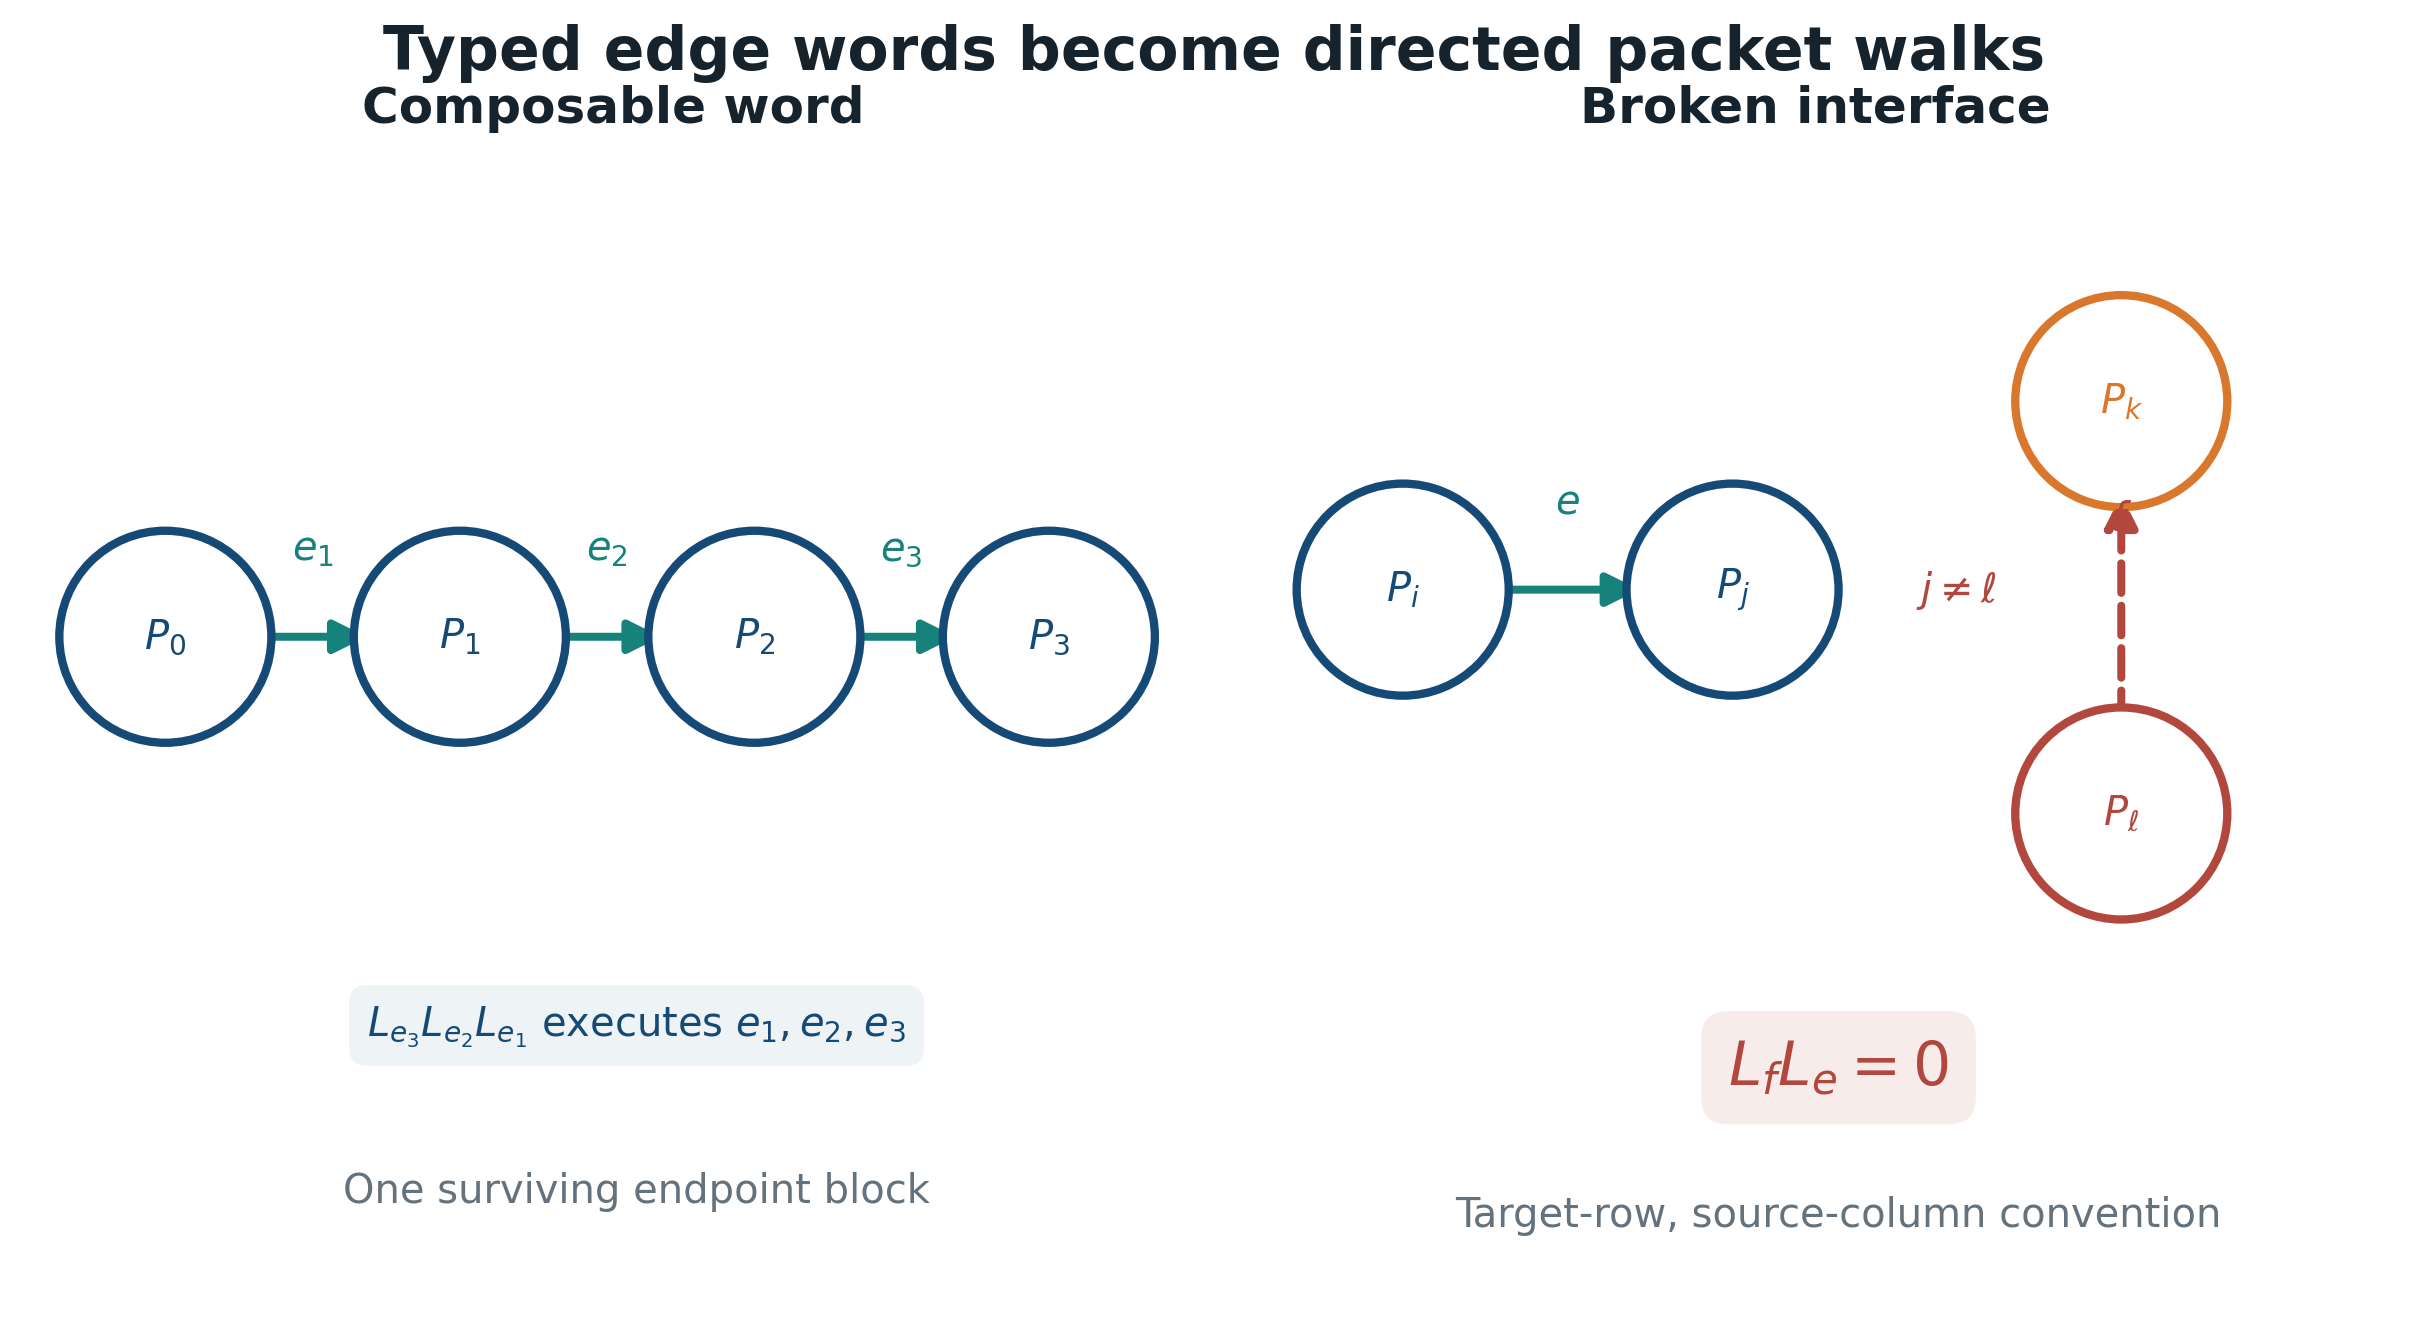
\includegraphics[width=0.98\linewidth]{typed_edge_walks.png}
\caption{The target-row, source-column convention fixes execution order.
Composable words collapse to endpoint blocks, while one broken packet
interface annihilates the entire operator product.}
\label{fig:typed-edge-walks}
\end{figure}

\section{Operator words and directed walks}
\label{sec:words-walks}

\subsection{Typed words}

\begin{definition}[Composable word and execution operator]
\label{def:word-op}
A finite word $w=(e_1,\ldots,e_n)$ is composable when
\[
  \tgt(e_r)=\src(e_{r+1})
  \qquad (1\le r<n).
\]
Set
\[
  L_w=L_{e_n}\cdots L_{e_1},
  \qquad L_{\varnothing}=I.
\]
This definition records the written order of execution even though matrix
composition is read right to left.
\end{definition}
\statusleanthree{Komorebi.PaperIII.EdgeOperators.PacketGraph.EdgeSystem.Composable; Komorebi.PaperIII.EdgeOperators.PacketGraph.EdgeSystem.wordOp}

\begin{theorem}[First broken interface]
\label{thm:first-break}
If a word begins $(e,f,\ldots)$ and $\tgt(e)\ne\src(f)$, then its word
operator is zero.
\end{theorem}
\statusleanthree{Komorebi.PaperIII.EdgeOperators.PacketGraph.EdgeSystem.wordOp_eq_zero_of_first_break}

\begin{theorem}[Nonwalk words vanish]
\label{thm:nonwalk-vanish}
If $w$ is not composable, then $L_w=0$.
\end{theorem}
\statusleanthree{Komorebi.PaperIII.EdgeOperators.PacketGraph.EdgeSystem.wordOp_eq_zero_of_not_composable}

\begin{proof}
Choose the first broken adjacent pair.  The corresponding consecutive factor
is zero by \cref{thm:edge-annihilation}, and associativity absorbs that zero
into the complete product.  The Lean proof implements the same argument by
induction on the list.
\end{proof}

\subsection{The checked recursive expansion}

\begin{definition}[Recursive word expansion]
\label{def:recursive-word-expansion}
Define
\[
  \cW_0=I,
  \qquad
  \cW_{n+1}=T\cW_n.
\]
\end{definition}
\statusleanthree{Komorebi.PaperIII.EdgeOperators.PacketGraph.EdgeSystem.wordExpansion}

\begin{theorem}[Transfer power equals recursive word expansion]
\label{thm:power-recursive-expansion}
For every $n\in\N$,
\[
  T^n=\cW_n.
\]
\end{theorem}
\statusleanthree{Komorebi.PaperIII.EdgeOperators.PacketGraph.EdgeSystem.transferOp_pow_eq_wordExpansion}

\begin{proof}
The zero case is the identity matrix.  If $T^n=\cW_n$, then the
left-successor power convention gives
$T^{n+1}=TT^n=T\cW_n=\cW_{n+1}$.
\end{proof}

\begin{remark}
The formal module also defines an explicit sum over tuples
$w:\operatorname{Fin}(n)\to E$ and a second sum in which noncomposable tuples
are replaced by zero.  It proves that the recursive, explicit, and
walk-filtered matrices agree.  These are separate declarations so that the
finite enumeration claim is auditable rather than hidden in the name
\emph{word expansion}.
\end{remark}
\statusleanthree{Komorebi.PaperIII.EdgeOperators.PacketGraph.EdgeSystem.explicitWordExpansion; Komorebi.PaperIII.EdgeOperators.PacketGraph.EdgeSystem.walkExpansion; Komorebi.PaperIII.EdgeOperators.PacketGraph.EdgeSystem.wordExpansion_eq_explicitWordExpansion; Komorebi.PaperIII.EdgeOperators.PacketGraph.EdgeSystem.explicitWordExpansion_eq_walkExpansion}

\subsection{Exact word-to-walk expansion}

For a nonempty composable word $w=(e_1,\ldots,e_n)$, define its reverse
coefficient product
\[
  c^\leftarrow(w)=c(e_n)c(e_{n-1})\cdots c(e_1).
\]
The reversal is essential over a noncommutative semiring.

\begin{lemma}[One word is one endpoint block]
\label{lem:word-endpoint}
If $w=(e_1,\ldots,e_n)$ is nonempty and composable, then
\[
  L_w
  =
  \operatorname{packetMatrix}
  \bigl(\src(e_1),\tgt(e_n);c^\leftarrow(w)\bigr).
\]
\end{lemma}
\statusleanthree{Komorebi.PaperIII.EdgeOperators.PacketGraph.EdgeSystem.reverseCoefficient; Komorebi.PaperIII.EdgeOperators.PacketGraph.EdgeSystem.terminalTarget; Komorebi.PaperIII.EdgeOperators.PacketGraph.EdgeSystem.wordOp_eq_packetMatrix_of_composable}

\begin{proof}
Induct on $n$.  The case $n=1$ is the definition of $L_e$.  Suppose the
formula holds for the prefix $(e_1,\ldots,e_n)$ and append $f$.  Composability
gives $\tgt(e_n)=\src(f)$.  Multiplying the two packet matrices leaves one
intermediate index and changes the coefficient to
$c(f)c(e_n)\cdots c(e_1)$, with source $\src(e_1)$ and target $\tgt(f)$.
\end{proof}

Write $\Walk_n(i,j)$ for the finite set of length-$n$ composable edge tuples
whose first source is $i$ and whose final target is $j$.  For $n=0$, it has
one empty walk when $i=j$ and is empty otherwise; assign the empty walk the
coefficient $1$.

\begin{theorem}[Finite operator word-to-walk expansion]
\label{thm:word-to-walk}
For every $n\in\N$,
\[
  \boxed{
  T^n
  =
  \sum_{w\in E^n}L_w
  =
  \sum_{w\in E^n}
  \begin{cases}
  L_w,&w\text{ composable},\\
  0,&w\text{ not composable}.
  \end{cases}
  }
\]
Parallel edges occur as distinct summands.
\end{theorem}
\statusleanthree{Komorebi.PaperIII.EdgeOperators.PacketGraph.EdgeSystem.transferOp_pow_eq_explicitWordExpansion; Komorebi.PaperIII.EdgeOperators.PacketGraph.EdgeSystem.transferOp_pow_eq_walkExpansion}

\begin{proof}
Induction and finite distributivity give
\[
\left(\sum_{e\in E}L_e\right)^n
=
\sum_{(e_1,\ldots,e_n)\in E^n}L_{e_n}\cdots L_{e_1}.
\]
Every noncomposable summand is zero by
\cref{thm:nonwalk-vanish}, so inserting the composability filter does not
change the sum.  In Lean, tuple concatenation and the successor sum are
handled by \leanname{tupleWordOp_snoc} and
\leanname{explicitWordExpansion_succ}; the two bridge equalities then yield
the displayed theorem.
\end{proof}

\begin{corollary}[Endpoint coefficient walk sum]
\label{cor:word-to-walk-entry}
For all $n\in\N$ and $i,j\in V$,
\[
  \boxed{
  (T^n)_{ji}
  =
  \sum_{w\in\Walk_n(i,j)}c^\leftarrow(w).
  }
\]
\end{corollary}
\statusleanthree{Komorebi.PaperIII.EdgeOperators.PacketGraph.EdgeSystem.Connects; Komorebi.PaperIII.EdgeOperators.PacketGraph.EdgeSystem.endpointWalkCoefficientSum; Komorebi.PaperIII.EdgeOperators.PacketGraph.EdgeSystem.transferOp_pow_apply_eq_sum_walks}

\begin{proof}
Take the $(j,i)$ entry in \cref{thm:word-to-walk}.  By
\cref{lem:word-endpoint}, a surviving word contributes
$c^\leftarrow(w)$ exactly when its endpoints are $i$ and $j$, and contributes
zero otherwise.  At $n=0$, the identity matrix gives the unique empty
diagonal walk.
\end{proof}

\begin{corollary}[Fixed-length reachability obstruction]
\label{cor:fixed-reachability}
If $\Walk_n(i,j)=\varnothing$, then $(T^n)_{ji}=0$.
\end{corollary}
\statusleanthree{Komorebi.PaperIII.EdgeOperators.PacketGraph.EdgeSystem.transferOp_pow_apply_eq_zero_of_no_walk}

\begin{proof}
This is immediate from the empty sum in the preceding corollary.
\end{proof}

\begin{corollary}[Orbit support obstruction]
\label{cor:orbit-reachability}
Let $S\subseteq V$, and let $x\in R^V$ be supported on $S$.  If $j$ is not
reachable by a directed path from any vertex of $S$, then
\[
  (T^nx)_j=0\qquad\text{for every }n\in\N.
\]
Hence the $T$-orbit of $x$ cannot generate a vector with nonzero
$j$-coordinate.
\end{corollary}
\statusleanthree{Komorebi.PaperIII.EdgeOperators.PacketGraph.EdgeSystem.Reachable; Komorebi.PaperIII.EdgeOperators.PacketGraph.EdgeSystem.transferOp_pow_mulVec_apply_eq_zero_of_unreachable_support}
\statusleanprior{Komorebi.PacketNaturalityCompletion.Reachability.algebraicOrbitHull_le_reachable_support; Komorebi.PacketNaturalityCompletion.Reachability.unreachable_nonzero_packet_obstruction}

\begin{proof}
Expand $(T^nx)_j=\sum_i(T^n)_{ji}x_i$.  Terms with $i\notin S$ vanish by
the support of $x$, and terms with $i\in S$ vanish by
\cref{cor:fixed-reachability}.  The final claim follows because the
$j$-coordinate also vanishes on every finite linear combination of orbit
vectors.
\end{proof}

\section{Canonical exact coordinate transport}
\label{sec:canonical-transport}

\subsection{The Paper III frame model}

Let every chart $a$ carry a linear frame equivalence
$F_a:M\xrightarrow{\sim}M$.  The formal Paper III module defines transport
from $a$ to $b$ by
\[
J_{b\leftarrow a}=F_b^{-1}F_a.
\]
This is the abstract frame form of \emph{synthesize in chart \(a\), then
analyze in chart \(b\)}.

\begin{theorem}[Exact frame transport is coherent]
\label{thm:exact-frame-transport}
For every $a,b,c$,
\[
J_{a\leftarrow a}=\id,\qquad
J_{a\leftarrow b}J_{b\leftarrow a}=\id,\qquad
J_{c\leftarrow b}J_{b\leftarrow a}=J_{c\leftarrow a},
\]
and therefore
\[
J_{a\leftarrow c}J_{c\leftarrow b}J_{b\leftarrow a}=\id.
\]
\end{theorem}
\statusleanthree{Komorebi.PaperIII.Transport.exactTransport_self; Komorebi.PaperIII.Transport.exactTransport_roundTrip; Komorebi.PaperIII.Transport.exactTransport_cocycle; Komorebi.PaperIII.Transport.exactTransport_triangleLoop}

\begin{proof}
Every identity is cancellation of adjacent $F_rF_r^{-1}$ factors.  The Lean
definitions use \leanname{LinearEquiv.trans}; the displayed formulas use the
equivalent right-to-left function-composition notation fixed in this paper.
\end{proof}

\begin{theorem}[Every finite canonical path telescopes]
\label{thm:exact-path-transport}
Let $p=(a_0,a_1,\ldots,a_n)$ be any finite vertex list and put
\[
J_p
=J_{a_n\leftarrow a_{n-1}}\cdots J_{a_1\leftarrow a_0},
\qquad
J_{(a_0)}=\id.
\]
Then
\[
J_p=J_{a_n\leftarrow a_0}.
\]
In particular, if $a_n=a_0$, then $J_p=\id$.
\end{theorem}
\statusleanthree{Komorebi.PaperIII.Transport.pathEndpoint; Komorebi.PaperIII.Transport.exactPathTransport; Komorebi.PaperIII.Transport.exactPathTransport_eq_endpoint; Komorebi.PaperIII.Transport.exactPathTransport_loop}

\begin{proof}
Induct on the list of successive vertices and apply the cocycle in
\cref{thm:exact-frame-transport} at each step.  If the endpoint is the start,
the endpoint transport is the identity.
\end{proof}

\subsection{Exact packet coordinates}

The graph model above resolves a fixed scalar matrix.  Coordinate transport
is a separate construction.  Let $X$ be an $R$-module, and let
\[
\cP^a=(P^a_i)_{i\in I_a}
\]
be a finite complete family of pairwise orthogonal linear idempotents:
\[
P^a_iP^a_j=\delta_{ij}P^a_i,
\qquad
\sum_{i\in I_a}P^a_i=I_X.
\]
Define the exact packet coordinate module
\[
\Coord(\cP^a)
=
\left\{(x_i)_{i\in I_a}:P^a_ix_i=x_i\right\}.
\]
Its analysis and synthesis maps are
\[
\cA_a(x)=(P^a_ix)_i,
\qquad
\cS_a((x_i)_i)=\sum_ix_i.
\]
Completeness and orthogonality give
\[
\cS_a\cA_a=\id_X,
\qquad
\cA_a\cS_a=\id_{\Coord(\cP^a)}.
\]

\begin{definition}[Canonical exact coordinate transport]
\label{def:canonical-J}
For two exact packet systems on the same ambient module, define
\[
  J^X_{b\leftarrow a}
  =
  \cA_b\cS_a:
  \Coord(\cP^a)\longrightarrow\Coord(\cP^b).
\]
The arrow points from the source coordinate system $a$ to the target
coordinate system $b$.
\end{definition}
\statusleanprior{Komorebi.PaperII.NestedRefinement.refineCoordinates; Komorebi.PaperII.NestedRefinement.coordinateRefinementEquiv}

\begin{theorem}[Identity, inverse, and cocycle for canonical transport]
\label{thm:J-cocycle}
For any exact packet systems $a,b,c$ on $X$,
\[
J^X_{a\leftarrow a}=\id,
\qquad
\left(J^X_{b\leftarrow a}\right)^{-1}=J^X_{a\leftarrow b},
\qquad
J^X_{c\leftarrow b}J^X_{b\leftarrow a}=J^X_{c\leftarrow a}.
\]
\end{theorem}
\statusleanprior{Komorebi.PaperII.NestedRefinement.refineCoordinates_self; Komorebi.PaperII.NestedRefinement.coarsenCoordinates_refineCoordinates; Komorebi.PaperII.NestedRefinement.refineCoordinates_coarsenCoordinates; Komorebi.PaperII.NestedRefinement.refineCoordinates_comp; Komorebi.PaperII.NestedRefinement.coordinateRefinementEquiv_trans}

\begin{proof}
Insert $\cS_b\cA_b=\id_X$:
\[
J^X_{c\leftarrow b}J^X_{b\leftarrow a}
=\cA_c\cS_b\cA_b\cS_a
=\cA_c\cS_a
=J^X_{c\leftarrow a}.
\]
The identity statement is $\cA_a\cS_a=\id$.  Setting $c=a$ in the cocycle
gives $J^X_{a\leftarrow b}J^X_{b\leftarrow a}=\id$; interchanging $a$ and $b$
gives the other composition, so the two transports are inverses.
\end{proof}

If $F:X\to Y$ is linear and $\cP^a,\cP^b$ are source packet systems while
$\cQ^r,\cQ^s$ are target packet systems, put
\[
\widehat F_{r\leftarrow a}
=
\cA^Y_rF\cS^X_a.
\]

\begin{theorem}[Canonical coordinate naturality]
\label{thm:canonical-naturality}
The exact coordinate representation preserves typed composition and satisfies
\[
J^Y_{s\leftarrow r}\widehat F_{r\leftarrow a}
=
\widehat F_{s\leftarrow b}J^X_{b\leftarrow a}.
\]
\end{theorem}
\statusleanprior{Komorebi.PaperII.NestedRefinement.coordinateOperator_comp; Komorebi.PaperII.NestedRefinement.coordinateOperator_naturality}

\begin{proof}
Both sides reduce to $\cA^Y_sF\cS^X_a$ after inserting the appropriate
synthesis--analysis identity.  The composition law is the same calculation
with the middle ambient module inserted.
\end{proof}

\begin{corollary}[Canonical triangle holonomy is trivial]
\label{cor:J-flat}
For every triple $a,b,c$,
\[
J^X_{a\leftarrow c}J^X_{c\leftarrow b}J^X_{b\leftarrow a}=\id.
\]
\end{corollary}
\statusleanprior{Komorebi.PaperII.NestedRefinement.refineCoordinates_comp; Komorebi.PaperII.NestedRefinement.refineCoordinates_self}

\begin{boundary}[Refinement is not reduction]
Although Paper II uses the name \emph{refineCoordinates}, $J$ is an
equivalence between two complete coordinate presentations.  It neither
truncates packets nor projects to a smaller state space.  Any lossy
restriction, interpolation, or learned identification is extra data and
cannot inherit \cref{thm:J-cocycle} without proof.
\end{boundary}

\section{A distinct noncanonical connection API}
\label{sec:connection}

\subsection{The minimal compiled API}

The formal Paper III API starts with deliberately weak assumptions.  All
chart transports act on one module $M$, so chart labels distinguish routes
but not Lean types.

\begin{definition}[Self-normalized noncanonical connection]
\label{def:minimal-connection}
A minimal connection is a family
\[
\Gamma_{b\leftarrow a}\in\operatorname{Aut}_R(M)
\qquad(a,b\in B)
\]
with only
\[
\Gamma_{a\leftarrow a}=\id_M.
\]
Neither reverse-edge inversion nor the cocycle law is a field of the
structure.
\end{definition}
\statusleanthree{Komorebi.PaperIII.Transport.Connection}

At a triple $(a,b,c)$, the compiled cocycle predicate is
\[
\Gamma_{c\leftarrow b}\Gamma_{b\leftarrow a}
=\Gamma_{c\leftarrow a}.
\]
Flatness means this equality holds for every triple.  The formal
multiplicative relative defect and triangle holonomy are
\[
D^\times_{c,b,a}
=
\bigl(\Gamma_{c\leftarrow b}\Gamma_{b\leftarrow a}\bigr)
\Gamma_{c\leftarrow a}^{-1},
\qquad
H_{c,b,a}
=
\Gamma_{a\leftarrow c}
\Gamma_{c\leftarrow b}
\Gamma_{b\leftarrow a}.
\]
The defect is based at the target $c$; the holonomy is based at $a$.
\statusleanthree{Komorebi.PaperIII.Transport.Connection.CocycleAt; Komorebi.PaperIII.Transport.Connection.Flat; Komorebi.PaperIII.Transport.Connection.cocycleDefect; Komorebi.PaperIII.Transport.Connection.triangleHolonomy}

\begin{theorem}[Checked flatness consequences]
\label{thm:minimal-flatness}
For the minimal connection API, flatness implies
\[
D^\times_{c,b,a}=\id_M,
\qquad
H_{c,b,a}=\id_M
\]
for every $a,b,c$.
\end{theorem}
\statusleanthree{Komorebi.PaperIII.Transport.Connection.cocycleDefect_eq_refl_of_flat; Komorebi.PaperIII.Transport.Connection.triangleHolonomy_eq_refl_of_flat}

\begin{proof}
Flatness replaces the two-edge route in $D^\times$ by the direct route,
which cancels its inverse.  For $H$, flatness first collapses $a\to b\to c$
to $a\to c$, then collapses $a\to c\to a$ to the normalized transport
$a\to a$.
\end{proof}

\begin{proposition}[The minimal API admits nontrivial holonomy]
\label{prop:twisted-loop}
There is a connection on three points over $\mathbb Q$ for which transport
$0\to1$ is multiplication by $2$, every other unequal-endpoint transport is
the identity, and
\[
H_{2,1,0}(1)=2.
\]
In particular $H_{2,1,0}\ne\id$.
\end{proposition}
\statusleanthree{Komorebi.PaperIII.Transport.twistedThreePointConnection; Komorebi.PaperIII.Transport.twisted_triangleHolonomy_apply_one; Komorebi.PaperIII.Transport.twisted_triangleHolonomy_ne_refl}

\begin{boundary}[Why the minimal defect and loop are distinct]
Without reverse-edge inversion,
$\Gamma_{a\leftarrow c}$ need not equal
$\Gamma_{c\leftarrow a}^{-1}$.  Therefore the multiplicative relative defect
$D^\times_{c,b,a}$ and triangle holonomy $H_{c,b,a}$ are different
comparisons.  The formal module proves that global flatness trivializes both;
it does not identify them for an arbitrary connection.
\end{boundary}

\begin{figure}[H]
\centering
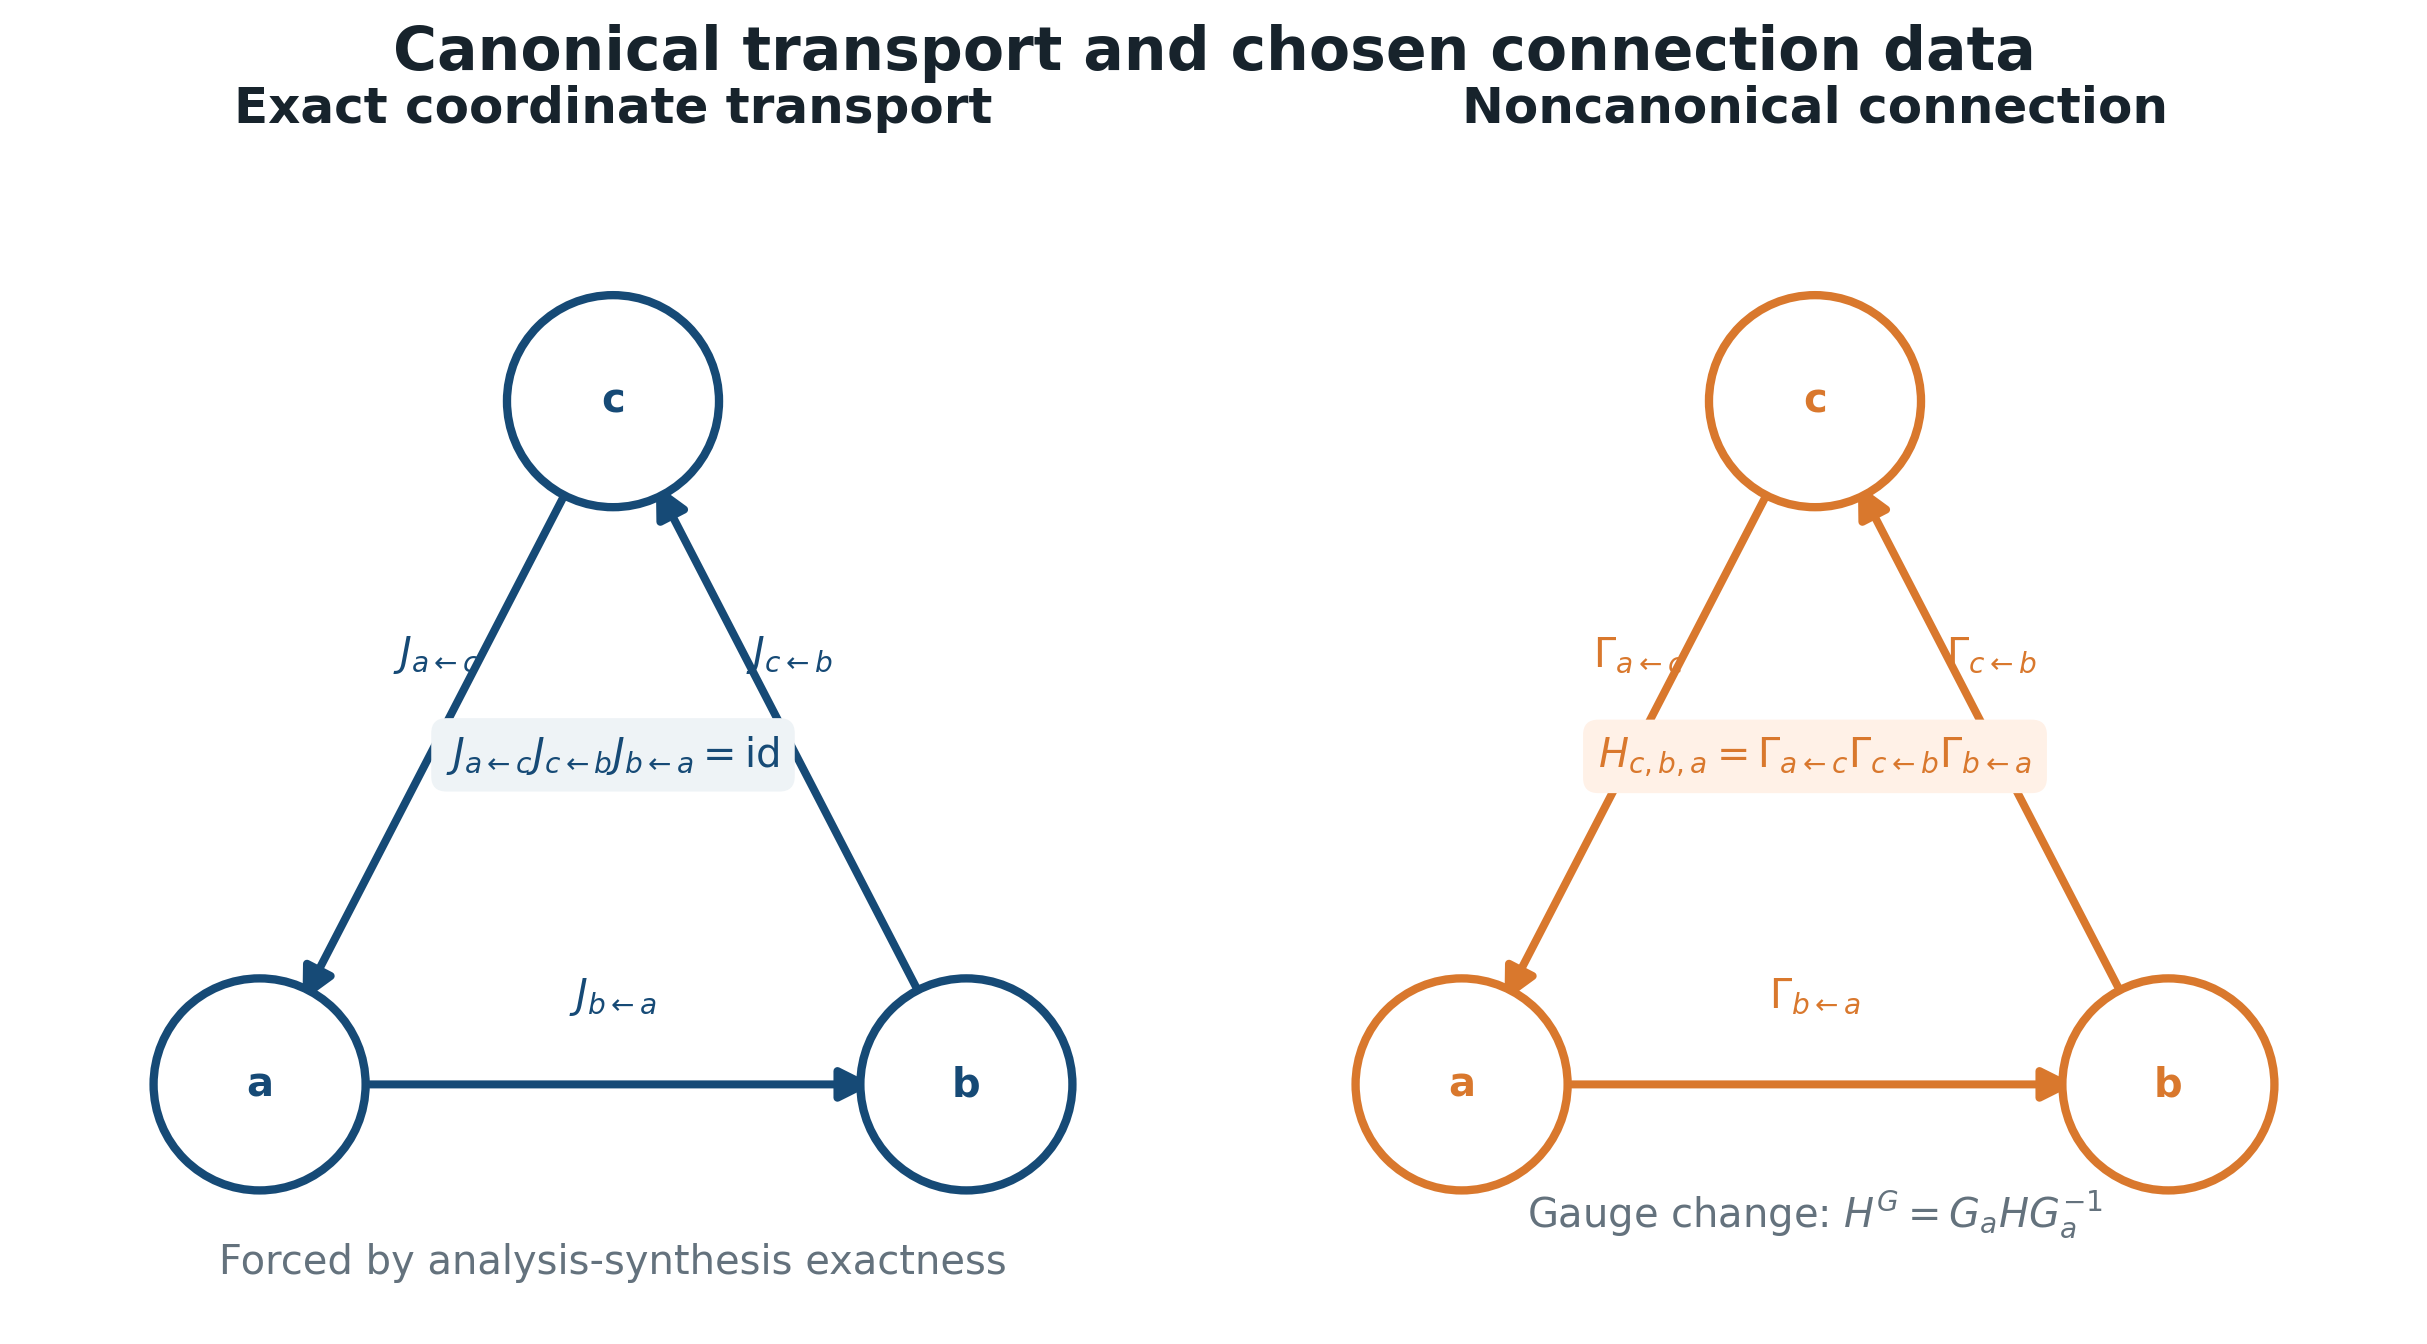
\includegraphics[width=0.98\linewidth]{transport_vs_connection.png}
\caption{Exact coordinate transport and connection transport are distinct.
The canonical loop telescopes to the identity.  A chosen connection may
carry nontrivial holonomy, which transforms by conjugation under gauge.}
\label{fig:transport-connection}
\end{figure}

\Cref{fig:transport-connection} records this separation visually: the exact
coordinate route telescopes, whereas the chosen connection route may carry a
nonidentity loop.

\subsection{A stronger reversible pair API}

Let $R$ be a commutative ring, let $B$ be a type of charts or refinement
states, and let each $C_a$ be an $R$-module.  The chart type is not assumed
finite.  The following definition is deliberately not derived from analysis
and synthesis.

\begin{definition}[Normalized reversible connection]
\label{def:connection}
A normalized reversible connection is a family of linear equivalences
\[
\Gamma_{b\leftarrow a}:C_a\xrightarrow{\;\sim\;}C_b
\qquad(a,b\in B)
\]
such that
\[
\Gamma_{a\leftarrow a}=\id,
\qquad
\Gamma_{a\leftarrow b}=\Gamma_{b\leftarrow a}^{-1}.
\]
No cocycle equation is included in the structure.
\end{definition}
\statusleanthree{Komorebi.PaperIII.Transport.ReversibleConnection}

This strengthens the homogeneous minimal connection with heterogeneous
fibers and reverse-edge inversion.  It remains additional data, not an alias
for canonical coordinate transport.

\begin{definition}[Calibration and flatness]
\label{def:calibration-flatness}
When the $C_a$ are exact packet coordinates of one ambient module, the
connection is \emph{canonically calibrated} if
\[
\Gamma_{b\leftarrow a}=J_{b\leftarrow a}
\quad\text{for every }a,b.
\]
It is \emph{flat} if
\[
\Gamma_{c\leftarrow b}\Gamma_{b\leftarrow a}
=
\Gamma_{c\leftarrow a}
\quad\text{for every }a,b,c.
\]
The canonical connection is flat; a general flat connection is proved in
\cref{thm:flat-gauge-canonical} to be gauge-equivalent to it.
\end{definition}
\statusleanthree{Komorebi.PaperIII.Transport.ReversibleConnection.CocycleAt; Komorebi.PaperIII.Transport.ReversibleConnection.Flat; Komorebi.PaperIII.Transport.ReversibleConnection.canonicalConnection; Komorebi.PaperIII.Transport.ReversibleConnection.canonicalConnection_flat}

The words \emph{calibrated} and \emph{flat} have only the algebraic meanings
displayed above.

\begin{remark}[Graph-local variant]
One may specify $\Gamma_e$ only on the oriented edges of a chart graph,
together with inverse maps on reversed edges.  Path transport and loop
holonomy below still make sense.  A direct cocycle defect for $(a,b,c)$,
however, requires a declared direct transport from $a$ to $c$.  The pairwise
API in \cref{def:connection} keeps this comparison total.
\end{remark}

\subsection{Cocycle defect and triangle holonomy}

The commutative-ring hypothesis makes subtraction of linear maps available
from this point through \cref{sec:obstruction-packets}.

\begin{definition}[Cocycle defect]
\label{def:cocycle-defect}
For $a,b,c\in B$, define the additive cocycle defect
\[
\Delta_{c,b,a}
=
\Gamma_{c\leftarrow b}\Gamma_{b\leftarrow a}
-\Gamma_{c\leftarrow a}
\in\Hom_R(C_a,C_c).
\]
\end{definition}
\statusleanthree{Komorebi.PaperIII.Transport.ReversibleConnection.cocycleDefect}

The manuscript subscript order is target, intermediate, source.  The Lean
arguments are supplied in traversal order \leanname{(a,b,c)}.

\begin{definition}[Triangle holonomy]
\label{def:triangle-holonomy}
The triangle holonomy based at $a$ is
\[
H_{c,b,a}
=
\Gamma_{a\leftarrow c}
\Gamma_{c\leftarrow b}
\Gamma_{b\leftarrow a}
\in\operatorname{Aut}_R(C_a).
\]
It traverses $a\to b\to c\to a$.
\end{definition}
\statusleanthree{Komorebi.PaperIII.Transport.ReversibleConnection.triangleHolonomy; Komorebi.PaperIII.Transport.ReversibleConnection.triangleObstruction}

Holonomy is attached to the chosen connection $\Gamma$, never to an
unspecified coordinate change.

\begin{theorem}[Defect--holonomy identity]
\label{thm:defect-holonomy}
For every triple $(a,b,c)$,
\[
\boxed{
H_{c,b,a}-\id_{C_a}
=
\Gamma_{a\leftarrow c}\Delta_{c,b,a}.
}
\]
Consequently,
\[
\Delta_{c,b,a}=0
\quad\Longleftrightarrow\quad
H_{c,b,a}=\id_{C_a}.
\]
\end{theorem}
\statusleanthree{Komorebi.PaperIII.Transport.ReversibleConnection.triangleHolonomy_sub_id; Komorebi.PaperIII.Transport.ReversibleConnection.cocycleDefect_eq_zero_iff_triangleHolonomy_eq_refl}

\begin{proof}
Using reversibility,
\[
\begin{aligned}
\Gamma_{a\leftarrow c}\Delta_{c,b,a}
&=
\Gamma_{a\leftarrow c}
\Gamma_{c\leftarrow b}
\Gamma_{b\leftarrow a}
-
\Gamma_{a\leftarrow c}\Gamma_{c\leftarrow a}\\
&=H_{c,b,a}-\id_{C_a}.
\end{aligned}
\]
Left composition by the equivalence $\Gamma_{a\leftarrow c}$ is injective,
which gives the equivalence of the two vanishing statements.
\end{proof}

\begin{corollary}[Canonical transport has zero connection defect]
\label{cor:canonical-zero-defect}
If $\Gamma_{b\leftarrow a}=J_{b\leftarrow a}$, then
\[
\Delta_{c,b,a}=0,
\qquad
H_{c,b,a}=\id
\]
for all triples.
\end{corollary}
\statusleanthree{Komorebi.PaperIII.Transport.ReversibleConnection.canonicalTransport_zero_connectionDefect; Komorebi.PaperIII.Transport.ReversibleConnection.canonicalTransport_triangleHolonomy_eq_refl}

\begin{proof}
The defect vanishes by the canonical cocycle in
\cref{thm:J-cocycle}; apply \cref{thm:defect-holonomy}.
\end{proof}

\subsection{Paths and endpoint independence}

\begin{definition}[Path-ordered connection transport]
\label{def:path-transport}
For a vertex sequence
$p=(a_0,a_1,\ldots,a_n)$, define
\[
\Gamma_p
=
\Gamma_{a_n\leftarrow a_{n-1}}\cdots
\Gamma_{a_1\leftarrow a_0},
\qquad
\Gamma_{(a_0)}=\id_{C_{a_0}}.
\]
If $a_n=a_0$, then $\Gamma_p$ is the holonomy of the loop $p$.
\end{definition}
\statusleanthree{Komorebi.PaperIII.Transport.ReversibleConnection.pathTransport; Komorebi.PaperIII.Transport.ReversibleConnection.VertexPath; Komorebi.PaperIII.Transport.ReversibleConnection.indexedPathTransport}

Products are path-ordered: the first traversed edge acts on the right.

\begin{proposition}[Flat pair transport collapses to endpoints]
\label{prop:flat-endpoints}
If $\Gamma$ is flat, then every path satisfies
\[
\Gamma_p=\Gamma_{a_n\leftarrow a_0}.
\]
In particular, every loop has identity holonomy.
\end{proposition}
\statusleanthree{Komorebi.PaperIII.Transport.ReversibleConnection.pathTransport_eq_direct_of_flat; Komorebi.PaperIII.Transport.ReversibleConnection.indexedPathTransport_eq_direct_of_flat; Komorebi.PaperIII.Transport.ReversibleConnection.indexedLoopTransport_eq_refl_of_flat}

\begin{proof}
Induct on the path length.  Appending $a_{n+1}$ left-multiplies the
inductive expression by $\Gamma_{a_{n+1}\leftarrow a_n}$, and flatness
replaces the two factors by
$\Gamma_{a_{n+1}\leftarrow a_0}$.  For a loop, normalization gives
$\Gamma_{a_0\leftarrow a_0}=\id$.
\end{proof}

\begin{remark}
The converse \emph{trivial holonomy implies flatness} depends on which loops
are present in a graph-local API.  In the complete pair API, triviality of
every triangle holonomy is equivalent to flatness by
\cref{thm:defect-holonomy}.  No topological simple-connectivity theorem is
being invoked.
\end{remark}

\section{Gauge covariance and comparison with canonical transport}
\label{sec:gauge}

\begin{definition}[Gauge change]
\label{def:gauge-change}
A gauge is a family of automorphisms $G_a\in\operatorname{Aut}_R(C_a)$.
It acts on a connection by
\[
\Gamma^G_{b\leftarrow a}
=
G_b\Gamma_{b\leftarrow a}G_a^{-1}.
\]
\end{definition}
\statusleanthree{Komorebi.PaperIII.Transport.ReversibleConnection.Gauge; Komorebi.PaperIII.Transport.ReversibleConnection.gauge}

A gauge changes coordinate representatives at each chart; it does not change
the chart graph.

\begin{theorem}[Gauge covariance]
\label{thm:gauge-covariance}
The defect and triangle holonomy transform as
\[
\Delta^G_{c,b,a}
=G_c\Delta_{c,b,a}G_a^{-1},
\qquad
H^G_{c,b,a}
=G_aH_{c,b,a}G_a^{-1}.
\]
Thus flatness and triviality of triangle holonomy are gauge invariant.
\end{theorem}
\statusleanthree{Komorebi.PaperIII.Transport.ReversibleConnection.gauge_cocycleDefect; Komorebi.PaperIII.Transport.ReversibleConnection.gauge_triangleHolonomy; Komorebi.PaperIII.Transport.ReversibleConnection.gauge_flat_iff; Komorebi.PaperIII.Transport.ReversibleConnection.gauge_triangleHolonomy_eq_refl_iff}

\begin{proof}
Substitute the definition of $\Gamma^G$.  Adjacent factors
$G_b^{-1}G_b$ and $G_c^{-1}G_c$ cancel.  In the defect, both the composite
and direct terms acquire the same outer factors $G_c$ and $G_a^{-1}$.  In
the loop, all inner factors cancel and only conjugation at the base remains.
\end{proof}

\begin{theorem}[Flat connections are gauges of the canonical pair transport]
\label{thm:flat-gauge-canonical}
Suppose the $C_a$ are exact packet-coordinate modules for one ambient module,
so the canonical $J_{b\leftarrow a}$ is available.  If $\Gamma$ is a flat
normalized reversible pair connection, choose $o\in B$ and set
\[
G_a=\Gamma_{a\leftarrow o}J_{o\leftarrow a}.
\]
Then every pair transport satisfies
\[
\boxed{
\Gamma_{b\leftarrow a}
=G_bJ_{b\leftarrow a}G_a^{-1}.
}
\]
\end{theorem}
\statusleanthree{Komorebi.PaperIII.Transport.ReversibleConnection.flatGauge; Komorebi.PaperIII.Transport.ReversibleConnection.flat_isGaugeOfCanonical}

\begin{proof}
Reversibility gives
$G_a^{-1}=J_{a\leftarrow o}\Gamma_{o\leftarrow a}$.  Therefore
\[
\begin{aligned}
G_bJ_{b\leftarrow a}G_a^{-1}
&=
\Gamma_{b\leftarrow o}
J_{o\leftarrow b}J_{b\leftarrow a}
J_{a\leftarrow o}
\Gamma_{o\leftarrow a}\\
&=
\Gamma_{b\leftarrow o}\Gamma_{o\leftarrow a}\\
&=
\Gamma_{b\leftarrow a}.
\end{aligned}
\]
The first reduction uses the canonical cocycle twice; the second uses
flatness of $\Gamma$.
\end{proof}

\begin{boundary}[Flat does not mean calibrated]
The theorem produces a gauge relating $\Gamma$ to $J$.  It does not prove
$\Gamma=J$ before that gauge is chosen.  Conversely, nontrivial triangle
holonomy cannot be removed by a gauge, because conjugation cannot turn a
nonidentity automorphism into the identity.
\end{boundary}

\section{Obstruction packets: local certificates and holonomy blocks}
\label{sec:obstruction-packets}

\subsection{The generic compiled certificate}

Let $\mathsf{Candidate}$, $\mathsf{Packet}$, and $\mathsf{Residual}$ be
arbitrary types, with a distinguished
$0\in\mathsf{Residual}$, and let
\[
r:\mathsf{Candidate}\longrightarrow
\mathsf{Packet}\longrightarrow\mathsf{Residual}
\]
be a residual function.

\begin{definition}[Candidate-specific solution and obstruction packet]
\label{def:generic-obstruction}
A candidate $x$ is a solution when
\[
\operatorname{IsSolution}_r(x)
\quad\Longleftrightarrow\quad
\forall p,\ r(x,p)=0.
\]
An obstruction packet for $x$ is a pair consisting of a named packet $p$
and a certificate $r(x,p)\ne0$.
\end{definition}
\statusleanthree{Komorebi.PaperIII.NonlinearObstructions.IsSolution; Komorebi.PaperIII.NonlinearObstructions.ObstructionPacket}

\begin{theorem}[Exact logical force of a local obstruction]
\label{thm:generic-obstruction}
Every obstruction packet for $x$ proves that $x$ is not a solution, and
\[
\neg\operatorname{IsSolution}_r(x)
\quad\Longleftrightarrow\quad
\text{there exists an obstruction packet for }x.
\]
The reverse implication from failure to a packet witness is classical and
does not require the packet type to be finite.
\end{theorem}
\statusleanthree{Komorebi.PaperIII.NonlinearObstructions.ObstructionPacket.not_isSolution; Komorebi.PaperIII.NonlinearObstructions.obstructionPacket_of_not_isSolution; Komorebi.PaperIII.NonlinearObstructions.not_isSolution_iff_nonempty_obstructionPacket}

\begin{proof}
A purported solution would make the residual vanish at the certified packet,
contradicting its nonzero field.  Conversely, if no packet carries a nonzero
residual, then every residual is zero and the candidate satisfies the
definition of solution.
\end{proof}

\begin{boundary}[Candidate-specific means candidate-specific]
The theorem rules out the named $x$.  It neither constructs a solution nor
shows that every candidate is obstructed.  It provides no minimality,
stability, computability, or classification theorem for the packet witness.
\end{boundary}

\subsection{Holonomy-block specialization}

For a reversible connection, the generic residual may be specialized at a
fixed triangle by taking a packet label to be a pair $(\mu,\nu)$ and the
residual to be the corresponding block of $H-\id$.  A block is therefore a
packet residual; when it is nonzero, the label together with a proof of
nonvanishing is an obstruction-packet certificate in the sense of
\cref{def:generic-obstruction}.  The reconstruction theorem below is the extra
statement needed to turn vanishing of all those local residuals into the
cocycle equation at that triangle.

Fix a triangle $(a,b,c)$ and resolve the base fiber $C_a$ by a finite complete
family of idempotents $(\Pi^a_\mu)_{\mu\in I_a}$.  Orthogonality may also hold,
as it does for the exact range-coordinate projectors below, but the compiled
reconstruction theorem does not require it.  In exact range coordinates,
$\Pi^a_\mu$ is simply the projector that retains component $\mu$ and zeros
the other components.

\begin{definition}[Holonomy obstruction and packet residuals]
\label{def:obstruction-packet}
Define
\[
\Ob_{c,b,a}=H_{c,b,a}-\id_{C_a},
\qquad
\Ob^{\mu\nu}_{c,b,a}
=
\Pi^a_\mu\Ob_{c,b,a}\Pi^a_\nu.
\]
The map $\Ob^{\mu\nu}_{c,b,a}$ is the obstruction block, or packet residual,
from input packet $\nu$ to output packet $\mu$.  If it is nonzero, then
$(\mu,\nu)$ and that nonvanishing proof form an obstruction-packet
certificate.  Diagonal blocks detect within-packet holonomy; off-diagonal
blocks detect holonomy-induced packet mixing.
\end{definition}
\statusleanthree{Komorebi.PaperIII.HolonomyBlocks.PacketResolution; Komorebi.PaperIII.HolonomyBlocks.PacketResolution.block}

An obstruction-packet certificate here is a nonzero block of a precisely
specified holonomy defect together with its packet-pair label; it is not
merely a heuristic label for a large residual.

\begin{theorem}[Exact obstruction-block reconstruction and detection]
\label{thm:obstruction-detection}
The total obstruction has the exact finite resolution
\[
\boxed{
\Ob_{c,b,a}
=
\sum_{\mu,\nu\in I_a}
\Ob^{\mu\nu}_{c,b,a}.
}
\]
Moreover, the following are equivalent:
\begin{enumerate}[label=(\roman*)]
\item $\Delta_{c,b,a}=0$;
\item $H_{c,b,a}=\id$;
\item $\Ob_{c,b,a}=0$;
\item $\Ob^{\mu\nu}_{c,b,a}=0$ for every $\mu,\nu$.
\end{enumerate}
\end{theorem}
\statusleanthree{Komorebi.PaperIII.HolonomyBlocks.obstruction_sum_blocks; Komorebi.PaperIII.HolonomyBlocks.obstructionBlocks_zero_iff; Komorebi.PaperIII.HolonomyBlocks.obstructionDetection_equivalences}

\begin{proof}
Insert completeness on both sides:
\[
\Ob
=
\left(\sum_\mu\Pi^a_\mu\right)
\Ob
\left(\sum_\nu\Pi^a_\nu\right)
=
\sum_{\mu,\nu}\Pi^a_\mu\Ob\Pi^a_\nu.
\]
Thus (iv) implies (iii), and (iii) implies (iv) by composition with the
projectors.  Conditions (ii) and (iii) are equivalent by the definition of
$\Ob$ and additive cancellation.
Conditions (i) and (ii) are equivalent by
\cref{thm:defect-holonomy}.
\end{proof}

\Cref{fig:holonomy-obstruction-blocks} depicts the two-sided finite block
resolution behind the reconstruction identity and its off-diagonal witnesses.

\begin{figure}[H]
\centering
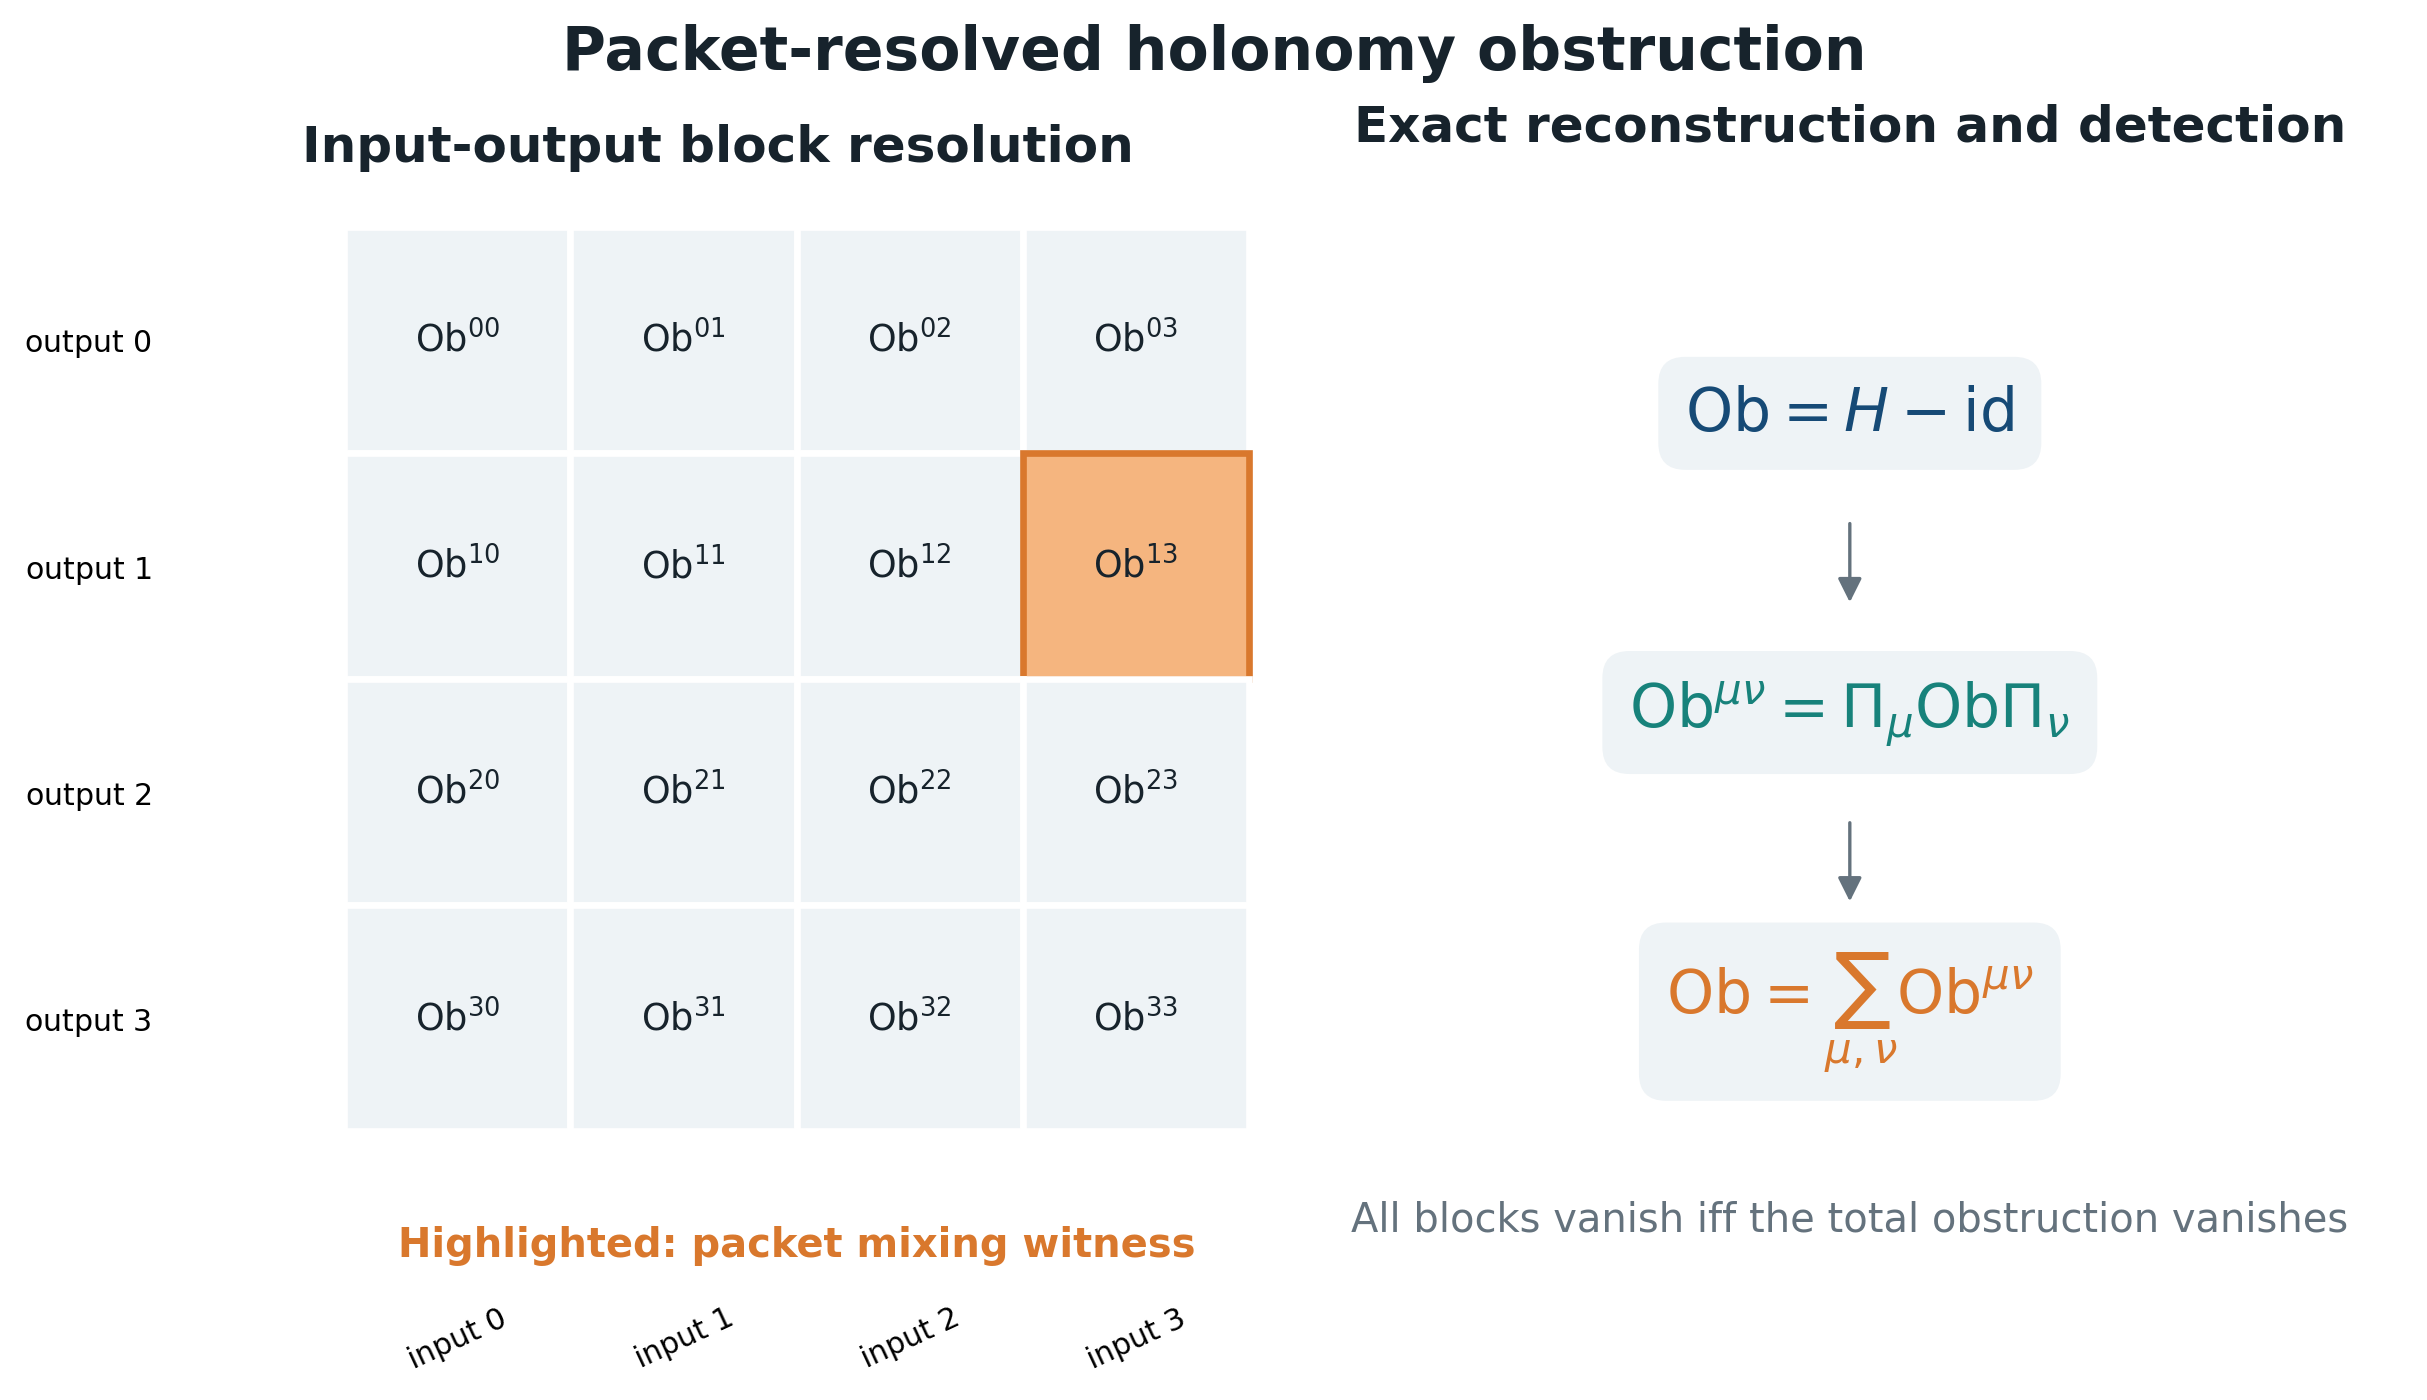
\includegraphics[width=0.98\linewidth]{holonomy_obstruction_blocks.png}
\caption{A finite complete packet resolution reconstructs the total holonomy
obstruction from its input-output blocks.  A nonzero off-diagonal block is an
exact packet-mixing witness.}
\label{fig:holonomy-obstruction-blocks}
\end{figure}

\begin{corollary}[Packet-supported witness]
\label{cor:packet-witness}
If $\Ob^{\mu\nu}_{c,b,a}\ne0$, then there is a vector $x$ supported in packet
$\nu$ such that
\[
\Pi^a_\mu\Ob_{c,b,a}x\ne0.
\]
Such an $x$ is an exact finite witness of nonflatness.
\end{corollary}
\statusleanthree{Komorebi.PaperIII.HolonomyBlocks.exists_packetWitness_of_obstructionBlock_ne_zero}

\begin{proof}
Classically choose $y$ on which the nonzero linear map
$\Pi^a_\mu\Ob\Pi^a_\nu$ is nonzero and set $x=\Pi^a_\nu y$.
Idempotence gives $\Pi^a_\nu x=x$, and the required output is the chosen
nonzero value.
\end{proof}

\subsection{Gauge behavior of packet blocks}

Vanishing or nonvanishing of the total triangle obstruction is gauge invariant
by \cref{thm:gauge-covariance}, but a fixed packet pattern need not be.  A
general $G_a$ can mix the projectors $\Pi^a_\mu$.

\begin{proposition}[Packet-preserving gauge covariance]
\label{prop:packet-gauge}
If $G_a\Pi^a_\mu=\Pi^a_\mu G_a$ for every $\mu$, then
\[
\left(\Ob^G\right)^{\mu\nu}
=
G_a\Ob^{\mu\nu}G_a^{-1}.
\]
Consequently the zero/nonzero status of each obstruction block is preserved
by packet-preserving gauges.
\end{proposition}
\statusleanthree{Komorebi.PaperIII.HolonomyBlocks.obstructionBlock_gauge_of_commutes; Komorebi.PaperIII.HolonomyBlocks.obstructionBlock_gauge_eq_zero_iff}

\begin{proof}
Use $\Ob^G=G_a\Ob G_a^{-1}$ and commute $G_a$ and $G_a^{-1}$ through the
two packet projectors.  Composition by an equivalence is injective in both
directions.
\end{proof}

\begin{boundary}[Packet patterns are not absolute]
Without the commutation hypothesis in \cref{prop:packet-gauge}, only the
vanishing of the total obstruction is gauge invariant.  The location of
individual nonzero blocks may change under a gauge that mixes packets.
\end{boundary}

\section{Packet-supported products and holonomy walks}
\label{sec:holonomy-walks}

The word-to-walk mechanism is not special to powers of one matrix.  Let $V$
be one finite packet type, let $R$ be a semiring, and let
$B_1,\ldots,B_m\in R^{V\times V}$ be a finite sequence of possibly different
packet matrices.  Rows are targets and columns are sources as before.

\begin{proposition}[Heterogeneous packet-path expansion]
\label{prop:heterogeneous-path}
For $i,j\in V$ and $m\geq1$, set $i_0=i$ and $i_m=j$.  Then
\[
\boxed{
(B_m\cdots B_1)_{ji}
=
\sum_{(i_1,\ldots,i_{m-1})\in V^{m-1}}
  B_m[i_m,i_{m-1}]\cdots B_1[i_1,i_0].
}
\]
When $m=1$, the sum is over the unique empty tuple and its summand is
$B_1[j,i]$.
For $m=0$, the product is the identity and the entry is the Kronecker delta
$\delta_{ji}$.  If every $B_r[q,p]$ vanishes outside a declared relation
$\mathcal R_r(p,q)$, then the endpoint entry is zero whenever there is no
packet path compatible with the successive relations.
\end{proposition}
\statusleanthree{Komorebi.PaperIII.EdgeOperators.heterogeneousProduct; Komorebi.PaperIII.EdgeOperators.heterogeneousPathSum; Komorebi.PaperIII.EdgeOperators.heterogeneousPacketPathExpansion; Komorebi.PaperIII.EdgeOperators.SupportedStep; Komorebi.PaperIII.EdgeOperators.SupportedPath; Komorebi.PaperIII.EdgeOperators.heterogeneousProduct_apply_eq_zero_of_no_supportedPath}

\begin{proof}
Expand each matrix product entry and distribute the finite sums.  Induction on
the factor list yields the displayed path sum, with the empty list evaluated
as the identity matrix.  If no supported intermediate packet exists, every
summand contains an entry that is zero by its declared support relation.
\end{proof}

\begin{boundary}[Changing packet types along a chain]
The compiled theorems
\leanname{heterogeneousPacketPathExpansion_two} and
\leanname{heterogeneousPacketPathExpansion_three} allow different packet
types at the successive stages of two- and three-factor products.  The
arbitrary-length theorem above permits different factors but uses one common
finite packet type $V$.  A fully dependent arbitrary-length chain of changing
modules and packet types remains outside the version 1.0.1 contract.
\end{boundary}

\begin{remark}[Checked specialization]
When every $B_r$ is one repeated endomorphism $T$, the recursive packet-power
specialization is inherited from Paper I.
\end{remark}
\statusleanprior{Komorebi.PacketNaturalityCompletion.Packets.transferBlock_pow_eq_packetPathSum}

For a loop represented on one common finite scalar packet-coordinate type,
the proposition resolves its successive transport matrices into packet
walks.  If $R$ is a ring, as in the reversible-connection API, then
$(H-I)_{ji}=H_{ji}-\delta_{ji}$; in particular, off-diagonal entries are
unchanged.  Thus a nonzero off-diagonal holonomy obstruction in this
common-index model requires a transport word along the closed chart loop
whose packet path runs from its input packet to its output packet.  This
conclusion is conditional on declared block supports for the connection
matrices; an arbitrary connection need not respect the transfer graph from
\cref{sec:edge-operators}.

\section{A minimal exact example}
\label{sec:example}

\begin{example}[A scalar triangle]
Let $B=\{0,1,2\}$ and $C_0=C_1=C_2=\bbk$ for a field $\bbk$.  Choose
$u,v,w\in\bbk^\times$ and set
\[
\Gamma_{1\leftarrow0}(x)=ux,\qquad
\Gamma_{2\leftarrow1}(x)=vx,\qquad
\Gamma_{2\leftarrow0}(x)=wx,
\]
with reverse transports given by inverse scalars.  Then
\[
\Delta_{2,1,0}(x)=(vu-w)x,
\]
and the triangle holonomy based at $0$ is
\[
H_{2,1,0}(x)=w^{-1}vux.
\]
Therefore
\[
H_{2,1,0}-\id
=w^{-1}\Delta_{2,1,0}.
\]
The connection is flat on this triangle exactly when $vu=w$.  If the three
coordinate systems are literally the same and canonical transport is used,
then $u=v=w=1$ and the obstruction vanishes.  Choosing arbitrary nonzero
$u,v,w$ is a connection choice, not a consequence of changing exact packet
coordinates.
\end{example}

\begin{example}[A two-step transfer walk]
Let a packet graph have edges $e:0\to1$ and $f:1\to2$, with no other edges.
Then
\[
T=L_e+L_f,\qquad
(T^2)_{20}=c(f)c(e).
\]
The products $L_eL_e$, $L_eL_f$, and $L_fL_f$ vanish by typed mismatch;
only $L_fL_e$, corresponding to the walk $0\to1\to2$, contributes to the
$(2,0)$ entry.  This example also fixes the noncommutative coefficient order.
\end{example}

\section{Canonical coordinates for arbitrary maps}
\label{sec:arbitrary-maps}

The analysis and synthesis identities are identities of functions, not only
of linear maps.  Consequently exact coordinate change does not become
curved merely because the represented operation is nonlinear.

\begin{proposition}[Set-level exact naturality]
\label{prop:set-naturality}
Let $\cA^X_a:X\xrightarrow{\sim}X_a$ and
$\cA^X_b:X\xrightarrow{\sim}X_b$ be exact coordinate equivalences for $X$,
with inverses $\cS^X_a$ and $\cS^X_b$.  Likewise, let
$\cA^Y_r:Y\xrightarrow{\sim}Y_r$ and
$\cA^Y_s:Y\xrightarrow{\sim}Y_s$ be exact coordinate equivalences for $Y$,
with inverses $\cS^Y_r$ and $\cS^Y_s$.  Let $F:X\to Y$ be any function, with
no linearity or differentiability hypothesis.  Set
\[
J^X_{b\leftarrow a}=\cA^X_b\circ\cS^X_a,
\qquad
J^Y_{s\leftarrow r}=\cA^Y_s\circ\cS^Y_r,
\]
and define
\[
\widehat F_{r\leftarrow a}
=
\cA^Y_r\circ F\circ\cS^X_a.
\]
Then
\[
J^Y_{s\leftarrow r}\circ\widehat F_{r\leftarrow a}
=
\widehat F_{s\leftarrow b}\circ J^X_{b\leftarrow a}.
\]
If $\cA^Z_t:Z\xrightarrow{\sim}Z_t$ is another exact coordinate equivalence
and $G:Y\to Z$ is any function, then exact coordinate representation also
preserves composition:
\[
\widehat{G\circ F}_{t\leftarrow a}
=
\widehat G_{t\leftarrow r}\circ\widehat F_{r\leftarrow a}.
\]
\end{proposition}
\statusleanthree{Komorebi.PaperIII.Transport.exactCoordinateMap; Komorebi.PaperIII.Transport.exactCoordinateMap_comp; Komorebi.PaperIII.Transport.exactCoordinateMap_naturality}

\begin{proof}
Both sides of the naturality equation reduce to
$\cA^Y_s\circ F\circ\cS^X_a$ using
$\cS\circ\cA=\id$ in $X$ and $Y$.  For composition, the middle
$\cS^Y\circ\cA^Y$ cancels in the same way.
\end{proof}

\begin{boundary}[Where nonlinear defects can enter]
A nonlinear \emph{coordinate} defect cannot be blamed on the exact canonical
$J$ of \cref{def:canonical-J}; \cref{prop:set-naturality} makes that defect
identically zero.  Nonzero defects require extra structure such as a
noncanonical connection, truncation, approximation, restricted domains, or
failure of an operation to respect a declared packet model.
\end{boundary}

\clearpage\section{Nonlinear operation trees: locality and the formalization frontier}
\label{sec:operation-trees}

\subsection{The compiled unary--binary foundation}

\begin{definition}[Finite operation-tree grammar]
\label{def:compiled-operation-tree}
For types of input labels $I$, constants $K$, unary symbols $U$, and binary
symbols $B$, the released formal grammar has four constructors:
\[
\begin{aligned}
t ::={}&\operatorname{input}(i)
\mid\operatorname{constant}(k)
\mid\operatorname{unary}(u,t)\\
&\mid\operatorname{binary}(b,t_1,t_2).
\end{aligned}
\]
Given an arbitrary value type $Y$, evaluation takes completely explicit maps
\[
I\to Y,\qquad K\to Y,\qquad U\to Y\to Y,\qquad
B\to Y\to Y\to Y.
\]
No algebraic, continuity, or differentiability law is imposed on these
semantics.
\end{definition}
\statusleanthree{Komorebi.PaperIII.NonlinearObstructions.OperationTree; Komorebi.PaperIII.NonlinearObstructions.OperationTree.eval}

When $I$ has decidable equality, let $\operatorname{inputs}(t)$ be the finite
set of input labels actually occurring in $t$.

\begin{theorem}[Operation-tree input locality]
\label{thm:tree-locality}
Let $\eta_1,\eta_2:I\to Y$ be two input environments.  If
\[
\eta_1(i)=\eta_2(i)
\qquad\text{for every }i\in\operatorname{inputs}(t),
\]
then the two evaluations of $t$ are equal under the same constant, unary, and
binary semantics.  In particular, if
$\operatorname{inputs}(t)=\varnothing$, evaluation is independent of the
input environment.
\end{theorem}
\statusleanthree{Komorebi.PaperIII.NonlinearObstructions.OperationTree.eval_congr_on_inputs; Komorebi.PaperIII.NonlinearObstructions.OperationTree.eval_eq_of_inputs_eq_empty}

\begin{proof}
Structural induction on $t$.  The input case is the agreement hypothesis;
the constant case is reflexive; the unary case applies the induction
hypothesis to its child; and the binary case applies it independently to the
left and right subtrees, whose input sets form a union.
\end{proof}

\begin{boundary}[Exact force of locality]
The theorem says evaluation reads only syntactically named inputs.  It does
not prove that the operations are linear or nonlinear in any analytic sense,
that the tree is stable, that two different trees are equivalent, or that a
solution to a tree equation exists.
\end{boundary}

\subsection{Typed colored extension beyond the finite contract}

\begin{definition}[Finitary colored operation signature]
\label{def:signature}
A finitary colored signature consists of:
\begin{itemize}
\item a finite type $V$ of colors;
\item a type $\Sigma$ of operation symbols;
\item an arity $r(\sigma)\in\N$ for every $\sigma\in\Sigma$;
\item input colors
$\operatorname{in}_\sigma:\operatorname{Fin}(r(\sigma))\to V$;
\item an output color $\operatorname{out}(\sigma)\in V$.
\end{itemize}
A realization assigns a space $X_v$ to each color and a map
\[
\Phi_\sigma:
\prod_{q\in\operatorname{Fin}(r(\sigma))}X_{\operatorname{in}_\sigma(q)}
\longrightarrow X_{\operatorname{out}(\sigma)}.
\]
\end{definition}
\statusroadmap{The intended Lean target is a dependent inductive typed tree; no such declaration is part of the version 1.0.1 completion contract.}

\begin{definition}[Typed operation tree and evaluation]
\label{def:operation-tree}
A typed operation tree is recursively either a leaf of declared color or a
node labeled by $\sigma$, with one correctly colored child for each input
slot of $\sigma$.  Evaluation is recursive:
\[
\ev(\operatorname{node}(\sigma;t_1,\ldots,t_{r(\sigma)}))
=
\Phi_\sigma(\ev(t_1),\ldots,\ev(t_{r(\sigma)})).
\]
\end{definition}
\statusroadmap{Candidate API: \leanname{Komorebi.PaperIII.NonlinearObstructions.ColoredOperationTree} and \leanname{ColoredOperationTree.eval}.  This is stronger than the compiled uncolored unary--binary grammar.}

\subsection{Packet labelings and the multilinear first target}

Suppose every $X_v$ has a finite complete packet family
$(P^v_i)_{i\in I_v}$.  A packet labeling assigns an admissible packet index
to each edge or node of a typed tree.  For multilinear $\Phi_\sigma$, inserting
\[
\id_{X_v}=\sum_{i\in I_v}P^v_i
\]
at every input and output yields a finite sum over packet-labeled trees.
This is the branching analogue of inserting intermediate projectors in
\cref{prop:heterogeneous-path}.

\begin{roadmap}[Finite multilinear tree expansion]
\label{roadmap:multilinear-tree}
The first milestone for the nonlinear module is an exact theorem saying that the
evaluation of a finite tree of multilinear nodes equals the finite sum of its
packet-resolved labeled evaluations.  Required proof obligations include:
\begin{enumerate}[label=(\alph*)]
\item a dependent well-typed tree syntax;
\item finite packet-label types at every color;
\item an explicit convention for nullary and unary nodes;
\item multilinearity in every input slot;
\item preservation of input-slot order without assuming commutativity of
operations.
\end{enumerate}
\end{roadmap}
\statusroadmap{Candidate target: \leanname{Komorebi.PaperIII.NonlinearObstructions.ColoredOperationTree.eval_eq_sum_packetLabellings}.}

\subsection{Connection defects at nonlinear nodes}

For coordinate models of the source and target colors, an additive target
coordinate space, and a chosen noncanonical connection, a pointwise node
defect can be defined by
\[
\mathfrak D^\Gamma_{b,a}(\Phi)
=
\Gamma^Y_{b\leftarrow a}\circ\widehat\Phi_a
-
\widehat\Phi_b\circ
\left(\prod_q\Gamma^{X_q}_{b\leftarrow a}\right).
\]
This expression compares two \emph{chosen} routes.  With canonical exact
transport in every slot it vanishes by \cref{prop:set-naturality}.

\begin{roadmap}[Operation-tree defect propagation]
\label{roadmap:tree-defect}
For multilinear nodes, one expects an exact finite expansion obtained by
replacing one or more nodes by their defects and transporting the remaining
branches.  For smooth nonlinear nodes, the corresponding chain rule is
indexed by rooted partitions and Fa\`a di Bruno trees.  A formal theorem will
require a fixed differentiability category, base points, derivative
conventions, symmetry factors, and remainder policy.
\end{roadmap}
\statusroadmap{Tree-level defect identities, higher chain rules, and nonlinear norm bounds are outside the finite Lean contract. Ordinary mathematical results in these directions appear in Part~II under their stated hypotheses.}

\begin{boundary}[Analytic and geometric exclusions]
The finite formal contract does not include convergence of an infinite tree series, existence
of derivatives, a Banach-space Fa\`a di Bruno theorem, a Baker--Campbell--Hausdorff
expansion, a continuum limit, or an identification of algebraic holonomy with
curvature of a smooth bundle. Part~II supplies ordinary proofs for its explicit nonlinear and analytic statements. This edition does not derive a connection from
data, optimization, physics, or probability.
\end{boundary}

\section{Formalization ledger for version 1.0.1}
\label{sec:ledger}

\small
\begin{longtable}{L{0.17\textwidth}L{0.18\textwidth}L{0.25\textwidth}L{0.22\textwidth}}
\toprule
Topic & Status & Declaration or roadmap target & Exact boundary\\
\midrule
\endfirsthead
\toprule
Topic & Status & Declaration or roadmap target & Exact boundary\\
\midrule
\endhead
Packet matrix and edge operator
& Lean-backed III
& \leanname{PacketGraph.packetMatrix}; \leanname{EdgeSystem.edgeOp}
& Finite scalar matrices over a semiring; one scalar coordinate per packet.\\
\addlinespace
Edge support and pair dichotomy
& Lean-backed III
& \leanname{edgeOp_eq_zero_off_support}; \leanname{edgeOp_mul_edgeOp_eq_zero}; \leanname{edgeOp_mul_edgeOp_of_composable}
& Broken interfaces vanish; matched pairs collapse to the endpoint block with coefficient in operator order.\\
\addlinespace
Typed word evaluation
& Lean-backed III
& \leanname{Composable}; \leanname{wordOp}; \leanname{wordOp_append}; \leanname{wordOp_eq_zero_of_not_composable}
& List order is execution order; concatenation reverses operator-product order; nonwalks vanish.\\
\addlinespace
Finite word and walk expansions
& Lean-backed III
& \leanname{explicitWordExpansion}; \leanname{walkExpansion}; \leanname{wordExpansion_eq_explicitWordExpansion}; \leanname{transferOp_pow_eq_walkExpansion}
& Actual finite tuple sum and zero-filtered composable-walk sum; finite graph and packet types.\\
\addlinespace
Endpoint coefficient walk sum
& Lean-backed III
& \leanname{reverseCoefficient}; \leanname{Connects}; \leanname{transferOp_pow_apply_eq_sum_walks}
& Exact scalar endpoint entry, including the empty-walk case and noncommutative coefficient order.\\
\addlinespace
Fixed reachability and orbit support
& Lean-backed III; inherited hull bridge
& \leanname{transferOp_pow_apply_eq_zero_of_no_walk}; \leanname{transferOp_pow_mulVec_apply_eq_zero_of_unreachable_support}
& Finite powers and supported seeds; the orbit-hull span conclusion uses the frozen Paper I contract.\\
\addlinespace
Exact frame transport
& Lean-backed III
& \leanname{exactTransport_cocycle}; \leanname{exactPathTransport_eq_endpoint}; \leanname{exactPathTransport_loop}
& One frame family on a single module; arbitrary finite paths telescope and closed paths are trivial.\\
\addlinespace
Exact coordinate cocycle
& Inherited Lean-backed II
& \leanname{NestedRefinement.refineCoordinates_comp}; \leanname{NestedRefinement.coordinateRefinementEquiv_trans}
& Complete finite projector coordinates, not reduction.\\
\addlinespace
Typed coordinate naturality
& Inherited Lean-backed II
& \leanname{NestedRefinement.coordinateOperator_comp}; \leanname{NestedRefinement.coordinateOperator_naturality}
& Linear maps over semiring modules.\\
\addlinespace
Minimal connection API
& Lean-backed III
& \leanname{Transport.Connection}; \leanname{cocycleDefect}; \leanname{triangleHolonomy}; \leanname{triangleHolonomy_eq_refl_of_flat}
& Only self-normalization is assumed; reverse inversion and the cocycle are not structure fields.\\
\addlinespace
Twisted three-point loop
& Lean-backed III
& \leanname{twistedThreePointConnection}; \leanname{twisted_triangleHolonomy_ne_refl}
& Concrete rational connection; the selected loop sends \(1\) to \(2\).\\
\addlinespace
Reversible additive defect
& Lean-backed III
& \leanname{ReversibleConnection}; \leanname{triangleHolonomy_sub_id}; \leanname{cocycleDefect_eq_zero_iff_triangleHolonomy_eq_refl}
& Heterogeneous module fibers, reverse-edge inversion, and an additive defect over a commutative ring.\\
\addlinespace
Reversible finite paths
& Lean-backed III
& \leanname{pathTransport_eq_direct_of_flat}; \leanname{indexedPathTransport_eq_direct_of_flat}; \leanname{indexedLoopTransport_eq_refl_of_flat}
& Finite pair-connection paths collapse to endpoints under algebraic flatness.\\
\addlinespace
Gauge covariance
& Lean-backed III
& \leanname{gauge_cocycleDefect}; \leanname{gauge_triangleHolonomy}; \leanname{gauge_flat_iff}
& Fiberwise algebraic conjugation; no smooth gauge theory.\\
\addlinespace
Flat versus canonical transport
& Lean-backed III
& \leanname{flatGauge}; \leanname{flat_isGaugeOfCanonical}
& A chosen base chart and ambient frames exhibit every flat pair connection as a gauge transform of canonical transport.\\
\addlinespace
Operation-tree locality
& Lean-backed III
& \leanname{OperationTree}; \leanname{OperationTree.eval}; \leanname{OperationTree.eval_congr_on_inputs}
& Arbitrary unary and binary semantics; only dependence on named inputs is proved.\\
\addlinespace
Generic obstruction packet
& Lean-backed III
& \leanname{ObstructionPacket.not_isSolution}; \leanname{not_isSolution_iff_nonempty_obstructionPacket}
& Exact candidate-specific logical certificate; no global classification.\\
\addlinespace
Holonomy block obstruction
& Lean-backed III
& \leanname{obstruction_sum_blocks}; \leanname{obstructionBlocks_zero_iff}; \leanname{obstructionDetection_equivalences}
& Finite complete idempotent packet family on the base fiber; orthogonality is not required by the compiled reconstruction.\\
\addlinespace
Packet witness and block gauge
& Lean-backed III
& \leanname{exists_packetWitness_of_obstructionBlock_ne_zero}; \leanname{obstructionBlock_gauge_of_commutes}; \leanname{obstructionBlock_gauge_eq_zero_iff}
& Witness extraction is classical; blockwise covariance requires the gauge to commute with every packet projector.\\
\addlinespace
Heterogeneous matrix paths
& Lean-backed III
& \leanname{heterogeneousPacketPathExpansion}; \leanname{heterogeneousProduct_apply_eq_zero_of_no_supportedPath}
& Arbitrarily many different matrices over one common finite packet type; fully typed changing-index chains compile only at lengths two and three.\\
\addlinespace
Arbitrary-function coordinates
& Lean-backed III
& \leanname{exactCoordinateMap_comp}; \leanname{exactCoordinateMap_naturality}
& Exact set-level equivalences and arbitrary functions; no linearity or differentiability assumption.\\
\addlinespace
Colored and smooth trees
& Roadmap only
& roadmap \leanname{ColoredOperationTree.eval_eq_sum_packetLabellings}
& Dependent colors, multilinear packet expansion, derivatives, and Fa\`a di Bruno identities remain outside the contract.\\
\bottomrule
\end{longtable}
\normalsize

\subsection{Kernel-backed Paper III surface}

The authoritative declaration-level contract is
\path{formalization/lean/LEAN_THEOREM_MAP_v1.0.1.md}.  It groups the compiled
surface as follows.
\begin{itemize}
\item \textbf{EdgeOperators and EdgeExtensions:} scalar packet matrices,
typed edge and word support, finite word/walk expansions, endpoint coefficient
sums, fixed-length reachability, orbit support, and common-index
heterogeneous products with declared supports.
\item \textbf{Transport and ReversibleConnections:} exact frame transport,
the minimal connection, heterogeneous reversible pair transport, additive
defect and triangle holonomy, finite paths, canonical connections, and the
fiberwise gauge action.
\item \textbf{CoordinateNaturality and HolonomyBlocks:} composition and
naturality for arbitrary functions between exact coordinate systems, finite
two-sided block reconstruction, equivalent obstruction criteria,
packet-supported witnesses, and packet-preserving block gauges.
\item \textbf{NonlinearObstructions:} finite unary--binary operation trees,
input locality, and candidate-specific obstruction certificates.
\end{itemize}
The release verification report records the checker-generated declaration
and audit totals.  The parity gate requires every fully qualified Paper III
target printed beside a statement to occur in the theorem map, rejects stale
or duplicate targets, and checks it against the compiled environment.
\path{KernelAudit.lean} reports dependencies for the mapped and supporting
theorems, and its fail-closed gate scans every compiled
\leanname{Komorebi.PaperIII} declaration.  The four inherited statement
contracts remain identified separately by their Papers I--II names.

\begin{boundary}[No scope promotion by prose]
The displayed endpoint coefficient formula, reachability results, reversible
connection theorems, additive defect--holonomy identity, gauge covariance,
holonomy-block reconstruction, packet witnesses, common-index heterogeneous
path expansion, and arbitrary-function coordinate naturality are all part of
the version 1.0.1 kernel-backed surface.  What remains outside is the
dependent fiber-valued edge-system generalization, a fully dependent
arbitrary-length chain whose module and packet type change at every stage,
dependent colored operation trees, packet-labeled multilinear tree
expansions, nonlinear tree-defect and Fa\`a di Bruno identities, and the
analytic and geometric extensions listed above.
\end{boundary}

\section{The finite contract and the nonlinear transition}

Typed packet support turns the expansion of a transfer power into a walk
calculus: incompatible words vanish for structural reasons, not because of
numerical cancellation.  Exact packet-coordinate transport is even more
rigid.  It is the canonical analysis--synthesis equivalence and therefore
satisfies its cocycle law exactly; every finite canonical loop telescopes to
the identity.  Holonomy enters only after a separate connection is supplied.
The kernel-backed minimal API proves that flatness kills both the relative
defect and holonomy, and it exhibits a nontrivial rational loop.  Under the
kernel-backed reversible API, a nonzero additive triangle defect is equivalent to nonidentity
holonomy, transforms covariantly under gauge, and is detected exactly by a
finite family of packet blocks.  Finite flat paths collapse to their endpoints,
and every flat reversible pair connection is explicitly gauge-equivalent to
canonical transport through a chosen base chart.

These facts define the boundary of the finite formal contract.  At that
boundary, exact coordinates preserve composition and satisfy naturality for
arbitrary functions in Paper III, while the typed linear packet-coordinate
counterpart remains inherited from Paper~II.  Nontrivial nonlinear defects
must therefore be attached to additional modeling choices or to
operation-specific packet compatibility.  Colored operation trees,
multilinear packet labelings, and Fa\`a di Bruno expansions remain
outside this finite Lean contract. Part~II develops the corresponding ordinary mathematics, including packet jets, rooted tree expansions, and explicit nonlinear obstruction theorems.


\clearpage
\part{Nonlinear packet calculus, obstruction complexes, and holonomy}\label{part:nonlinear}
\noindent The strengthened development below moves from exact arbitrary-function coordinates to differentiable interactions, specified correction problems, and finite or smooth transport. Its ordinary proofs retain their own hypotheses. They are not asserted to belong to the finite Lean contract of Part~I.

\medskip\noindent The notational change from \(\cA,\cS\) to \(\Acal,\Scal\) is typographical: both denote analysis and synthesis for the declared packet system. A connection is still additional data. Smooth canonical transport is constructed from a moving projector family, whereas the algebraic exact coordinate transport in Part~I compares fixed exact descriptions of one ambient object.
\section{Introduction}\label{sec:introduction}

A finite family of pairwise annihilating idempotents gives exact coordinates.  If
\[
P_\alpha P_\beta=0
\quad\text{for }\alpha\ne\beta,
\qquad
\sum_\alpha P_\alpha=I,
\]
then every vector is the sum of its packet components.  Linear operators become block matrices in these coordinates.  A nonlinear map cannot be reconstructed from its diagonal restrictions, since mixed interactions between packet components are usually present.  It can still be represented exactly if its input is the complete packet tuple.

This article develops the nonlinear representation and the obstruction theory that follows from it.  Exact coordinates preserve a nonlinear problem, but they do not solve it.  Once the equation is written in packet coordinates, its derivatives, compositions, correction maps, refinement failures, and gluing defects can be separated without discarding mixed terms.

The first stage of Part~II treats the local nonlinear calculus.  Packet analysis and synthesis conjugate arbitrary maps.  Fr\'echet derivatives split into multilinear packet jets.  The higher chain rule then becomes a Fa\`a di Bruno formula whose terms carry intermediate packet labels.  Standard background on Fr\'echet calculus and the higher chain rule may be found in \cite{AbrahamMarsdenRatiu1988,ConstantineSavits1996,Deimling1985}.

The next stage studies nonlinear iteration.  Repeated substitution is indexed by rooted trees rather than operator words.  A scalar majorant gives an absolute convergence theorem for polynomial fixed point equations.  The quadratic case recovers the Catalan series.  Rooted tree combinatorics are discussed in \cite{Stanley2012,LodayVallette2012,HairerLubichWanner2006}.

The correction stage concerns correction and obstruction.  A linear correction map
\[
D:U\longrightarrow V
\]
places the obstruction to solving $Du=-r$ in the canonical quotient $\coker D$.  This quotient has a universal property and behaves naturally under commuting squares.  Mapping cones extend the same construction to cochain complexes.  In a Hilbert space with closed range, the quotient is represented by the orthogonal projection onto $\Ker D^*$.  The Moore Penrose inverse then gives the least norm correction.  Relevant background appears in \cite{Weibel1994,Penrose1955}.

A vanishing linear obstruction is only the first step.  We give a contraction theorem for nonlinear correction, followed by a local Lyapunov Schmidt reduction.  In a complete filtered problem, every lifting step has its own cokernel class.  Vanishing at all depths and compatible choices of corrections produce an exact inverse limit solution.  A filtered correction complex carries a spectral sequence.  Its first page records graded obstruction candidates, while later differentials record interactions that can cancel them.  We use the standard spectral sequence of a filtered complex from \cite{Weibel1994,McCleary2001}.

The final stage studies elimination and gluing.  The implicit function theorem gives an exact Schur derivative after hidden variables are removed.  Finite transport systems reduce, after a spanning tree gauge, to one holonomy element for each fundamental cycle.  The same idea extends to smooth projector families through Kato transport.  We use standard material from \cite{Deimling1985,GrossTucker1987,Kato1950,Kato1995,KobayashiNomizu1963}.

The article does not claim that every nonlinear problem has a finite obstruction space.  The cokernel is canonical only after a correction map has been specified.  It may be infinite dimensional.  A first order obstruction may vanish while a higher order obstruction remains.  The purpose of the calculus is to identify the exact object in which each failure lives and to show how those objects change under packets, refinement, filtration, and transport.


\section{A map of the nonlinear calculus}\label{sec:map}

Four different questions recur throughout the paper.  They should not be merged into one vague idea of nonlinear structure.

The first question is representation.  Given a nonlinear map $F$, can its packet form be written without approximation?  The answer is yes.  Analysis and synthesis are inverse coordinate maps, so conjugation preserves the full equation.

The second question is interaction.  Which input packets influence a given output packet, and at what derivative order?  Packet jets answer this question.  They form a directed hypergraph rather than an ordinary block matrix because one nonlinear interaction can have several inputs.

The third question is correction.  Suppose an approximate solution leaves a defect $r$.  A declared linearized correction map $D$ removes the part of $r$ lying in $\im D$.  The quotient class
\[
[r]\in\coker D
\]
is the part that no allowed first order correction can remove.  This is the obstruction.  A nonlinear theorem is still needed after that class vanishes.

The fourth question is gluing.  Local coordinate changes can solve every edge problem and still fail around a loop.  The remaining cycle product is holonomy.  It is an obstruction to one global frame, not an obstruction to solving a single local equation.

These four layers fit into the sequence
\[
\begin{gathered}
\text{exact coordinates}
\longrightarrow
\text{packet interactions}
\longrightarrow
\text{correction classes}
\\
\longrightarrow
\text{global gluing}.
\end{gathered}
\]
Each arrow needs hypotheses.  Exact coordinates need a complete packet system.  Differential interactions need regularity.  A cokernel obstruction needs a specified correction map.  Holonomy needs invertible local transports.

A second distinction concerns scale.  A refinement defect compares a fine nonlinear model with a coarse one.  It is a point in the coarse output space.  An obstruction class is the image of such a defect, or of another residual, in a quotient by allowed corrections.  The two are related only after the correction map has been declared.  A small defect can have a nonzero obstruction, and a large defect can have zero obstruction if it lies entirely in the correction range.

The paper uses finite packet systems in the coordinate and graph sections.  Banach space hypotheses enter only where norms, contractions, or Fr\'echet derivatives are used.  Module and complex language is used for cokernels, filtered lifting, and cohomological obstructions.  This separation keeps each result at the level of generality supported by its proof.

\subsection*{Standing conventions}
All packet systems are finite unless a statement says otherwise.  In a normed setting every packet projector and every coarsening operator is bounded.  Differentiability of operator valued maps is taken in operator norm.  A Banach space isomorphism is a bounded linear bijection with bounded inverse.  For a decreasing filtration $(F^mX)$, completeness means that the canonical map
\[
X\longrightarrow\varprojlim_m X/F^mX
\]
is an isomorphism and separatedness means $\bigcap_mF^mX=0$.  Statements about congruence classes in a filtered nonlinear problem also assume that the nonlinear map preserves filtration congruences at the stated depth.  These assumptions are repeated where they are essential to a proof.

\section{Exact nonlinear packet coordinates}\label{sec:nonlinear_coordinates}

Let $X$ be a module over a unital ring.  A finite packet system on $X$ is a family
\[
\Pcal=(P_\alpha)_{\alpha\in I}\subseteq\End(X)
\]
of nonzero idempotents such that
\[
P_\alpha P_\beta=0
\quad\text{when }\alpha\ne\beta,
\qquad
\sum_{\alpha\in I}P_\alpha=I_X.
\]
Write
\[
X_\alpha=P_\alpha X,
\qquad
X^{\Pcal}=\bigoplus_{\alpha\in I}X_\alpha.
\]
The analysis and synthesis maps are
\[
\Acal_{\Pcal}x=(P_\alpha x)_\alpha,
\qquad
\Scal_{\Pcal}(x_\alpha)_\alpha=\sum_\alpha x_\alpha.
\]
They are inverse isomorphisms.

\begin{definition}[Nonlinear packet coordinate map]\label{def:nonlinear_packet_map}
Let $\Pcal$ be a packet system on $X$ and let $\Qcal$ be a packet system on $Y$.  For any map $F:X\to Y$, define
\[
F_{\Qcal\leftarrow\Pcal}
=
\Acal_{\Qcal}F\Scal_{\Pcal}.
\]
Thus
\[
F_{\Qcal\leftarrow\Pcal}((x_\alpha)_\alpha)
=
\left(
Q_\gamma F\left(\sum_\alpha x_\alpha\right)
\right)_\gamma.
\]
\end{definition}

\begin{theorem}[Exact nonlinear coordinate theorem]\label{thm:exact_nonlinear_coordinates}
For every map $F:X\to Y$,
\[
\Scal_{\Qcal}F_{\Qcal\leftarrow\Pcal}\Acal_{\Pcal}=F.
\]
If $G:Y\to Z$ and $\Rcal$ is a packet system on $Z$, then
\[
(G\circ F)_{\Rcal\leftarrow\Pcal}
=
G_{\Rcal\leftarrow\Qcal}
\circ
F_{\Qcal\leftarrow\Pcal}.
\]
No linearity, continuity, or differentiability assumption is needed.
\end{theorem}

\begin{proof}
The identities $\Scal_{\Pcal}\Acal_{\Pcal}=I_X$ and $\Scal_{\Qcal}\Acal_{\Qcal}=I_Y$ give
\[
\Scal_{\Qcal}F_{\Qcal\leftarrow\Pcal}\Acal_{\Pcal}
=
\Scal_{\Qcal}\Acal_{\Qcal}F\Scal_{\Pcal}\Acal_{\Pcal}
=F.
\]
For composition,
\[
G_{\Rcal\leftarrow\Qcal}F_{\Qcal\leftarrow\Pcal}
=
\Acal_{\Rcal}G\Scal_{\Qcal}\Acal_{\Qcal}F\Scal_{\Pcal}
=
\Acal_{\Rcal}(G\circ F)\Scal_{\Pcal}.
\]
\end{proof}

\begin{corollary}[Dynamical equivalence]\label{cor:dynamical_equivalence}
Suppose $X=Y$ and the same packet system is used on both sides.  Packet coordinates preserve fixed points, periodic points, injectivity, surjectivity, and invertibility.  In particular,
\[
F(x)=x
\quad\Longleftrightarrow\quad
F_{\Pcal\leftarrow\Pcal}(\Acal_{\Pcal}x)=\Acal_{\Pcal}x.
\]
\end{corollary}

\begin{proof}
The packet map is conjugate to $F$ through the isomorphism $\Acal_{\Pcal}$.  Every listed property is invariant under conjugacy.
\end{proof}

\begin{proposition}[Change of packet coordinates]\label{prop:change_packet_coordinates}
Let $\Pcal$ and $\Pcal'$ be packet systems on $X$.  Let $\Qcal$ and $\Qcal'$ be packet systems on $Y$.  For any two packet systems $\Ucal$ and $\Vcal$ on the same space, write
\[
J_{\Ucal\leftarrow\Vcal}
=
\Acal_{\Ucal}\Scal_{\Vcal}.
\]
Then
\[
F_{\Qcal'\leftarrow\Pcal'}
=
J_{\Qcal'\leftarrow\Qcal}
F_{\Qcal\leftarrow\Pcal}
J_{\Pcal\leftarrow\Pcal'}.
\]
\end{proposition}

\begin{proof}
Insert $\Scal_{\Qcal}\Acal_{\Qcal}=I_Y$ and $\Scal_{\Pcal}\Acal_{\Pcal}=I_X$ into the definition of $F_{\Qcal'\leftarrow\Pcal'}$.
\end{proof}

\begin{example}[A mixed quadratic map]\label{ex:mixed_quadratic}
Let $X=Y=\bbk^2$ with coordinate packets.  For
\[
F(x_1,x_2)=(x_1x_2,x_1^2+x_2),
\]
the first output packet depends on both input packets.  The second output packet contains a quadratic contribution from the first input packet and a linear contribution from the second.  Packet coordinates record these interactions exactly.  Replacing $F$ by the two diagonal restrictions would lose the product $x_1x_2$.
\end{example}

\begin{remark}\label{rem:coordinates_not_independence}
Exact packet coordinates do not imply packet independence.  They retain the complete input tuple.  Every output packet may depend on every input packet.
\end{remark}

\section{Packet jets and higher composition}\label{sec:packet_jets}

Let $X$ and $Y$ be Banach spaces and let the packet projectors on both spaces be bounded.  Assume that $F:X\to Y$ is $m$ times continuously Fr\'echet differentiable.  The derivative
\[
D^rF(x):X^r\longrightarrow Y
\]
is a continuous symmetric multilinear map.

\begin{definition}[Packet jet]\label{def:packet_jet}
For $1\le r\le m$, define
\[
J^{r}_{\gamma\mid\alpha_1,\ldots,\alpha_r}F(x)
=
Q_\gamma D^rF(x)
\big|_{X_{\alpha_1}\times\cdots\times X_{\alpha_r}}.
\]
This is a continuous multilinear map
\[
X_{\alpha_1}\times\cdots\times X_{\alpha_r}
\longrightarrow
Y_\gamma.
\]
\end{definition}

\begin{theorem}[Exact reconstruction of derivatives]\label{thm:jet_reconstruction}
For $h_1,\ldots,h_r\in X$,
\[
D^rF(x)[h_1,\ldots,h_r]
=
\sum_{\gamma}
\sum_{\alpha_1,\ldots,\alpha_r}
J^{r}_{\gamma\mid\alpha_1,\ldots,\alpha_r}F(x)
[P_{\alpha_1}h_1,\ldots,P_{\alpha_r}h_r].
\]
\end{theorem}

\begin{proof}
Insert $I_Y=\sum_\gamma Q_\gamma$ on the output and $I_X=\sum_\alpha P_\alpha$ in every input slot.  Multilinearity expands the finite sums.
\end{proof}

\begin{proposition}[Jet norm bound]\label{prop:jet_norm_bound}
The operator norm of each packet jet satisfies
\[
\left\|J^{r}_{\gamma\mid\alpha_1,\ldots,\alpha_r}F(x)\right\|
\le
\|Q_\gamma\|\,\|D^rF(x)\|
\prod_{j=1}^r\|P_{\alpha_j}\|.
\]
When all packets are orthogonal projections on Hilbert spaces, every nonzero projector has norm one and the bound reduces to the norm of the full derivative.
\end{proposition}

\begin{proof}
Apply the definition of the operator norm to the composition of $D^rF(x)$ with the input and output projectors.
\end{proof}

\begin{corollary}[Packet Taylor formula]\label{cor:packet_taylor}
Assume $F$ is $m+1$ times continuously Fr\'echet differentiable on an open set containing the segment $x+th$ for $0\le t\le1$.  Then
\[
\begin{aligned}
Q_\gamma F(x+h)
={}&Q_\gamma F(x)
+
\sum_{r=1}^{m}\frac1{r!}
\sum_{\alpha_1,\ldots,\alpha_r}
J^{r}_{\gamma\mid\alpha_1,\ldots,\alpha_r}F(x)
[P_{\alpha_1}h,\ldots,P_{\alpha_r}h]\\
&+Q_\gamma R_{m+1}(x,h),
\end{aligned}
\]
where the Bochner integral remainder is
\[
R_{m+1}(x,h)
=
\frac1{m!}
\int_0^1(1-t)^m
D^{m+1}F(x+th)[h,\ldots,h]\,dt.
\]
\end{corollary}

\begin{proof}
The Banach space Taylor formula with integral remainder gives the unprojected identity.  Apply $Q_\gamma$ to every term and use \cref{thm:jet_reconstruction} on each derivative.  Boundedness of $Q_\gamma$ allows it to pass through the Bochner integral.
\end{proof}

For a fixed base point, the nonzero packet jets form a directed hypergraph.  An order $r$ interaction has $r$ input packet labels and one output packet label.  This support depends on the chosen packet system.

For a block $B=\{i_1<\cdots<i_s\}$ and an intermediate packet $\gamma$, write
\[
G_{\gamma,B}(x\mid h)
=
J^s_{\gamma\mid\alpha_{i_1},\ldots,\alpha_{i_s}}G(x)
[h_{i_1},\ldots,h_{i_s}].
\]

\begin{theorem}[Packet Fa\`a di Bruno formula]\label{thm:packet_faa}
Let $G:X\to Y$ and $F:Y\to Z$ be $n$ times continuously Fr\'echet differentiable.  Let $\Pcal$, $\Qcal$, and $\Rcal$ be packet systems on $X$, $Y$, and $Z$.  Fix input packets $\alpha_1,\ldots,\alpha_n$, an output packet $\delta$, and directions $h_i\in X_{\alpha_i}$.  Then
\[
\begin{aligned}
&J^{n}_{\delta\mid\alpha_1,\ldots,\alpha_n}(F\circ G)(x)
[h_1,\ldots,h_n]\\
&=
\sum_{\pi=\{B_1,\ldots,B_k\}}
\sum_{\gamma_1,\ldots,\gamma_k}
J^{k}_{\delta\mid\gamma_1,\ldots,\gamma_k}F(Gx)
\big[
G_{\gamma_1,B_1}(x\mid h),\ldots,
G_{\gamma_k,B_k}(x\mid h)
\big].
\end{aligned}
\]
The first sum runs over all set partitions of $\{1,\ldots,n\}$.
\end{theorem}

\begin{proof}
The higher chain rule writes $D^n(F\circ G)(x)$ as a sum over set partitions.  Insert $I_Y=\sum_\gamma Q_\gamma$ in every argument of the derivative of $F$.  Insert the input and output packet identities into each derivative of $G$ and into the final output.  Group the terms by the partition and by the intermediate packet labels.
\end{proof}

\begin{proposition}[Number of labeled composition terms]\label{prop:faa_term_count}
If $Y$ has $M$ packets, then the number of packet labeled terms at order $n$ before zero jets are removed is
\[
N_{n,M}
=
\sum_{k=1}^{n}S(n,k)M^k,
\]
where $S(n,k)$ is a Stirling number of the second kind.  Thus $N_{n,M}$ is the $n$th Touchard polynomial evaluated at $M$.
\end{proposition}

\begin{proof}
A set partition with $k$ blocks receives one independent intermediate packet label on each block.  It therefore gives $M^k$ labeled terms.  There are $S(n,k)$ such partitions.
\end{proof}

\begin{corollary}[Structural pruning]\label{cor:structural_pruning}
A term in \cref{thm:packet_faa} vanishes whenever one of its constituent packet jets vanishes.  The support of the composed jet is therefore contained in the set of decorated partitions built from the supports of the jets of $F$ and $G$.
\end{corollary}

\begin{proof}
Every summand is a composition of the displayed packet jets.  A zero factor makes the entire summand zero.
\end{proof}


\begin{example}[The second order composition law]\label{ex:second_order_composition}
At order two, the partition formula has two shapes.  For packet directions $h_1$ and $h_2$,
\[
\begin{aligned}
Q_\delta D^2(F\circ G)(x)[h_1,h_2]
={}&
\sum_{\gamma_1,\gamma_2}
J^2_{\delta\mid\gamma_1,\gamma_2}F(Gx)
[J^1_{\gamma_1\mid\alpha_1}G(x)h_1,J^1_{\gamma_2\mid\alpha_2}G(x)h_2]\\
&+
\sum_\gamma
J^1_{\delta\mid\gamma}F(Gx)
[J^2_{\gamma\mid\alpha_1,\alpha_2}G(x)[h_1,h_2]].
\end{aligned}
\]
The first line records two first order changes entering a quadratic interaction of $F$.  The second records a genuine second order interaction created inside $G$ before $F$ is applied.
\end{example}

\begin{remark}\label{rem:jet_coordinate_dependence}
Jet sparsity is not invariant under an arbitrary change of coordinates.  A useful packet system normally comes from symmetry, scale, support, grading, valuation, or another structure that is already present in the problem.  Every sparsity claim should therefore name the packet system with respect to which it is made.
\end{remark}

\section{Rooted tree expansions}\label{sec:trees}

Repeated nonlinear substitution is indexed by rooted trees.  We begin with a polynomial fixed point equation on a Banach space.

Let $X$ be a Banach space.  Fix $s\in X$ and continuous multilinear maps
\[
B_r:X^r\longrightarrow X,
\qquad
2\le r\le d.
\]
Set
\[
a=\|s\|,
\qquad
b_r=\|B_r\|,
\qquad
\phi(t)=a+\sum_{r=2}^{d}b_rt^r.
\]
An ordered rooted tree has leaves labeled by $s$ and every internal vertex of arity $r$ labeled by $B_r$.  Its value is obtained by evaluating from the leaves toward the root.

\begin{theorem}[Polynomial tree expansion]\label{thm:polynomial_tree_expansion}
Suppose there is $R>0$ such that
\[
\phi(R)\le R
\]
and
\[
q=
\sum_{r=2}^{d}r b_rR^{r-1}<1.
\]
Then the map
\[
\Phi(x)=s+\sum_{r=2}^{d}B_r(x,\ldots,x)
\]
has a unique fixed point in the closed ball $\overline B_R(0)$.  The sum of the values of all finite ordered rooted trees converges absolutely to that fixed point.
\end{theorem}

\begin{proof}
For $x,y\in\overline B_R(0)$, multilinearity and telescoping in the $r$ input positions give
\[
\|B_r(x,\ldots,x)-B_r(y,\ldots,y)\|
\le
r b_rR^{r-1}\|x-y\|.
\]
Hence $\Phi$ is $q$ Lipschitz on the ball.  The inequality $\phi(R)\le R$ shows that $\Phi$ preserves the ball.  The contraction mapping theorem gives a unique fixed point $u$ in that ball.

Let $\mathfrak T_m$ be the finite set of ordered rooted trees of height less than $m$.  A leaf has value $s$.  If the root of $\tau$ has arity $r$ and ordered subtrees $\tau_1,\ldots,\tau_r$, define
\[
B_\tau(s)=B_r(B_{\tau_1}(s),\ldots,B_{\tau_r}(s)).
\]
Induction on $m$ shows that the Picard iterate $u_0=0$ and $u_{m+1}=\Phi(u_m)$ satisfies
\[
u_m=\sum_{\tau\in\mathfrak T_m}B_\tau(s).
\]
Define a nonnegative scalar weight by assigning weight $a$ to a leaf and applying the scalar map $(t_1,\ldots,t_r)\mapsto b_rt_1\cdots t_r$ at a vertex of arity $r$.  A second induction gives
\[
\sum_{\tau\in\mathfrak T_m}\|B_\tau(s)\|
\le
\sum_{\tau\in\mathfrak T_m}w(\tau)
=t_m,
\]
where $t_0=0$ and $t_{m+1}=\phi(t_m)$.  The sequence $(t_m)$ is increasing because $\phi$ has nonnegative coefficients.  It is bounded by $R$ because $t_0\le R$ and $\phi(R)\le R$.  The sum of the norms of all tree values is therefore finite.  The tree series converges absolutely.  Its partial sums are the Picard iterates, so its sum is $u$.
\end{proof}

\begin{corollary}[Quadratic Catalan expansion]\label{cor:quadratic_tree_expansion}
Let $B:X\times X\to X$ be bounded and consider
\[
u=s+B(u,u).
\]
Put $a=\|s\|$ and $b=\|B\|$.  If $4ab<1$, then
\[
u=
\sum_{n\ge1}
\sum_{\substack{\tau\text{ full ordered binary tree}\\\text{with }n\text{ leaves}}}
B_\tau(s)
\]
converges absolutely.  It also satisfies
\[
\|u\|
\le
\frac{1-\sqrt{1-4ab}}{2b}
\]
when $b>0$.
\end{corollary}

\begin{proof}
If $b=0$, the equation is $u=s$ and the tree series contains only its one leaf.  If $a=0$, every tree value is zero.  Choose any $R$ with $0<R<1/(2b)$ and apply \cref{thm:polynomial_tree_expansion} to obtain uniqueness of the zero fixed point in that ball.

Assume now that $a>0$ and $b>0$.  Take
\[
R=
\frac{1-\sqrt{1-4ab}}{2b}.
\]
Then $a+bR^2=R$ and $2bR<1$.  Apply \cref{thm:polynomial_tree_expansion}.  The number of full ordered binary trees with $n$ leaves is the Catalan number $C_{n-1}$, which gives the displayed majorant.
\end{proof}

\begin{theorem}[Packet labeled tree reconstruction]\label{thm:packet_tree_reconstruction}
Let $X$ carry a packet system $\Pcal$.  At each internal vertex of a tree, insert the output identity and one input identity for every child.  Summing over all internal packet labels reconstructs the original tree value exactly.
\end{theorem}

\begin{proof}
At a vertex labeled by an $r$ multilinear map $B_r$, insert
\[
I_X=\sum_\beta P_\beta
\]
on the output and in every input slot.  Multilinearity gives an exact finite sum of packet blocks at that vertex.  Apply this identity successively from the leaves toward the root.  Since the tree and the packet set are finite, all sums are finite and their total reconstructs the original tree value.
\end{proof}

For an infinite tree expansion, each underlying tree's finite sum of packet decorations is kept grouped. The unlabelled tree majorant does not imply absolute convergence of the fully flattened family of decorations for arbitrary oblique projectors. Finite tree reconstruction and this grouped interpretation remain exact.

\begin{corollary}[Tree pruning]\label{cor:tree_pruning}
A packet labeled tree vanishes if one internal vertex carries a zero packet block of the corresponding multilinear map.  Removing all such zero terms leaves every finite tree sum unchanged and therefore leaves the grouped infinite series unchanged.
\end{corollary}

\begin{proof}
A zero vertex map makes the value of the full tree zero.
\end{proof}


The tree theorem separates combinatorial growth from analytic convergence.  The number of trees may grow rapidly, while the norm of each tree decreases through the multilinear bounds.  The scalar map $\phi$ is the exact majorant that balances these two effects.  Packet pruning changes the combinatorics but not the proof.  It removes trees whose values are already zero before any norm estimate is used.

\begin{example}[Catalan parity packets]\label{ex:catalan_parity}
Over a field of characteristic zero, the formal equation
\[
u=z+u^2
\]
has the branch
\[
u(z)=\frac{1-\sqrt{1-4z}}2.
\]
Write $u=u_0+u_1$, where $u_0$ contains the even powers of $z$ and $u_1$ contains the odd powers.  Exact packet projection gives
\[
u_0=u_0^2+u_1^2,
\qquad
u_1=z+2u_0u_1.
\]
The two equations remain coupled.  Their sum is the original fixed point equation.
\end{example}

\section{Graded nonlinear operations}\label{sec:graded_operations}

Let $G$ be a finite abelian group and let
\[
A=\bigoplus_{g\in G}A_g
\]
be a $G$ graded module.

\begin{definition}[Grade respecting operation]\label{def:grade_respecting}
An $r$ multilinear map $\mu:A^r\to A$ respects the grading when
\[
\mu(A_{g_1},\ldots,A_{g_r})
\subseteq
A_{g_1+\cdots+g_r}.
\]
\end{definition}

\begin{theorem}[Graded packet convolution]\label{thm:graded_convolution}
If $a_j=\sum_{g\in G}a_{j,g}$ and $\mu$ respects the grading, then
\[
P_k\mu(a_1,\ldots,a_r)
=
\sum_{g_1+\cdots+g_r=k}
\mu(a_{1,g_1},\ldots,a_{r,g_r}).
\]
\end{theorem}

\begin{proof}
Expand every input into its homogeneous components.  Each term lands in the component whose label is the sum of its input labels.  Projection onto $A_k$ retains exactly the displayed terms.
\end{proof}

\begin{corollary}[Cyclic product formula]\label{cor:cyclic_product}
For a cyclically graded algebra
\[
A=\bigoplus_{j\in\mathbb Z/N\mathbb Z}A_j,
\qquad
A_iA_j\subseteq A_{i+j},
\]
one has
\[
P_k(ab)=
\sum_{i+j=k}a_ib_j.
\]
\end{corollary}

\begin{proof}
Apply \cref{thm:graded_convolution} to multiplication.
\end{proof}

\begin{theorem}[Packet Maurer Cartan equations]\label{thm:packet_mc}
Let
\[
\Lcal=\bigoplus_{g\in G}\Lcal_g
\]
be a differential graded Lie algebra over a ring in which two is invertible.  Assume
\[
d\Lcal_g\subseteq\Lcal_g,
\qquad
[\Lcal_g,\Lcal_h]\subseteq\Lcal_{g+h}.
\]
For a degree one element $\eta=\sum_g\eta_g$, the Maurer Cartan equation
\[
d\eta+\frac12[\eta,\eta]=0
\]
is equivalent to
\[
d\eta_k
+
\frac12
\sum_{g+h=k}[\eta_g,\eta_h]
=0
\]
for every $k\in G$.
\end{theorem}

\begin{proof}
The differential preserves the group label and the bracket adds labels.  Apply the projector onto $\Lcal_k$ and use exact reconstruction.
\end{proof}

The same argument applies to higher brackets.

\begin{proposition}[Packet equations for $L_\infty$ operations]\label{prop:packet_l_infinity}
Let $\Lcal$ be complete and carry operations $\ell_r$ that respect a finite abelian group grading. Assume the packet projectors are continuous for the topology in which the series below converges.  Assume the Maurer Cartan series
\[
\sum_{r\ge1}\frac1{r!}\ell_r(\eta,\ldots,\eta)
\]
converges and the required factorials are invertible.  Then its packet of label $k$ is
\[
\sum_{r\ge1}\frac1{r!}
\sum_{g_1+\cdots+g_r=k}
\ell_r(\eta_{g_1},\ldots,\eta_{g_r}).
\]
The full Maurer Cartan equation holds if and only if every packet equation vanishes.
\end{proposition}

\begin{proof}
Apply \cref{thm:graded_convolution} to each operation $\ell_r$.  Continuity of the packet projectors permits the convergent sums to be projected term by term.
\end{proof}

\begin{definition}[Divided square]\label{def:divided_square}
A divided square on degree one elements is a map $q$ satisfying
\[
q(x+y)=q(x)+q(y)+[x,y],
\qquad
q(ax)=a^2q(x),
\]
whenever the expressions are defined.
\end{definition}

\begin{proposition}[Divided square packet equations]\label{prop:divided_square_packets}
Assume $q(\Lcal_g)\subseteq\Lcal_{2g}$.  Choose an ordering of the finite label set.  The equation
\[
d\eta+q(\eta)=0
\]
is equivalent to
\[
d\eta_k
+
\sum_{2g=k}q(\eta_g)
+
\sum_{\substack{g<h\\g+h=k}}[\eta_g,\eta_h]
=0
\]
for every $k$.
\end{proposition}

\begin{proof}
Repeated use of the polarization identity for $q$ gives
\[
q\left(\sum_g\eta_g\right)
=
\sum_gq(\eta_g)
+
\sum_{g<h}[\eta_g,\eta_h].
\]
Project onto the component of label $k$.
\end{proof}


\begin{example}[Matrix difference grading]\label{ex:matrix_difference_grading}
Let $A=M_N(\bbk)$ and assign the matrix unit $E_{rs}$ the label $r-s$ modulo $N$.  Since
\[
E_{rs}E_{uv}=\delta_{su}E_{rv},
\]
the output label is
\[
(r-s)+(u-v)=r-v
\]
whenever the product is nonzero.  Matrix multiplication therefore obeys the cyclic convolution law exactly.  The same grading resolves commutators and polynomial matrix equations.
\end{example}

\begin{remark}\label{rem:graded_boundary}
These results begin with a graded differential or higher algebra.  They do not assert that every deformation problem has such a controlling object.  Differential graded and infinity algebra methods are developed in \cite{LodayVallette2012}.
\end{remark}

\section{Nonlinear refinement defects}\label{sec:nonlinear_defects}

Let
\[
F_f:X_f\longrightarrow Y_f,
\qquad
F_c:X_c\longrightarrow Y_c
\]
be fine and coarse maps.  Let
\[
C_X:X_f\longrightarrow X_c,
\qquad
C_Y:Y_f\longrightarrow Y_c
\]
be linear coarsening maps.  Whenever a norm, a Lipschitz constant, or a Fr\'echet derivative is used, the spaces are Banach spaces and the coarsening maps are bounded.

\begin{definition}[Nonlinear refinement defect]\label{def:nonlinear_defect}
The pointwise defect of $F$ is
\[
\Delta_F(x)
=
C_YF_f(x)-F_c(C_Xx).
\]
The two models are exactly compatible when $\Delta_F$ vanishes everywhere.
\end{definition}


The defect is an ordinary vector in $Y_c$.  It becomes an obstruction only after a correction map into $Y_c$ is chosen and the defect is passed to the corresponding cokernel.  This distinction matters in applications.  Norm estimates measure the size of the defect, while a quotient determines whether the defect is removable.

\begin{theorem}[Exact defect under composition]\label{thm:defect_composition_identity}
Let $G_f:Y_f\to Z_f$ and $G_c:Y_c\to Z_c$, with coarsening $C_Z:Z_f\to Z_c$.  Then
\[
\Delta_{G\circ F}(x)
=
\Delta_G(F_f(x))
+
G_c\big(F_c(C_Xx)+\Delta_F(x)\big)
-
G_c\big(F_c(C_Xx)\big).
\]
If $G_c$ is $L$ Lipschitz on the relevant set, then
\[
\|\Delta_{G\circ F}(x)\|
\le
\|\Delta_G(F_f(x))\|
+
L\|\Delta_F(x)\|.
\]
\end{theorem}

\begin{proof}
Add and subtract $G_c(C_YF_f(x))$.  Use
\[
C_YF_f(x)=F_c(C_Xx)+\Delta_F(x).
\]
The norm estimate follows from the Lipschitz bound.
\end{proof}

\begin{corollary}[Linear product rule]\label{cor:linear_defect_product}
If all maps in \cref{thm:defect_composition_identity} are linear, then
\[
\Delta_{GF}
=
\Delta_G F_f+G_c\Delta_F.
\]
\end{corollary}

\begin{proof}
Linearity turns the last difference in \cref{thm:defect_composition_identity} into $G_c\Delta_F(x)$.
\end{proof}

\begin{theorem}[Iterated orbit defect]\label{thm:iterated_orbit_defect}
Let $F_f:X_f\to X_f$ and $F_c:X_c\to X_c$, with coarsening $C:X_f\to X_c$.  Suppose $F_c$ is $q$ Lipschitz.  For a fine orbit starting at $x$, assume
\[
\|\Delta_F(F_f^j x)\|\le\varepsilon_j.
\]
Then
\[
\left\|CF_f^n(x)-F_c^n(Cx)\right\|
\le
\sum_{j=0}^{n-1}q^{n-1-j}\varepsilon_j.
\]
If $0\le q<1$ and every $\varepsilon_j\le\varepsilon$, then
\[
\left\|CF_f^n(x)-F_c^n(Cx)\right\|
\le
\varepsilon\frac{1-q^n}{1-q}.
\]
\end{theorem}

\begin{proof}
Let
\[
e_n=\left\|CF_f^n(x)-F_c^n(Cx)\right\|.
\]
The definition of the defect and the Lipschitz property give
\[
e_{n+1}\le\varepsilon_n+qe_n.
\]
Iterating this recurrence proves the first estimate.  The second is the geometric sum.
\end{proof}

\begin{theorem}[Fixed point stability]\label{thm:fixed_point_stability}
Assume $F_c$ is a contraction with constant $q<1$.  Let $x_f$ and $x_c$ be fixed points of $F_f$ and $F_c$.  If
\[
\|\Delta_F(x_f)\|\le\varepsilon,
\]
then
\[
\|Cx_f-x_c\|
\le
\frac{\varepsilon}{1-q}.
\]
When the defect at $x_f$ is zero, the fixed points are compatible.
\end{theorem}

\begin{proof}
Using the fixed point equations,
\[
\begin{aligned}
\|Cx_f-x_c\|
&\le
\|CF_f(x_f)-F_c(Cx_f)\|
+
\|F_c(Cx_f)-F_c(x_c)\|\\
&\le
\varepsilon+q\|Cx_f-x_c\|.
\end{aligned}
\]
Rearrange.
\end{proof}

\begin{corollary}[Several refinement levels]\label{cor:multilevel_fixed_points}
Let $C_\ell:X_{\ell+1}\to X_\ell$ for $0\le\ell<m$.  Suppose $x_\ell$ is a fixed point at level $\ell$, the coarse map at level $\ell$ has contraction constant $q_\ell<1$, and the adjacent defect at $x_{\ell+1}$ is at most $\varepsilon_\ell$.  Write
\[
C_{a,b}=C_aC_{a+1}\cdots C_{b-1}
\quad\text{for }a<b,
\qquad
C_{a,a}=I.
\]
Then
\[
\|C_{0,m}x_m-x_0\|
\le
\sum_{\ell=0}^{m-1}
\|C_{0,\ell}\|
\frac{\varepsilon_\ell}{1-q_\ell}.
\]
\end{corollary}

\begin{proof}
Insert the intermediate vectors $C_{0,\ell}x_\ell$ and telescope.  Apply \cref{thm:fixed_point_stability} to every adjacent pair.
\end{proof}

\begin{proposition}[Derivative defects]\label{prop:derivative_defects}
Assume $F_f$ and $F_c$ are $r$ times Fr\'echet differentiable and the coarsening maps are bounded and linear.  Then
\[
D\Delta_F(x)
=
C_YDF_f(x)-DF_c(C_Xx)C_X.
\]
For $r\ge2$,
\[
D^r\Delta_F(x)[h_1,\ldots,h_r]
=
C_YD^rF_f(x)[h_1,\ldots,h_r]
-
D^rF_c(C_Xx)[C_Xh_1,\ldots,C_Xh_r].
\]
\end{proposition}

\begin{proof}
Differentiate the defining identity for $\Delta_F$.  The coarsening maps are linear, so their higher derivatives vanish.
\end{proof}

\begin{example}[Sharp affine bound]\label{ex:sharp_affine_bound}
Let $F_c(y)=qy+b$ with $0<q<1$.  Choose a fine fixed point whose coarsening has constant defect $\varepsilon$ in the direction of the scalar state.  The fixed point mismatch is exactly $\varepsilon/(1-q)$.  Thus the constant in \cref{thm:fixed_point_stability} cannot be improved without more information.
\end{example}

\section{Canonical obstruction objects}\label{sec:obstruction_objects}

We begin by isolating the part of a defect that cannot be removed by an allowed linear correction.

\begin{definition}[Linear correction datum]\label{def:linear_correction_datum}
A linear correction datum consists of a homomorphism
\[
D:U\longrightarrow V
\]
and a defect $r\in V$.  A correction is an element $u\in U$ satisfying
\[
Du=-r.
\]
The obstruction class is
\[
\Ob_D(r)=[r]\in\coker D=V/\im D.
\]
\end{definition}

\begin{theorem}[Cokernel obstruction criterion]\label{thm:cokernel_obstruction}
A linear correction exists if and only if
\[
\Ob_D(r)=0.
\]
The quotient map
\[
q_D:V\longrightarrow\coker D
\]
has the following universal property.  If $\varphi:V\to W$ is linear and $\varphi D=0$, then there is a unique linear map
\[
\overline\varphi:\coker D\longrightarrow W
\]
with $\varphi=\overline\varphi q_D$.
\end{theorem}

\begin{proof}
The class of $r$ is zero exactly when $r\in\im D$, which is equivalent to solvability of $Du=-r$.  If $\varphi D=0$, then $\varphi$ vanishes on $\im D$.  It therefore descends uniquely to the quotient.
\end{proof}

The universal property explains why the cokernel is the canonical obstruction object relative to $D$.  Any linear obstruction test that vanishes on correctable defects factors through it.

\begin{theorem}[Naturality of obstruction classes]\label{thm:obstruction_naturality}
Suppose
\[
\begin{array}{ccc}
U & \xrightarrow{D} & V\\
\mathllap{a}\downarrow & & \downarrow\mathrlap{b}\\
U' & \xrightarrow{D'} & V'
\end{array}
\]
is a commuting square.  Then there is a unique induced map
\[
\overline b:\coker D\longrightarrow\coker D'
\]
satisfying
\[
\overline b\,\Ob_D(r)=\Ob_{D'}(br).
\]
\end{theorem}

\begin{proof}
The relation $bD=D'a$ shows that the quotient map $q_{D'}b$ vanishes on $\im D$.  Apply the universal property in \cref{thm:cokernel_obstruction}.
\end{proof}

\begin{theorem}[Packet decomposition of an obstruction]\label{thm:packet_obstruction_decomposition}
Suppose
\[
U=\bigoplus_{\alpha\in I}U_\alpha,
\qquad
V=\bigoplus_{\alpha\in I}V_\alpha,
\]
and $D(U_\alpha)\subseteq V_\alpha$ for every $\alpha$.  Let
\[
D_\alpha:U_\alpha\longrightarrow V_\alpha
\]
be the restriction.  Then
\[
\coker D
\cong
\bigoplus_{\alpha\in I}\coker D_\alpha.
\]
Under this isomorphism, the obstruction class of $r=\sum_\alpha r_\alpha$ is the tuple
\[
\big([r_\alpha]\big)_\alpha.
\]
Hence $r$ is correctable if and only if every packet obstruction vanishes.
\end{theorem}

\begin{proof}
The grading assumption gives
\[
\im D=\bigoplus_\alpha\im D_\alpha.
\]
Taking the quotient of the direct sum by this direct sum of images gives the displayed isomorphism.
\end{proof}

\begin{remark}\label{rem:block_diagonal_needed}
The conclusion of \cref{thm:packet_obstruction_decomposition} requires the correction map to preserve the packets.  Off diagonal correction blocks can couple packet defects.  In that case the full cokernel remains canonical, but it need not split into the separate packet cokernels.
\end{remark}

\begin{proposition}[Projectors on the obstruction quotient]\label{prop:obstruction_quotient_projectors}
Let $(Q_\alpha)_{\alpha\in I}$ be a complete family of pairwise annihilating idempotents on $V$.  Assume
\[
Q_\alpha(\im D)\subseteq\im D
\]
for every $\alpha$.  Then each $Q_\alpha$ induces an idempotent $\overline Q_\alpha$ on $\coker D$, and
\[
\coker D
=
\bigoplus_{\alpha\in I}\overline Q_\alpha(\coker D).
\]
For every defect $r\in V$,
\[
\overline Q_\alpha\Ob_D(r)
=
[Q_\alpha r].
\]
No packet decomposition of the correction space $U$ is required.
\end{proposition}

\begin{proof}
If $v-v'\in\im D$, then
\[
Q_\alpha(v-v')\in\im D.
\]
Hence $[v]\mapsto[Q_\alpha v]$ is well defined on the quotient.  The idempotent, annihilation, and reconstruction identities descend from $V$ to $V/\im D$.  The formula for an obstruction class follows from the definition.
\end{proof}

\subsection{Relative obstruction under coarsening}

A coarse problem can forget an obstruction that is still present in the fine problem.  The next exact sequence identifies the part that is lost.

\begin{theorem}[Relative obstruction exact sequence]\label{thm:relative_obstruction_sequence}
Suppose the following diagram of modules commutes and has exact rows:
\[
\begin{CD}
0 @>>> U_0 @>{i_U}>> U_f @>{p_U}>> U_c @>>> 0\\
@. @V{D_0}VV @V{D_f}VV @V{D_c}VV @.\\
0 @>>> V_0 @>{i_V}>> V_f @>{p_V}>> V_c @>>> 0.
\end{CD}
\]
There is a natural exact sequence
\[
\begin{aligned}
0&\longrightarrow\Ker D_0
\longrightarrow\Ker D_f
\longrightarrow\Ker D_c
\xrightarrow{\delta}\coker D_0\\
&\longrightarrow\coker D_f
\longrightarrow\coker D_c
\longrightarrow0.
\end{aligned}
\]
For $u_c\in\Ker D_c$, choose $u_f\in U_f$ with $p_Uu_f=u_c$.  There is a unique $v_0\in V_0$ such that
\[
D_fu_f=i_Vv_0,
\]
and the connecting map is
\[
\delta(u_c)=[v_0].
\]
\end{theorem}

\begin{proof}
Since $D_cu_c=0$, commutativity gives
\[
p_VD_fu_f=D_cp_Uu_f=0.
\]
Exactness of the lower row gives a unique $v_0$ with $D_fu_f=i_Vv_0$.  A different lift has the form $u_f+i_Uu_0$.  The corresponding element of $V_0$ changes by $D_0u_0$, so $[v_0]$ is independent of the lift.

The map $\Ker D_0\to\Ker D_f$ is injective because $i_U$ is injective.  If $u_f\in\Ker D_f$ maps to zero in $U_c$, then $u_f=i_Uu_0$ for a unique $u_0$.  The identity
\[
i_VD_0u_0=D_fi_Uu_0=0
\]
and injectivity of $i_V$ show that $u_0\in\Ker D_0$.  This proves exactness at $\Ker D_f$.

If $u_c$ comes from an element of $\Ker D_f$, one may choose that element as its lift and obtain $\delta(u_c)=0$.  Conversely, if $\delta(u_c)=0$, then $v_0=D_0u_0$ for some $u_0$.  Replacing $u_f$ by $u_f-i_Uu_0$ gives an element of $\Ker D_f$ that maps to $u_c$.  This proves exactness at $\Ker D_c$.

The class $[v_0]\in\coker D_0$ maps to zero in $\coker D_f$ whenever it equals $\delta(u_c)$, since the chosen lift satisfies $i_Vv_0=D_fu_f$.  Conversely, if $i_Vv_0=D_fu_f$, then $u_c=p_Uu_f$ lies in $\Ker D_c$ and $\delta(u_c)=[v_0]$.  This proves exactness at $\coker D_0$.

If a class in $\coker D_f$ comes from $\coker D_0$, its image in $\coker D_c$ is zero.  Conversely, suppose $[v_f]$ maps to zero in $\coker D_c$.  Choose $u_c$ with $D_cu_c=p_Vv_f$ and lift it to $u_f\in U_f$.  Then
\[
p_V(v_f-D_fu_f)=0,
\]
so $v_f-D_fu_f=i_Vv_0$ for some $v_0\in V_0$.  Thus $[v_f]$ comes from $[v_0]$.  Surjectivity at the last term follows from surjectivity of $p_V$.
\end{proof}

\begin{corollary}[Coarse vanishing and fine vanishing]\label{cor:coarse_fine_obstruction}
Let $[r_f]\in\coker D_f$.  If its image in $\coker D_c$ is zero, then $[r_f]$ comes from $\coker D_0$.  Coarse vanishing therefore means that the fine obstruction is supported in information removed by coarsening.  It does not imply $[r_f]=0$.
\end{corollary}

\begin{proof}
This is exactness of the sequence in \cref{thm:relative_obstruction_sequence} at $\coker D_f$.
\end{proof}

\begin{example}[A fine obstruction erased by coarsening]\label{ex:coarse_cancellation}
Take all three correction spaces to be zero.  Let
\[
V_f=\bbk^2,
\qquad
V_c=\bbk,
\qquad
p_V(x,y)=x+y,
\]
and let
\[
V_0=\Ker p_V=\Span\{(1,-1)\}.
\]
The fine defect $(1,-1)$ is a nonzero class in $\coker D_f=V_f$, while its coarse image is zero.  The class comes from $\coker D_0=V_0$, exactly as \cref{cor:coarse_fine_obstruction} predicts.
\end{example}

The same construction has a cohomological form.

\begin{definition}[Mapping cone]\label{def:mapping_cone}
Let $D:C^\bullet\to E^\bullet$ be a cochain map.  Its mapping cone is
\[
\Cone(D)^n=E^n\oplus C^{n+1}
\]
with differential
\[
d_{\Cone}(e,c)=(d_Ee+Dc,-d_Cc).
\]
\end{definition}

\begin{theorem}[Cohomological obstruction through the cone]\label{thm:cone_obstruction}
Let $e\in E^n$ satisfy $d_Ee=0$.  The class of $(e,0)$ in
\[
H^n(\Cone(D))
\]
vanishes if and only if the class $[e]\in H^n(E)$ lies in the image of
\[
H^n(D):H^n(C)\longrightarrow H^n(E).
\]
When $C$ and $E$ are concentrated in degree zero,
\[
H^0(\Cone(D))\cong\coker D.
\]
\end{theorem}

\begin{proof}
The class of $(e,0)$ vanishes exactly when there are $e'\in E^{n-1}$ and $c\in C^n$ with
\[
(e,0)=d_{\Cone}(e',c).
\]
This means
\[
e=d_Ee'+Dc,
\qquad
d_Cc=0.
\]
Equivalently, $[e]=H^n(D)[c]$.  The degree zero statement follows directly from the definition of the cone differential.
\end{proof}

\begin{corollary}[Packet obstruction complexes]\label{cor:packet_obstruction_complexes}
If $C^\bullet$ and $E^\bullet$ split into finite packet subcomplexes and $D$ preserves those packets, then $\Cone(D)$ splits into packet subcomplexes and
\[
H^n(\Cone(D))
\cong
\bigoplus_\alpha H^n(\Cone(D_\alpha)).
\]
\end{corollary}

\begin{proof}
Both the cone and its cohomology commute with finite direct sums.
\end{proof}

\begin{example}[A two component obstruction]\label{ex:two_component_obstruction}
Let
\[
D:\bbk\longrightarrow\bbk^2,
\qquad
D(t)=(t,t).
\]
The cokernel is one dimensional.  The defect $(a,b)$ is correctable exactly when $a=b$.  The obstruction can be represented by $a-b$, but this scalar representative depends on a choice of isomorphism from the cokernel to $\bbk$.  The quotient class itself is canonical.
\end{example}

\section{Split Hilbert obstructions and nonlinear correction}\label{sec:split_obstruction}

The quotient obstruction has a concrete orthogonal representative when the correction map acts between Hilbert spaces and has closed range.

\begin{theorem}[Orthogonal obstruction projector]\label{thm:orthogonal_obstruction}
Let $D:H_1\to H_2$ be a bounded operator between Hilbert spaces with closed range.  Let $D^\dagger$ be its Moore Penrose inverse.  Then
\[
P_{\mathrm{ob}}=I_{H_2}-DD^\dagger
\]
is the orthogonal projector onto
\[
(\im D)^\perp=\Ker D^*.
\]
For $r\in H_2$, the following are equivalent:
\begin{enumerate}
\item $Du=-r$ is solvable
\item $[r]=0$ in $\coker D$
\item $P_{\mathrm{ob}}r=0$.
\end{enumerate}
When these conditions hold, $-D^\dagger r$ is the least norm correction.  For every $r$,
\[
\dist(r,\im D)=\|P_{\mathrm{ob}}r\|.
\]
\end{theorem}

\begin{proof}
Closed range gives the orthogonal decomposition
\[
H_2=\im D\oplus\Ker D^*.
\]
The Moore Penrose identities show that $DD^\dagger$ is the orthogonal projector onto $\im D$.  The stated equivalences and distance formula follow from this decomposition.  The least norm property is the standard characterization of $D^\dagger r$.
\end{proof}

A vanishing linear obstruction does not by itself solve a nonlinear equation.  The next theorem gives a quantitative condition that does.

\begin{theorem}[Right inverse correction theorem]\label{thm:right_inverse_correction}
Let $D:X\to Y$ be a bounded linear map between Banach spaces.  Assume $Z=\im D$ is closed and there is a bounded linear right inverse
\[
R:Z\longrightarrow X,
\qquad
DR=I_Z.
\]
Put $X_R=R(Z)$.  Let
\[
N:\overline B_\rho(0)\cap X_R\longrightarrow Z
\]
be $L$ Lipschitz.  Let $y\in Z$ and put
\[
q=\|R\|L.
\]
Assume $q<1$ and
\[
\|R(y-N(0))\|
\le
(1-q)\rho.
\]
Then the equation
\[
Dx+N(x)=y
\]
has a unique solution in $\overline B_\rho(0)\cap X_R$.
\end{theorem}

\begin{proof}
The space $X_R$ is closed.  Indeed, if $Rz_n\to x$, then $z_n=DRz_n\to Dx$, so $x=R(Dx)$.  Define
\[
\Psi(x)=R(y-N(x)).
\]
This map takes $X_R$ to itself.  For $x\in\overline B_\rho(0)\cap X_R$,
\[
\begin{aligned}
\|\Psi(x)\|
&\le
\|R(y-N(0))\|
+
\|R\|\,\|N(x)-N(0)\|\\
&\le
(1-q)\rho+q\rho
=\rho.
\end{aligned}
\]
Also,
\[
\|\Psi(x)-\Psi(x')\|
\le q\|x-x'\|.
\]
The contraction mapping theorem gives a unique fixed point in the stated set.  Applying $D$ to the fixed point identity gives the equation.  Conversely, a solution in $X_R$ equals $R(Dx)$ and is therefore a fixed point of $\Psi$.
\end{proof}

\begin{corollary}[Stability with respect to the target]\label{cor:correction_stability}
Under the hypotheses of \cref{thm:right_inverse_correction}, let $x$ and $x'$ be the fixed points associated with targets $y$ and $y'$.  If both fixed point maps preserve the same ball, then
\[
\|x-x'\|
\le
\frac{\|R\|}{1-q}\|y-y'\|.
\]
\end{corollary}

\begin{proof}
Subtract the two fixed point equations and use the Lipschitz bound for $N$:
\[
\|x-x'\|
\le
\|R\|\|y-y'\|+q\|x-x'\|.
\]
\end{proof}

The range equation can be separated from the remaining nonlinear obstruction.  Standard forms of this reduction appear in \cite{Kielhoefer2012,Zeidler1986}.

\begin{theorem}[Local Lyapunov Schmidt reduction]\label{thm:lyapunov_schmidt}
Let $\mathcal U\subseteq X$ be an open neighborhood of zero and let $F:\mathcal U\to Y$ be a $C^r$ map between Banach spaces with $r\ge1$, $F(0)=0$, and $L=DF(0)$.  Assume there are closed decompositions
\[
X=K\oplus X_1,
\qquad
Y=R\oplus O,
\]
where $K=\Ker L$, $R=\im L$, and
\[
L_1=L|_{X_1}:X_1\longrightarrow R
\]
is a Banach space isomorphism.  Let $\pi_R$ and $\pi_O$ be the two projections on $Y$.  Then there are neighborhoods $U_K\subseteq K$ and $U_1\subseteq X_1$ of zero and a unique $C^r$ map
\[
\psi:U_K\longrightarrow U_1
\]
with $\psi(0)=0$ such that
\[
\pi_RF(k+\psi(k))=0
\]
for every $k\in U_K$.  After the neighborhoods are made smaller if needed, the solutions of $F(x)=0$ near zero are exactly the points
\[
x=k+\psi(k)
\]
for which the reduced obstruction map
\[
\kappa(k)=\pi_OF(k+\psi(k))
\]
vanishes.  At the base point,
\[
D\psi(0)=0,
\qquad
D\kappa(0)=0.
\]
\end{theorem}

\begin{proof}
Define
\[
G(k,x_1)=\pi_RF(k+x_1).
\]
The derivative of $G$ in the $X_1$ variable at $(0,0)$ is $L_1$, which is invertible.  The implicit function theorem gives the unique map $\psi$.  Every nearby $x$ has a unique decomposition $x=k+x_1$.  The range equation forces $x_1=\psi(k)$, and the remaining equation is precisely $\kappa(k)=0$.

Differentiate $G(k,\psi(k))=0$ at zero.  Since $L$ vanishes on $K$, one obtains $L_1D\psi(0)=0$, hence $D\psi(0)=0$.  Finally,
\[
D\kappa(0)=\pi_OL|_K=0.
\]
\end{proof}


\begin{corollary}[Quadratic reduced obstruction]\label{cor:quadratic_reduced_obstruction}
Assume the hypotheses of \cref{thm:lyapunov_schmidt} with $r\ge2$.  For $k_1,k_2\in K$,
\[
D^2\kappa(0)[k_1,k_2]
=
\pi_O D^2F(0)[k_1,k_2].
\]
\end{corollary}

\begin{proof}
Differentiate $\kappa(k)=\pi_OF(k+\psi(k))$ twice.  The terms containing $D\psi(0)$ vanish.  The term containing $D^2\psi(0)$ is multiplied by $\pi_OL$, which is zero because $L(X)=R$.
\end{proof}

\begin{example}[A purely quadratic obstruction]\label{ex:pure_quadratic_obstruction}
Let
\[
F(x,y)=(y,x^2)
\]
on $\mathbb R^2$.  At the origin,
\[
L(h,k)=(k,0).
\]
The kernel is the $x$ axis, the range is the first output axis, and the cokernel is the second output axis.  The range equation forces $y=0$.  The reduced obstruction map is
\[
\kappa(x)=x^2.
\]
The linear obstruction vanishes for every kernel direction, but the nonlinear equation still has only the solution $x=0$ near the origin.
\end{example}

\begin{remark}\label{rem:higher_obstruction}
The reduced map $\kappa$ begins at quadratic order.  This is why vanishing of the first order cokernel class need not settle a nonlinear problem.  Higher terms can produce a genuine obstruction on the kernel directions.
\end{remark}

\section{Filtered lifting}\label{sec:filtered_lifting}

Let $X$ and $Y$ be modules with decreasing filtrations
\[
X=F^0X\supseteq F^1X\supseteq\cdots,
\qquad
Y=F^0Y\supseteq F^1Y\supseteq\cdots.
\]
Assume both are separated and complete for their filtration topologies.  Let $\Phi:X\to Y$ be continuous and filtration congruence preserving in the sense that
\[
h\in F^mX
\quad\Longrightarrow\quad
\Phi(x+h)-\Phi(x)\in F^mY
\]
for every $x\in X$ and every $m$.  This condition makes the statement $\Phi(x)\in F^mY$ depend only on the class of $x$ modulo $F^mX$.

Suppose $x_m$ satisfies
\[
\Phi(x_m)\in F^mY.
\]
Assume that corrections $h\in F^mX$ obey a first order congruence
\[
\Phi(x_m+h)
\equiv
\Phi(x_m)+L_mh
\pmod{F^{m+1}Y},
\]
where $L_m:F^mX\to F^mY$ is a module homomorphism satisfying
\[
L_m(F^{m+1}X)\subseteq F^{m+1}Y
\]
and therefore induces
\[
\overline L_m:
F^mX/F^{m+1}X
\longrightarrow
F^mY/F^{m+1}Y.
\]


At depth $m$, only the associated graded correction is visible.  The cokernel below has finite length whenever the target graded piece has finite length, even if the completed problem is infinite. Finite cardinality requires additional finiteness of the underlying graded pieces.  Its vanishing answers one precise question: whether the current approximation can be improved by one level.

\begin{definition}[Depth obstruction]\label{def:depth_obstruction}
The depth $m$ obstruction of $x_m$ is
\[
\Ob_m(x_m)
=
[\Phi(x_m)]
\in
\coker\overline L_m,
\]
where $\Phi(x_m)$ is first viewed in $F^mY/F^{m+1}Y$.
\end{definition}

\begin{theorem}[One step lifting criterion]\label{thm:one_step_lifting}
The approximation $x_m$ has a correction $h_m\in F^mX$ such that
\[
\Phi(x_m+h_m)\in F^{m+1}Y
\]
if and only if
\[
\Ob_m(x_m)=0.
\]
When a correction exists, the set of its classes in
\[
F^mX/F^{m+1}X
\]
is a coset of $\Ker\overline L_m$.  If the graded pieces are vector spaces, this coset is an affine space.
\end{theorem}

\begin{proof}
The next depth condition is equivalent to
\[
\overline L_m[h_m]
=-[\Phi(x_m)]
\]
in $F^mY/F^{m+1}Y$.  This is solvable exactly when the displayed defect has zero cokernel class.  If $h_m$ and $h_m'$ are two solutions, their difference lies in $\Ker\overline L_m$.  Adding an element of the kernel to one solution gives another, so the solution set is a coset of the kernel.
\end{proof}

\begin{corollary}[Finite branching count]\label{cor:finite_branch_count}
Suppose the graded pieces are finite vector spaces over a finite field.  If the depth obstruction vanishes, then the number of correction classes at depth $m$ is
\[
|\Ker\overline L_m|.
\]
If the obstruction does not vanish, the number is zero.
\end{corollary}

\begin{proof}
A nonempty affine space over a finite vector space has the same number of elements as that vector space.
\end{proof}


\begin{lemma}[Well defined lift classes]\label{lem:well_defined_lift_classes}
Under the filtration congruence assumption, the condition
\[
\Phi(x)\in F^mY
\]
depends only on the class of $x$ in $X/F^mX$.  Fix a representative $x_m$ of a depth $m$ class.  The map
\[
[h]\longmapsto[x_m+h]_{m+1}
\]
identifies correction classes $[h]\in F^mX/F^{m+1}X$ with the classes at depth $m+1$ that reduce to $[x_m]_m$.  Under this identification, the solutions of the associated graded correction equation in \cref{thm:one_step_lifting} are exactly the children whose defect lies in $F^{m+1}Y$.  A different representative of the same parent gives a translated parametrization of the same set of children.
\end{lemma}

\begin{proof}
If $x'-x\in F^mX$, then filtration congruence preservation gives
\[
\Phi(x')-\Phi(x)\in F^mY.
\]
Thus one defect lies in $F^mY$ exactly when the other does.  If $h-h'\in F^{m+1}X$, then $x_m+h$ and $x_m+h'$ define the same depth $m+1$ class.  Conversely, two depth $m+1$ classes reducing to $[x_m]_m$ differ from $x_m$ by elements of $F^mX$, and they are equal precisely when those elements agree modulo $F^{m+1}X$.  The first order congruence shows that such a child has defect in $F^{m+1}Y$ exactly when its correction class solves the associated graded equation.  Replacing $x_m$ by another representative translates the correction coordinate by an element of $F^mX/F^{m+1}X$ and leaves the child classes themselves unchanged.
\end{proof}

\begin{definition}[Lift tree]\label{def:lift_tree}
Fix an initial approximation.  A vertex at depth $m$ is a class $[x]_m\in X/F^mX$ with $\Phi(x)\in F^mY$ that reduces to the fixed initial class.  A depth $m+1$ vertex is joined to its reduction in $X/F^mX$.  By \cref{lem:well_defined_lift_classes}, this rooted graph is independent of the chosen representatives.  It is called the lift tree.
\end{definition}

\begin{theorem}[Finitely branching lift tree]\label{thm:finitely_branching_lift_tree}
Assume every level of the lift tree is nonempty and every vertex has only finitely many children.  Then the tree contains an infinite branch.  If $X$ and $Y$ are separated and complete and $\Phi$ is continuous, that branch determines an exact solution of $\Phi(x)=0$.
\end{theorem}

\begin{proof}
The first assertion is K\"onig's infinity argument.  The root has finitely many children.  Since vertices occur at arbitrarily large depths, at least one child has descendants at arbitrarily large depths.  Choose such a child and repeat the argument at every chosen vertex.  This gives one compatible vertex at each depth.

Choose representatives recursively.  Once $x_m$ represents the selected depth $m$ vertex, choose a representative $x_{m+1}$ of its selected child with
\[
x_{m+1}-x_m\in F^mX.
\]
The resulting sequence is Cauchy for the filtration topology.  Each representative satisfies $\Phi(x_m)\in F^mY$.  The conclusion now follows from \cref{thm:complete_filtered_lifting}.
\end{proof}

\begin{corollary}[Unique lift branch]\label{cor:unique_lift_branch}
Suppose an initial approximation is fixed, every depth obstruction vanishes along its descendants, and every map $\overline L_m$ has zero kernel.  Then at most one compatible lift branch extends the initial approximation.
\end{corollary}

\begin{proof}
By \cref{thm:one_step_lifting}, the correction classes at each depth form a coset of $\Ker\overline L_m$.  A zero kernel leaves at most one correction class, so induction gives at most one branch.
\end{proof}

\begin{theorem}[Complete filtered lifting]\label{thm:complete_filtered_lifting}
Assume there is a compatible sequence
\[
x_{m+1}\equiv x_m\pmod{F^mX}
\]
with
\[
\Phi(x_m)\in F^mY
\]
for every $m$.  Then $x_m$ converges to an element $x_\infty\in X$ and
\[
\Phi(x_\infty)=0.
\]
In particular, if the obstruction vanishes at every depth and compatible corrections are chosen, an exact solution exists.
\end{theorem}

\begin{proof}
For every fixed $r$, the congruences imply
\[
x_n-x_m\in F^rX
\]
whenever $n\ge m\ge r$.  Thus $(x_m)$ is Cauchy for the filtration topology.  Completeness gives a limit $x_\infty$.

Fix $r$.  For every $m\ge r$, one has $\Phi(x_m)\in F^mY\subseteq F^rY$.  The submodule $F^rY$ is open and therefore closed in the filtration topology.  Continuity of $\Phi$ gives $\Phi(x_m)\to\Phi(x_\infty)$, so $\Phi(x_\infty)\in F^rY$.  Since this holds for every $r$ and $Y$ is separated,
\[
\Phi(x_\infty)\in\bigcap_rF^rY=0.
\]
\end{proof}

\begin{theorem}[Naturality of filtered obstructions]\label{thm:filtered_obstruction_naturality}
Suppose a morphism of filtered lifting problems sends $x_m$ to $x_m'$, intertwines $L_m$ with $L_m'$, and sends $\Phi(x_m)$ to $\Phi'(x_m')$ on the associated graded pieces.  Then the induced cokernel map sends
\[
\Ob_m(x_m)
\quad\text{to}\quad
\Ob_m'(x_m').
\]
\end{theorem}

\begin{proof}
Apply \cref{thm:obstruction_naturality} to the induced commuting square on the depth $m$ graded pieces.
\end{proof}

\begin{example}[Three lifting outcomes]\label{ex:three_lifting_outcomes}
The scalar equation $x^2-2=0$ at $x=3$ modulo $7$ has invertible derivative.  It has one correction modulo $49$ and gives $x=10$ modulo $49$.

For $x^2-3=0$ at $x=0$ modulo $3$, the derivative is zero and the defect class is nonzero.  No correction exists.

For $x^2=0$ at $x=0$ modulo $3$, the derivative and defect both vanish.  Every correction digit lies in the kernel, so the lift branches.
\end{example}

\begin{proposition}[Maurer Cartan lifting obstruction]\label{prop:maurer_cartan_lifting}
Let $\Lcal$ be a complete filtered differential graded Lie algebra over a ring in which two is invertible.  Assume
\[
dF^i\Lcal\subseteq F^i\Lcal,
\qquad
[F^i\Lcal,F^j\Lcal]\subseteq F^{i+j}\Lcal.
\]
For a degree one element $\eta$, put
\[
\Omega(\eta)=d\eta+\frac12[\eta,\eta].
\]
Suppose $\Omega(\eta)\in F^m\Lcal^2$ with $m\ge1$.  For every $h\in F^m\Lcal^1$,
\[
\Omega(\eta+h)
\equiv
\Omega(\eta)+d_\eta h
\pmod{F^{m+1}\Lcal^2},
\qquad
d_\eta=d+[\eta,\mathord\cdot].
\]
The obstruction to improving $\eta$ by one depth is therefore the class of $\Omega(\eta)$ in the cokernel of
\[
\gr^m(d_\eta):
\gr^m\Lcal^1
\longrightarrow
\gr^m\Lcal^2.
\]
\end{proposition}

\begin{proof}
Direct expansion gives
\[
\Omega(\eta+h)
=
\Omega(\eta)+dh+[\eta,h]+\frac12[h,h].
\]
The filtration rule places $[h,h]$ in $F^{2m}\Lcal^2$, which is contained in $F^{m+1}\Lcal^2$ because $m\ge1$.  The congruence follows.  The last statement is \cref{thm:one_step_lifting} applied to the induced graded correction map.
\end{proof}

\section{Filtered obstruction complexes}\label{sec:obstruction_spectral_sequence}

A direct packet decomposition and a filtration behave differently.  In a direct sum of subcomplexes, cohomology splits packet by packet.  In a filtration, a class visible at one graded depth can be killed by a later differential.


There are two different mechanisms for a coarse obstruction to vanish.  The first is packetwise vanishing.  Every fine class is already zero.  The second is cancellation through compatibility.  Fine classes are nonzero, but later differentials pair them and remove them before the total cohomology is reached.  A direct sum decomposition allows only the first mechanism.  A filtration can allow both.

\begin{standardfact}[Spectral sequence of a finite filtered complex]\label{fact:filtered_spectral_sequence}
Let $C^\bullet$ be a cochain complex with a finite decreasing filtration by subcomplexes
\[
C^\bullet=F^0C^\bullet\supseteq F^1C^\bullet\supseteq\cdots\supseteq F^{N+1}C^\bullet=0.
\]
There is a natural spectral sequence with
\[
E_0^{p,q}=\gr^pC^{p+q},
\qquad
E_1^{p,q}=H^{p+q}(\gr^pC^\bullet),
\]
which converges to the associated graded object of $H^{p+q}(C^\bullet)$ with its induced filtration.  A filtered cochain map induces a morphism of spectral sequences.
\end{standardfact}

This is the standard filtered complex construction.  We use it in the form given in \cite{Weibel1994,McCleary2001}.  When $C^\bullet$ is a correction or deformation complex, the groups on its pages can be read as graded obstruction candidates.  For an arbitrary filtered complex they are simply cohomology classes of the associated graded problem.

\begin{proposition}[Fine obstruction survival]\label{prop:fine_obstruction_survival}
A class on the first page contributes to the total obstruction only if it is represented by a permanent cycle, so it is neither killed nor identified as a boundary on any later page.  If the spectral sequence degenerates at the first page, then $H^n(C^\bullet)=0$ exactly when $E_1^{p,n-p}=0$ for every $p$.
\end{proposition}

\begin{proof}
Convergence identifies the last page with the associated graded object of the total cohomology.  A first page class contributes to that object exactly when it determines a nonzero class on the last page.  If the sequence degenerates at the first page, the associated graded pieces of $H^n(C^\bullet)$ are the groups $E_1^{p,n-p}$.  A finite filtered module is zero exactly when all its associated graded pieces are zero.
\end{proof}

\begin{corollary}[Direct packet complexes]\label{cor:direct_packet_no_cancellation}
Suppose
\[
C^\bullet=\bigoplus_{\alpha\in I}C_\alpha^\bullet
\]
is a finite direct sum of subcomplexes.  Then
\[
H^n(C^\bullet)
\cong
\bigoplus_{\alpha\in I}H^n(C_\alpha^\bullet).
\]
A total cohomology class vanishes if and only if every packet class vanishes.
\end{corollary}

\begin{proof}
The differential acts independently on the summands.  Kernels and images therefore split as finite direct sums, and so does their quotient.
\end{proof}

\begin{example}[A fine class killed at the next page]\label{ex:spectral_cancellation}
Let $C^0=\bbk x$ and $C^1=\bbk y$, with differential $d(x)=y$.  Give $C^0$ the filtration
\[
F^0C^0=\bbk x,
\qquad
F^1C^0=0,
\]
and give $C^1$ the filtration
\[
F^0C^1=F^1C^1=\bbk y,
\qquad
F^2C^1=0.
\]
The associated graded differential on the first page is zero in the relevant positions, so both $x$ and $y$ appear as nonzero fine classes.  The next differential sends the class of $x$ to the class of $y$.  The total complex is acyclic.  Thus nonzero fine obstruction classes can cancel through a later refinement differential.
\end{example}

\begin{remark}\label{rem:spectral_sequence_meaning}
The spectral sequence does not guarantee that a total obstruction vanishes.  It records which fine classes survive and which are removed by compatibility across depths.
\end{remark}

\section{Nonlinear elimination}\label{sec:nonlinear_elimination}

Let $U,V,Y_P,Y_Q$ be Banach spaces. On an open neighborhood of $(u_0,v_0)\in U\times V$, split the variables and equations as
\[
x=(u,v),
\qquad
F(u,v)=
\begin{pmatrix}
F_P(u,v)\\
F_Q(u,v)
\end{pmatrix}.
\]
Assume $F$ takes values in $Y_P\times Y_Q$, is twice continuously Fr\'echet differentiable near $(u_0,v_0)$, satisfies $F_Q(u_0,v_0)=0$, and
\[
A=D_vF_Q(u_0,v_0)
\]
is a Banach space isomorphism from $V$ to $Y_Q$. The implicit function theorem gives a local map $v=\varphi(u)$, with $\varphi(u_0)=v_0$, satisfying
\[
F_Q(u,\varphi(u))=0.
\]
Define the reduced equation
\[
R(u)=F_P(u,\varphi(u)).
\]

\begin{theorem}[Exact local elimination]\label{thm:exact_local_elimination}
After the neighborhoods are chosen small enough, the equation
\[
F(u,v)=0
\]
is equivalent to
\[
v=\varphi(u)
\qquad\text{and}\qquad
R(u)=0.
\]
Thus eliminating the hidden variable loses no local solutions.
\end{theorem}

\begin{proof}
The hidden equation $F_Q(u,v)=0$ has the unique local solution $v=\varphi(u)$ by the implicit function theorem.  After this identity is imposed, the remaining component of $F$ is exactly $R(u)$.
\end{proof}

\begin{theorem}[Nonlinear Schur derivative]\label{thm:schur_derivative}
At $(u_0,v_0)$,
\[
DR
=
D_uF_P
-
D_vF_P A^{-1}D_uF_Q.
\]
\end{theorem}

\begin{proof}
Differentiate $F_Q(u,\varphi(u))=0$:
\[
D_uF_Q+A D\varphi=0.
\]
Thus
\[
D\varphi=-A^{-1}D_uF_Q.
\]
Substitute this into
\[
DR=D_uF_P+D_vF_PD\varphi.
\]
\end{proof}

The second derivative records the first nonlinear feedback from the hidden variables.

\begin{theorem}[Second Schur derivative]\label{thm:schur_second_derivative}
For retained directions $h,k$, set
\[
\widehat h=(h,D\varphi h),
\qquad
\widehat k=(k,D\varphi k).
\]
Then
\[
D^2\varphi[h,k]
=
-A^{-1}D^2F_Q[\widehat h,\widehat k]
\]
and
\[
D^2R[h,k]
=
D^2F_P[\widehat h,\widehat k]
-
D_vF_P A^{-1}D^2F_Q[\widehat h,\widehat k].
\]
All derivatives on the right are evaluated at $(u_0,v_0)$.
\end{theorem}

\begin{proof}
Differentiate the identity $F_Q(u,\varphi(u))=0$ twice.  The chain rule gives
\[
D^2F_Q[\widehat h,\widehat k]
+A D^2\varphi[h,k]
=0.
\]
This proves the first formula.  Differentiate $R(u)=F_P(u,\varphi(u))$ twice and substitute the first formula.
\end{proof}

\begin{corollary}[Packet jets of the reduced equation]\label{cor:reduced_packet_jets}
If the retained and hidden spaces carry packet systems, then the first and second packet jets of $R$ are obtained by projecting the formulas in \cref{thm:schur_derivative,thm:schur_second_derivative}.  Hidden packet feedback is carried by the factors involving $A^{-1}$.
\end{corollary}

\begin{proof}
Apply the packet projectors to the input and output slots of the two derivative formulas.
\end{proof}


\begin{example}[Two retained variables and one hidden variable]\label{ex:finite_schur}
Suppose the derivative of $F$ at a solution has block form
\[
DF=
\begin{pmatrix}
A&B\\
C&D
\end{pmatrix},
\]
where $D$ is invertible.  Eliminating the hidden variable replaces the retained derivative $A$ by
\[
A-BD^{-1}C.
\]
The feedback term is exact.  Keeping only $A$ would ignore the path from retained variables into the hidden variable and back.
\end{example}

\begin{remark}\label{rem:elimination_vs_obstruction}
Elimination and obstruction reduction address different situations.  The Schur formula assumes that the hidden derivative is invertible.  Lyapunov Schmidt reduction allows a nontrivial kernel and cokernel, then leaves a reduced obstruction equation on the kernel directions.
\end{remark}

\section{Finite transport and holonomy}\label{sec:finite_holonomy}

Let $\Gamma=(V,E)$ be a finite connected graph and fix a vector space $X$.  At every vertex take one labeled copy of $X$.  Every oriented edge $u\to v$ carries an invertible transport
\[
T_{vu}\in\operatorname{GL}(X),
\qquad
T_{uv}=T_{vu}^{-1}.
\]
Equivalently, one may begin with separate but isomorphic vertex fibers and choose one frame in each fiber.  The matrices below are then the transports in those frames.  For a path $\gamma=(v_0,\ldots,v_r)$, set
\[
T_\gamma
=
T_{v_rv_{r-1}}\cdots T_{v_1v_0}.
\]
For a loop, this product is its holonomy. In the based loop group, $\gamma_2\gamma_1$ means first traverse $\gamma_1$ and then $\gamma_2$, so $T_{\gamma_2\gamma_1}=T_{\gamma_2}T_{\gamma_1}$.  Standard graph terminology may be found in \cite{GrossTucker1987}.

Local solvability appears here as the existence of every edge map.  Global solvability asks whether all local frames can be chosen at once.  A spanning tree has no cycles, so its edge data can always be removed by a gauge.  Every remaining edge closes a loop and carries the full global obstruction for that loop.

\begin{definition}[Gauge change]\label{def:gauge_change}
A gauge is a family $G_v\in\operatorname{GL}(X)$.  It changes the edge transports to
\[
T'_{vu}=G_vT_{vu}G_u^{-1}.
\]
\end{definition}

\begin{proposition}[Gauge covariance]\label{prop:gauge_covariance}
For a loop $\gamma$ based at $v_0$,
\[
\Hol'(\gamma)
=
G_{v_0}\Hol(\gamma)G_{v_0}^{-1}.
\]
Thus the conjugacy class of each loop holonomy is gauge invariant.
\end{proposition}

\begin{proof}
Every intermediate gauge factor cancels with its inverse.  The initial and terminal factors remain at the base vertex.
\end{proof}

\begin{theorem}[Spanning tree normalization]\label{thm:tree_normalization}
Choose a root and a spanning tree $\Tcal$ of $\Gamma$.  There is a gauge in which every tree edge transport is the identity.  In that gauge, the transport on each edge outside the tree is the holonomy of its fundamental cycle, with the orientation used to define that cycle.
\end{theorem}

\begin{proof}
Set the gauge at the root to the identity.  Propagate gauges along the unique tree paths so that every tree edge becomes the identity.  An edge outside the tree closes one fundamental cycle.  Since every tree factor is now the identity, the remaining edge transport is the cycle product.
\end{proof}

\begin{theorem}[Cycle gluing criterion]\label{thm:cycle_gluing}
There are vertex coordinates in which every edge transport is the identity if and only if every fundamental cycle holonomy is the identity.
\end{theorem}

\begin{proof}
If all edge transports are identity maps, every loop product is the identity.  Conversely, use \cref{thm:tree_normalization}.  Identity fundamental holonomy forces every edge outside the tree to become the identity as well.
\end{proof}

\begin{corollary}[Number of independent cycle tests]\label{cor:cycle_number}
For a connected graph with $|V|$ vertices and $|E|$ unoriented edges, a spanning tree leaves
\[
|E|-|V|+1
\]
fundamental cycle holonomies.
\end{corollary}

\begin{proof}
A spanning tree has $|V|-1$ edges.  Every remaining edge creates one fundamental cycle.
\end{proof}


\subsection{Intertwining two transport systems}

Let $A$ be a transport system on copies of a fixed vector space $V_0$, and let $B$ be a transport system on copies of a fixed vector space $W_0$.  Fix a root $r$ and an isomorphism
\[
U_r:V_0\longrightarrow W_0.
\]

\begin{theorem}[Fundamental holonomy intertwining criterion]\label{thm:holonomy_intertwining}
The following conditions are equivalent.
\begin{enumerate}
\item There is a family of isomorphisms $U_v:V_0\to W_0$ with the prescribed root value $U_r$ and satisfying
\[
U_vA_{vu}=B_{vu}U_u
\]
for every oriented edge $u\to v$.
\item For every fundamental loop $\gamma$ based at $r$,
\[
U_r\Hol_A(\gamma)=\Hol_B(\gamma)U_r.
\]
\item The same identity holds for every loop based at $r$.
\end{enumerate}
When these conditions hold, the family $(U_v)$ is uniquely determined by $U_r$.
\end{theorem}

\begin{proof}
If the edge intertwiners exist, multiply their equations around a loop.  Every intermediate vertex map cancels.  This proves that the first condition implies the third, and the third implies the second.

Conversely, choose a spanning tree.  Starting from $U_r$, propagate $U_v$ along the unique tree path by the rule
\[
U_v=B_{vu}U_uA_{vu}^{-1}
\]
on every tree edge.  This is the only possible extension satisfying the tree edge equations.  An edge outside the tree closes one fundamental loop.  Its intertwining equation holds exactly when $U_r$ intertwines the two corresponding fundamental holonomies.  The second condition therefore supplies every remaining edge equation.  Uniqueness follows from propagation along the tree.
\end{proof}

\begin{corollary}[Scalar holonomy bridge]\label{cor:scalar_holonomy_bridge}
Suppose every vertex space is one dimensional.  Two transport systems are gauge equivalent if and only if their holonomies agree on a fundamental cycle basis.
\end{corollary}

\begin{proof}
Choose a nonzero root isomorphism.  Scalar loop maps commute with it, so \cref{thm:holonomy_intertwining} reduces to equality of the cycle scalars.
\end{proof}

\begin{theorem}[Gauge classification of transports]\label{thm:gauge_classification}
Let $G\subseteq\operatorname{GL}(X)$ be the chosen structure group and fix a root $r$.  Restrict both edge transports and gauge values to $G$.  Gauge equivalence classes of $G$ valued transport systems are naturally identified with
\[
\Hom(\pi_1(\Gamma,r),G)/G,
\]
where $G$ acts by conjugation.  After a spanning tree and orientations of the remaining edges are chosen, this set is identified with simultaneous conjugacy classes of
\[
b_1=|E|-|V|+1
\]
tuples in $G$.
\end{theorem}

\begin{proof}
A transport system assigns a group element to every oriented edge, with inversion under reversal.  The product along a based loop gives a homomorphism from the free group $\pi_1(\Gamma,r)$ to $G$.  A gauge change conjugates this homomorphism by the gauge value at the root.  Conversely, normalize a transport system on a spanning tree.  The remaining edge values prescribe the images of a free basis of $\pi_1(\Gamma,r)$, and every homomorphism arises in this way.  A further gauge preserving the tree normalization is constant at all vertices and acts by simultaneous conjugation.  The number of non tree edges is $b_1$.
\end{proof}

\begin{corollary}[Abelian cohomology class]\label{cor:abelian_holonomy_class}
When the structure group $A$ is abelian, gauge classes of transports are naturally
\[
H^1(\Gamma,A)
\cong
\Hom(H_1(\Gamma,\mathbb Z),A).
\]
After a basis of $H_1(\Gamma,\mathbb Z)$ is chosen, this group is identified with $A^{b_1}$.
\end{corollary}

\begin{proof}
An edge assignment is an $A$ valued one cochain.  A gauge change multiplies it by a coboundary.  A graph has no two cells, so every one cochain is a cocycle.  The usual computation of the first cohomology of a connected graph gives $A^{b_1}$.
\end{proof}

\begin{corollary}[Projective transport]\label{cor:projective_transport}
The same normalization and gluing statements hold for transports valued in a projective linear group.  A projective transport is globally trivial exactly when all fundamental holonomies are identity elements in that projective group.
\end{corollary}

\begin{proof}
Apply \cref{thm:tree_normalization,thm:cycle_gluing} with the projective linear group as the structure group.
\end{proof}

\begin{example}[A square loop]\label{ex:square_loop}
A square graph has four vertices and four edges, so it has one fundamental cycle.  After a tree gauge, three edges are identities and the fourth is the full loop holonomy.  The system glues to one global frame exactly when that remaining matrix is the identity.
\end{example}

\section{Smooth projector transport}\label{sec:kato_transport}

Finite graph transport has a continuous counterpart.  Let $H$ be a Hilbert space and let
\[
\Pcal(t)=(P_\alpha(t))_{\alpha\in I}
\]
be a finite family of complete orthogonal packet systems that is continuously differentiable in operator norm for $t\in[0,T]$, where $T\ge0$. Here every $P_\alpha(t)$ is a bounded self-adjoint projection, so $P_\alpha(t)^*=P_\alpha(t)=P_\alpha(t)^2$. Zero projections are permitted in this section and contribute zero to all generator sums. When $T=0$, every partition product is the empty product $I$. Thus
\[
P_\alpha(t)P_\beta(t)=0
\quad\text{for }\alpha\ne\beta,
\qquad
\sum_\alpha P_\alpha(t)=I.
\]
Define the canonical generator
\[
K(t)=\sum_\alpha \dot P_\alpha(t)P_\alpha(t).
\]

\begin{lemma}[Complete packet commutator identity]\label{lem:packet_commutator}
For every packet label $\beta$,
\[
\dot P_\beta(t)=[K(t),P_\beta(t)].
\]
The generator is also skew adjoint:
\[
K(t)^*=-K(t).
\]
\end{lemma}

\begin{proof}
Differentiating $P_\alpha^2=P_\alpha$ gives
\[
P_\alpha\dot P_\alpha P_\alpha=0.
\]
Differentiating $P_\beta P_\alpha=0$ for $\alpha\ne\beta$ gives
\[
P_\beta\dot P_\alpha=-\dot P_\beta P_\alpha.
\]
Hence
\[
K P_\beta=\dot P_\beta P_\beta
\]
and
\[
P_\beta K=-\dot P_\beta(I-P_\beta).
\]
Their difference is $\dot P_\beta$.  Also,
\[
K+K^*
=
\sum_\alpha(\dot P_\alpha P_\alpha+P_\alpha\dot P_\alpha)
=
\sum_\alpha\dot P_\alpha
=0.
\]
\end{proof}

\begin{theorem}[Canonical packet transport]\label{thm:kato_transport}
Let $U(t)$ solve
\[
\dot U(t)=K(t)U(t),
\qquad
U(0)=I.
\]
Then $U(t)$ is unitary and transports every packet exactly:
\[
P_\alpha(t)U(t)=U(t)P_\alpha(0)
\]
for all $\alpha$.
\end{theorem}

\begin{proof}
The continuous bounded generator has an evolution inverse. Indeed, solve $\dot V=-VK$ with $V(0)=I$. Differentiation gives $(VU)^{\prime}=0$, hence $VU=I$. The product $W=UV$ satisfies $\dot W=KW-WK$ and $W(0)=I$; uniqueness of this bounded linear equation gives $UV=I$. Thus $U$ is invertible.

Skew adjointness of $K(t)$ gives
\[
\frac{d}{dt}(U(t)^*U(t))=0,
\]
so $U(t)$ is unitary.  By \cref{lem:packet_commutator},
\[
\frac{d}{dt}\big(U(t)^{-1}P_\alpha(t)U(t)\big)
=
U(t)^{-1}\big(\dot P_\alpha-[K,P_\alpha]\big)U(t)
=0.
\]
The expression equals $P_\alpha(0)$ at time zero.
\end{proof}

\begin{corollary}[One moving subspace]\label{cor:one_moving_subspace}
For one orthogonal projection $P(t)$ and its complement, the canonical generator is
\[
K(t)=[\dot P(t),P(t)].
\]
The transport in \cref{thm:kato_transport} maps $\im P(0)$ unitarily onto $\im P(t)$.
\end{corollary}

\begin{proof}
Apply the complete packet formula to $P(t)$ and $I-P(t)$, then simplify the sum.
\end{proof}


\begin{definition}[Direct rotation of nearby packet systems]\label{def:packet_direct_rotation}
Let $(P_\alpha)_{\alpha\in I}$ and $(Q_\alpha)_{\alpha\in I}$ be complete orthogonal packet systems on the same Hilbert space.  Put
\[
S(\Qcal,\Pcal)=\sum_{\alpha\in I}Q_\alpha P_\alpha.
\]
When $S(\Qcal,\Pcal)$ is invertible, define
\[
\Ucal(\Qcal,\Pcal)
=
S(\Qcal,\Pcal)
\big(S(\Qcal,\Pcal)^*S(\Qcal,\Pcal)\big)^{-1/2}.
\]
\end{definition}

\begin{proposition}[Exact direct packet rotation]\label{prop:packet_direct_rotation}
If
\[
\max\bigl(\{0\}\cup\{\|P_\alpha-Q_\alpha\|:\alpha\in I\}\bigr)<1,
\]
then $S(\Qcal,\Pcal)$ is invertible.  The operator $\Ucal(\Qcal,\Pcal)$ is unitary and satisfies
\[
Q_\alpha\Ucal(\Qcal,\Pcal)
=
\Ucal(\Qcal,\Pcal)P_\alpha
\]
for every $\alpha$.
\end{proposition}

\begin{proof}
The identities
\[
Q_\alpha S(\Qcal,\Pcal)
=
S(\Qcal,\Pcal)P_\alpha
=
Q_\alpha P_\alpha
\]
follow from pairwise orthogonality.  Also
\[
S^*S
=
\sum_\alpha P_\alpha Q_\alpha P_\alpha,
\qquad
SS^*
=
\sum_\alpha Q_\alpha P_\alpha Q_\alpha.
\]
Put $\delta=\max(\{0\}\cup\{\|P_\alpha-Q_\alpha\|:\alpha\in I\})$.  On $P_\alpha H$,
\[
P_\alpha Q_\alpha P_\alpha
=
P_\alpha-P_\alpha(P_\alpha-Q_\alpha)P_\alpha,
\]
so this block is bounded below by $1-\delta>0$.  The same argument on $Q_\alpha H$ applies to $Q_\alpha P_\alpha Q_\alpha$.  Thus both $S^*S$ and $SS^*$ are invertible.  It follows that $S$ is injective and surjective.  The polar factor $\Ucal=S(S^*S)^{-1/2}$ is unitary.  Since $S^*S$ commutes with every $P_\alpha$, the intertwining identity for $S$ passes to $\Ucal$.
\end{proof}

\begin{lemma}[One step direct rotation estimate]\label{lem:one_step_direct_rotation}
Assume $\Pcal(t)$ is twice continuously differentiable in operator norm on $[0,T]$.  There are constants $h_0>0$ and $C>0$ such that, whenever $t,t+h\in[0,T]$ and $|h|\le h_0$,
\[
\left\|
\Ucal(\Pcal(t+h),\Pcal(t))
-
I
-
hK(t)
\right\|
\le
Ch^2.
\]
The constants can be chosen uniformly in $t$.
\end{lemma}

\begin{proof}
Taylor's theorem in the Banach space of bounded operators gives
\[
P_\alpha(t+h)
=
P_\alpha(t)+h\dot P_\alpha(t)+E_{\alpha}(t,h),
\qquad
\|E_{\alpha}(t,h)\|\le C_1h^2,
\]
uniformly in $t$ and $\alpha$.  Hence
\[
S(\Pcal(t+h),\Pcal(t))
=
I+hK(t)+E(t,h),
\qquad
\|E(t,h)\|\le C_2h^2.
\]
Since $K(t)^*=-K(t)$,
\[
S^*S=I+E_2(t,h),
\qquad
\|E_2(t,h)\|\le C_3h^2.
\]
For small $h$, the spectrum of $S^*S$ lies in a fixed compact subinterval of $(0,\infty)$.  The functional calculus for $z^{-1/2}$ gives
\[
(S^*S)^{-1/2}=I+E_3(t,h),
\qquad
\|E_3(t,h)\|\le C_4h^2.
\]
Multiplying the last two expansions proves the estimate.
\end{proof}

\begin{theorem}[Direct rotations converge to packet transport]\label{thm:direct_rotation_convergence}
Assume the complete packet family $\Pcal(t)$ is twice continuously differentiable in operator norm on $[0,T]$.  For a partition
\[
0=t_0<t_1<\cdots<t_N=T
\]
with sufficiently small mesh, define
\[
V_\pi
=
\Ucal(\Pcal(t_N),\Pcal(t_{N-1}))
\cdots
\Ucal(\Pcal(t_1),\Pcal(t_0)).
\]
Then
\[
V_\pi\longrightarrow U(T)
\]
in operator norm, where $U$ is the canonical transport from \cref{thm:kato_transport}.  On a fixed compact interval the error is bounded by a constant times the mesh.
\end{theorem}

\begin{proof}
Let $U(t,s)$ be the exact propagator generated by $K$.  Since $K$ is continuously differentiable, the integral equation for $U(t+h,t)$ gives a uniform estimate
\[
\|U(t+h,t)-I-hK(t)\|
\le
C_1h^2.
\]
By \cref{lem:one_step_direct_rotation}, the direct rotation $V_j$ from $t_j$ to $t_{j+1}$ therefore satisfies
\[
\|V_j-U(t_{j+1},t_j)\|
\le
C_2h_j^2,
\qquad
h_j=t_{j+1}-t_j.
\]
Both $V_j$ and the exact propagator are unitary.  A telescoping product comparison gives
\[
\|V_\pi-U(T,0)\|
\le
\sum_j\|V_j-U(t_{j+1},t_j)\|
\le
C_2\sum_jh_j^2
\le
C_2T|\pi|.
\]
This proves norm convergence and the stated first order global bound.
\end{proof}

\begin{theorem}[Convergence of sampled transports]\label{thm:sampled_transport_convergence}
Assume $K$ is Lipschitz on $[0,T]$.  For a partition
\[
0=t_0<t_1<\cdots<t_N=T,
\]
define
\[
U_\pi
=
\exp\big((t_N-t_{N-1})K(t_{N-1})\big)
\cdots
\exp\big((t_1-t_0)K(t_0)\big).
\]
As the mesh $|\pi|$ tends to zero,
\[
U_\pi\longrightarrow U(T)
\]
in operator norm.  There is a constant $C$, depending only on $T$, the supremum norm of $K$, and its Lipschitz constant, such that
\[
\|U_\pi-U(T)\|
\le C|\pi|.
\]
\end{theorem}

\begin{proof}
On each interval, compare the exact propagator with the frozen exponential.  Variation of constants and the Lipschitz bound give a local error bounded by a constant times the square of the interval length.  Every factor is unitary, so multiplication does not amplify norms.  Summing the local errors gives a bound by a constant times
\[
\sum_j(t_{j+1}-t_j)^2
\le
T|\pi|.
\]
\end{proof}

\begin{corollary}[Continuous holonomy from graph products]\label{cor:continuous_holonomy}
Assume the complete packet family is twice continuously differentiable in operator norm on $[0,T]$. If $P_\alpha(0)=P_\alpha(T)$ for every $\alpha$, then $U(T)$ preserves every initial packet.  Its restriction to each packet is the holonomy of the closed packet path.  The products in \cref{thm:direct_rotation_convergence,thm:sampled_transport_convergence} converge to these holonomies.  The direct rotation product has the added property that every factor maps each sampled packet exactly to its successor.
\end{corollary}

\begin{proof}
The transport identity in \cref{thm:kato_transport} gives packet preservation at the endpoint.  The two convergence statements follow from \cref{thm:direct_rotation_convergence,thm:sampled_transport_convergence}.
\end{proof}

\begin{example}[A rotating line]\label{ex:rotating_line}
In $\mathbb R^2$, let
\[
v(t)=(\cos t,\sin t)
\]
and let $P(t)$ be the orthogonal projection onto the line spanned by $v(t)$.  The canonical transport is the ordinary rotation matrix
\[
U(t)=
\begin{pmatrix}
\cos t&-\sin t\\
\sin t&\cos t
\end{pmatrix}.
\]
It carries the initial line and its orthogonal complement to the two moving packets.  Products of short rotations converge to the same transport.
\end{example}


\begin{standardfact}[Curvature of a projected connection]\label{fact:projected_curvature}
Let $P$ be a smooth orthogonal projector valued map on a parameter manifold.  The connection
\[
\nabla=P\,d
\]
on the range bundle has curvature
\[
\Fcal=P(dP\wedge dP)P.
\]
\end{standardfact}

\begin{proof}
For a section $s$ satisfying $Ps=s$,
\[
\nabla^2s=P\,d(P\,ds)=P(dP)\wedge ds.
\]
Since $ds=(dP)s+Pds$ and $P(dP)P=0$, the surviving term is
\[
P(dP\wedge dP)Ps.\qedhere
\]
\end{proof}

\section{Realization data and limits of the calculus}\label{sec:scope}

The continuous theorem transports a declared projector family.  It does not construct the family, prove a continuum limit for a physical model, or show that its holonomy is trivial.  The curvature formula in \cref{fact:projected_curvature} is classical.  Relating it to global holonomy still requires geometric information as in \cite{Kato1950,Kato1995,KobayashiNomizu1963}.

To apply the results in another setting, one must identify the following objects:
\begin{enumerate}
\item an ambient nonlinear equation or continuation problem
\item the allowed correction space
\item a linear correction map or a correction complex
\item the defect whose class is to be tested
\item a packet decomposition or filtration compatible with the correction data
\item transition maps between refinement levels
\item transport maps when local solutions must be glued.
\end{enumerate}

Once these objects are fixed, the cokernel and cone constructions are functorial by \cref{thm:obstruction_naturality,thm:cone_obstruction}.  Packet splitting and descent follow from \cref{thm:packet_obstruction_decomposition,prop:obstruction_quotient_projectors,cor:packet_obstruction_complexes}.  Relative loss under coarsening is measured by \cref{thm:relative_obstruction_sequence}.  Filtered lifting follows from \cref{thm:one_step_lifting,thm:finitely_branching_lift_tree,thm:complete_filtered_lifting}.  Gluing and comparison of transport systems follow from \cref{thm:cycle_gluing,thm:holonomy_intertwining}.  Smooth packet transport follows from \cref{thm:kato_transport,thm:direct_rotation_convergence}.

Several limits remain explicit.  Exact packet coordinates are a representation theorem, not a general solution theorem.  The cokernel is canonical relative to the correction map, but the correction map itself belongs to the problem data.  The cokernel may be infinite dimensional.  A split Hilbert projector requires closed range.  Coarse vanishing can erase a nonzero fine obstruction.  A vanishing linear obstruction does not remove higher nonlinear terms.  A spectral sequence records possible cancellation, but it does not force cancellation.  Finite graph holonomy and smooth projector transport do not establish a continuum field theory.

These results do not assert that all obstructions vanish.  Nonlinear continuation failures can be placed in exact quotient or cohomology objects whenever a correction problem is specified.  Those objects admit packet decomposition, filtered refinement, natural transport, and holonomy tests under explicit hypotheses.



\begingroup\small\setstretch{1}
\bibliographystyle{plain}
\bibliography{references}
\endgroup
\end{document}
